\documentclass[twoside]{article}

\usepackage{aistats2027}
\usepackage{graphicx}%
\usepackage{multirow}%
\usepackage{amsmath,amssymb,amsfonts}%
\usepackage{amsthm}%
\usepackage{mathrsfs}%
\usepackage[title]{appendix}%
\usepackage{xcolor}%
\usepackage{textcomp}%
\usepackage{manyfoot}%
\usepackage{booktabs}%
\usepackage{algorithm}%
\usepackage{algorithmicx}%
\usepackage{algpseudocode}%
\usepackage{listings}%
\usepackage[utf8]{inputenc}
\usepackage{tikz, pgfplots}
\usetikzlibrary{positioning, arrows.meta}
%\usepackage{algorithmic}
\usepackage{hyperref}
\usepackage{todonotes}
\usepackage{float}

% Coauthor review baseline: version 9, the last version without Appendix E.
% Change the following switch to \coauthorreviewfalse to remove all coloring.
% Legacy markers remain neutral; only current-difference markers are active.
% Neither switch nor color markers alter the text or layout.
\newif\ifcoauthorreview
\coauthorreviewtrue
\definecolor{coauthorblue}{RGB}{0,70,140}
\newcommand{\coauthorcolor}{}
\newcommand{\coauthordiffcolor}{\ifcoauthorreview\color[RGB]{0,70,140}\else\color[RGB]{0,0,0}\fi}
\newenvironment{coauthorrevision}{\par\begingroup\coauthorcolor}{\par\endgroup}
\newenvironment{coauthorchange}{\par\begingroup\coauthordiffcolor}{\par\endgroup}


%% as per the requirement new theorem styles can be included as shown below
\theoremstyle{thmstyleone}%
\newtheorem{theorem}{Theorem}%  meant for continuous numbers
%%\newtheorem{theorem}{Theorem}[section]% meant for sectionwise numbers
%% optional argument [theorem] produces theorem numbering sequence instead of independent numbers for Proposition
\newtheorem{proposition}[theorem]{Proposition}% 
%%\newtheorem{proposition}{Proposition}% to get separate numbers for theorem and proposition etc.
\newtheorem{corollary}{Corollary}


\theoremstyle{thmstyletwo}%
\newtheorem{example}{Example}%
\newtheorem{remark}{Remark}%
\newtheorem{assumption}{Assumption}%

\theoremstyle{thmstylethree}%
\newtheorem{definition}{Definition}%

% If your paper is accepted, change the options for the package
% aistats2027 as follows:
%
% \usepackage[accepted]{aistats2027}
%
% This option will print headings for the title of your paper and
% headings for the authors names, plus a copyright note at the end of
% the first column of the first page.

% We also include a `preprint' option for non-anonymous preprints.
% Change the options for the package aistats2027 as follows:
%
%\usepackage[preprint]{aistats2027}
%
% This option will print headings for the title of your paper and
% headings for the authors names, but does not print the copyright and
% venue note at the end of the first column of the first page.

% Submissions have to follow US letter format.
% In case your local TeX installation defaults to A4, you will need to
% set papersize explicitly by activating the following three lines:
% \special{papersize = 8.5in, 11in}
% \setlength{\pdfpageheight}{11in}
% \setlength{\pdfpagewidth}{8.5in}

% If you use the natbib package, activate the following three lines:
\usepackage[numbers,square,sort&compress]{natbib}
\renewcommand{\bibname}{References}
\renewcommand{\bibsection}{\subsubsection*{\bibname}}

% If you use BibTeX in apalike style, activate the following line:
%\bibliographystyle{apalike}

\begin{document}

% If your paper is accepted and the title of your paper is very long,
% the style will print as headings an error message. Use the following
% command to supply a shorter title of your paper so that it can be
% used as headings.
%
%\runningtitle{I use this title instead because the last one was very long}

% If your paper is accepted and the number of authors is large, the
% style will print as headings an error message. Use the following
% command to supply a shorter version of the author names so that
% they can be used as headings (for example, use only the surnames)
%
%\runningauthor{Surname 1, Surname 2, Surname 3, ...., Surname n}

\twocolumn[

\aistatstitle{FusedSpaceFed: Enhanced Federated Learning Through Dual-Space Data Fusion}

\aistatsauthor{ Author 1 \And Author 2 \And  Author 3 }

\aistatsaddress{ Institution 1 \And  Institution 2 \And Institution 3 } ]

\begin{abstract}
  We introduce FusedSpaceFed, a federated learning framework designed to mitigate client drift under heterogeneous data distributions through dual-space data fusion. In settings such as medical imaging, client heterogeneity may reflect both different label distributions and site-specific acquisition characteristics. FusedSpaceFed maintains a private convolutional encoder for each client, while the decoder and classifier are shared through federated aggregation. At each client, the original input is combined with the reconstruction produced by the local encoder and the shared decoder, and the resulting fused representation is used for classification. Training alternates between an encoder-only reconstruction warm-up and an end-to-end classification phase. We provide an exact fixed-round decomposition of classifier-parameter gradient dispersion, which separates the dispersion observed without fusion from the variance and covariance terms introduced by the fused representation. The decomposition identifies the variance--covariance condition under which fusion lowers cross-client gradient dispersion at a fixed model state. Experiments show improved predictive performance under severe non-IID partitions and lower empirical classifier-gradient dispersion than the considered federated baselines.
\end{abstract}

\begin{coauthorchange}
\section{Introduction}

Federated Learning (FL) enables multiple clients to train a
shared model without sharing their private data~\cite{mcmahan2017communication}.
It is particularly suited to medical imaging, finance and mobile devices,
where privacy regulations or communication constraints limit centralized
data collection~\cite{kairouz2021advances}. In practice, heterogeneous
client data distributions can hinder performance by inducing divergent local
updates and slowing convergence.

A challenge arises under non-IID data, where client gradients
may deviate from their mean. Local and distributed SGD analyses show how
statistical heterogeneity biases local updates and slows
optimization~\cite{stich2019localsgd,woodworth2020minibatch}, potentially
requiring conservative step sizes, with convergence rates degrading
with the degree of heterogeneity. Existing approaches address this through proximal regularization, control variates, gradient tracking or personalized components~\cite{li2018federated,karimireddy2020scaffold,haddadpour2021compression,arivazhagan2019fedper,collins2021fedrep,li2021ditto,li2021fedbn}.

FusedSpaceFed instead modifies the classifier input by combining the original
image with a reconstruction from a private encoder and federated decoder.
The objective is to
reduce the dispersion of client updates induced by
heterogeneous local data.

As a guiding example, consider medical imaging
federation, where heterogeneity extends beyond label imbalance~\cite{sheller2018multi,guan2024federated}. Clinical sites may serve populations that differ in age, comorbidities and environmental exposures. These differences can affect both disease prevalence and image characteristics in the same diagnostic category. Moreover, clinical sites
rely on different scanners, acquisition protocols, reconstruction pipelines and
calibration procedures~\cite{glocker2019machine,dinsdale2021unlearning}.
Thus, two images of the same pathology acquired at different hospitals
may differ in intensity, contrast and noise
characteristics. These instrumental variations introduce systematic
site-specific biases unrelated to the underlying medical content,
yet strongly affect model training.

Consequently, gradients computed at different sites may diverge because
each client observes the data through a
different ``instrument''. From an optimization perspective, this effect can amplify client drift and impair convergence and generalization.

FusedSpaceFed addresses heterogeneity through the representation supplied to
the classifier. Each client retains a private multiscale encoder $E_i$, while
the decoder $D$ and classifier are synchronized by the server. The classifier
processes $x+D(E_i(x))$, combining the original image with a reconstruction
conditioned on the client. The shared decoder is influenced by all participating clients,
while the private encoder preserves client-specific adaptation.

Our contributions are:
\begin{itemize}
    \item an asymmetric architecture with private multiscale encoders, a shared decoder and a shared classifier;
    \item local training that alternates encoder-only reconstruction warm-up with classification-only end-to-end updates of all three components;
    \item an exact fixed-round decomposition of classifier-gradient dispersion into original dispersion, fusion-induced variance and cross-covariance;
    \item evaluation on twelve MedMNIST datasets, pathological partitions, Dirichlet stress tests, natural writer-level FEMNIST and five-domain Digits.
\end{itemize}

The architectural contribution lies in the coordinated combination of a
private multiscale encoder, a federated decoder, additive input-space fusion
and per-round two-phase optimization. Together, these components construct a
client-conditioned representation while transferring information through the
shared reconstruction and classification pathways.

\end{coauthorchange}

\section{Related Work}\label{sec:background}

Federated optimization must address statistical heterogeneity and partial
participation. FedAvg alternates local optimization and server-side parameter
averaging~\cite{mcmahan2017communication}. FedProx penalizes deviations from
global parameters~\cite{li2018federated}, while SCAFFOLD uses client and server
control variates to correct local drift~\cite{karimireddy2020scaffold}.
FedDyn adds dynamic regularization, MOON aligns local and global representations
contrastively, and FedNTD distills predictions for non-ground-truth
classes~\cite{acar2021feddyn,li2021moon,lee2022preservation}.

Personalized FL separates shared and private components. FedPer keeps
personalization layers local and federates a common
base~\cite{arivazhagan2019fedper}; FedRep shares a representation with private
prediction heads~\cite{collins2021fedrep}; Ditto trains global and regularized
client-specific models~\cite{li2021ditto}. FedBN retains local batch-normalization
components to address feature shifts, including medical acquisition
shifts~\cite{li2021fedbn}. FusedSpaceFed uses a different split: private
multiscale encoders, a shared decoder and classifier, and additive fusion of
the reconstructed and original inputs.

Whereas MOON and FedNTD add representation- or prediction-level objectives,
FusedSpaceFed constructs client-conditioned inputs through architecture and
reconstruction warm-up, without a representation-alignment penalty.
Related structural interventions have been studied in centralized learning.
GloNets exposes the network head to features from different
depths~\cite{dicecco2024glonets}. Dendrite-activated and multi-bias units modify
preactivation patterns to preserve information flow and improve parameter
efficiency~\cite{metta2024increasingbiases,metta2025dac,metta2025increasingbiases}.
SwitchPath stochastically exposes alternative activation pathways during
training~\cite{dicecco2025switchpath,dicecco2025switchpathjournal}. These works
illustrate how computational pathways can shape representation learning
alongside the training objective.

Generative FL exchanges information without sharing raw samples. FedCVAE
synthesizes representative data with conditional variational
autoencoders~\cite{tu2021fedcvae}; SDA-FL generates, pseudo-labels and
redistributes synthetic datasets~\cite{qu2022sdafl}; FissionVAE splits
generative components across client clusters~\cite{zhang2024fissionvae}.
FusedSpaceFed instead keeps its reconstruction pathway active during both
training and inference, adding its output to the original input.

\subsection{Federated Gradient Dispersion}

Let $\theta$ denote the parameters of a shared classifier and let
$\mathcal{S}_t$ be the set of clients participating at communication round~$t$,
with $m_t=|\mathcal{S}_t|$. For a scalar task loss $\ell_{\mathrm{task}}$, the
local objective of client~$i$ is
\begin{equation*}
F_i(\theta)
=
\mathbb{E}_{(x,y)\sim\mathcal{D}_i}
\left[
\ell_{\mathrm{task}}\!\left(\mathcal{C}_{\theta}(x),y\right)
\right].
\end{equation*}
All client gradients must be evaluated at a common parameter vector in order
for their dispersion to be meaningful. At a reference point $\theta_t$, define
\[
g_{i,t}:=\nabla_{\theta}F_i(\theta_t),\qquad
\bar g_t:=\frac{1}{m_t}\sum_{i\in\mathcal S_t}g_{i,t}.
\]
The corresponding gradient dissimilarity is
\begin{equation}
\label{eq:gradient_dissimilarity}
\Gamma_t
=
\frac{1}{m_t}
\sum_{i\in\mathcal{S}_t}
\left\|g_{i,t}-\bar{g}_t\right\|_2^2.
\end{equation}
The quantity $\Gamma_t$ measures the absolute dispersion of client gradients
evaluated at the common classifier state $\theta_t$. Lower values indicate
smaller squared deviations from the mean client gradient.


%------------------------------------------
%------------------------------------------


\section{Methodology}\label{sec:method}

We describe FusedSpaceFed for medical images, although the architecture is not
setting-specific. A convolutional autoencoder supplies fused inputs
$x+\tilde{x}$ to a classifier; the encoder remains private, while decoder and
classifier are shared. Algorithm~\ref{alg:fusedspacefed} summarizes training.

\begin{coauthorchange}
\subsection{Dual-Space Architecture}

Client $i\in\{1,\ldots,K\}$ holds
$\mathcal{D}_i=\{(x_j^{(i)},y_j^{(i)})\}_{j=1}^{n_i}$, with inputs in
$\mathcal{X}=\mathbb{R}^{c_{\mathrm{in}}\times H\times W}$.

All tensor dimensions are positive integers; image height $H$ and width $W$
are multiples of four for the encoder's two pooling stages.
The input channel count $c_{\mathrm{in}}$ and
number of outputs $c_{\mathrm{out}}$ depend on the dataset.
Labels lie in $\{0,\ldots,c_{\mathrm{out}}-1\}$ for multiclass tasks and
$\{0,1\}^{c_{\mathrm{out}}}$ for multilabel ChestMNIST.

\paragraph{Private multiscale encoder.}
The private compact U-Net encoder $E_i$~\cite{ronneberger2015unet} has base
width 16 and returns the multiscale tuple
\begin{equation*}
E_i(x)
=
h_i(x)
=
\left(s_i^{(1)}(x),s_i^{(2)}(x),z_i(x)\right),
\end{equation*}
with skip representations
$s_i^{(1)}(x)\in\mathbb{R}^{16\times H\times W}$ and
$s_i^{(2)}(x)\in\mathbb{R}^{32\times(H/2)\times(W/2)}$, and bottleneck
$z_i(x)\in\mathbb{R}^{d_z\times(H/4)\times(W/4)}$.
Here $d_z$ counts bottleneck channels. Thus $E_i$ maps $\mathcal{X}$ to the
product of these three tensor spaces.

\paragraph{Shared decoder.}
The shared decoder $D$ maps this product space back to $\mathcal{X}$:
\begin{equation*}
\tilde{x}_i
=
D\!\left(h_i(x)\right)\in\mathcal{X}.
\end{equation*}
Its output layer is linear. Each round initializes local decoder copies
from the current shared parameters.

\paragraph{Shared classifier and fusion.}
The shared classifier
$\mathcal{C}:\mathcal{X}\to\mathbb{R}^{c_{\mathrm{out}}}$ produces logits:
\begin{equation*}
x_{\mathrm{fused}}^{(i)}
=
x+\tilde{x}_i, \,\,\,\,\,\,\,\,\,
o_i
=
\mathcal{C}\!\left(x_{\mathrm{fused}}^{(i)}\right)
\in\mathbb{R}^{c_{\mathrm{out}}}.
\end{equation*}
Fusion preserves the input's shape. The decoder output and fused input
are not constrained to the input's normalization range.
\end{coauthorchange}

\subsection{Training Objectives}\label{sec:training_obj}

Local optimization consists of two consecutive phases in every communication
round. The two losses are not combined into a weighted joint objective.

\paragraph{Phase 1: encoder reconstruction warm-up.}
At the beginning of round~$t$, client~$i$ receives the shared decoder
$D_{\phi_t}$ and classifier $\mathcal{C}_{\theta_t}$. Both components are
frozen, and only the private encoder parameters $\psi_i$ are updated for
$E_w$ epochs using
\begin{equation*}
\mathcal{L}_{\mathrm{rec}}^{(i)}
=
\mathbb{E}_{x\sim\mathcal{D}_i}
\left[
\left\|
x-D_{\phi_t}\!\left(E_{\psi_i}(x)\right)
\right\|_2^2
\right].
\end{equation*}

\paragraph{Phase 2: end-to-end classification.}
After warm-up, client~$i$ unfreezes its local decoder and classifier and updates
the encoder, decoder, and classifier for $E$ local epochs using only
\begin{equation*}
\mathcal{L}_{\mathrm{cls}}^{(i)}
=
\mathbb{E}_{(x,y)\sim\mathcal{D}_i}
\left[
\ell_{\mathrm{task}}
\left(
\mathcal{C}_{\theta_i}
\left(
x+D_{\phi_i}\!\left(E_{\psi_i}(x)\right)
\right),
y
\right)
\right].
\end{equation*}
Phase~2 has no pixel-level reconstruction term: gradients of
$\mathcal{L}_{\mathrm{cls}}^{(i)}$ pass through the fused input to the
classifier, decoder and private encoder. Multiclass MedMNIST and FEMNIST use
softmax cross-entropy; ChestMNIST uses per-label binary cross-entropy with
logits. Phase~1 uses mean squared error throughout.

\begin{coauthorrevision}
The two phases serve complementary objectives: reconstruction adapts each
private encoder to the current shared decoder, while classification jointly
optimizes the encoder, decoder, and classifier for prediction. The decoder
output therefore serves as a task-adapted image-space signal for additive
fusion. Checkpoint-based diagnostics on Digits illustrate these distinct
roles (Appendix~\ref{app:digits_decoder}).
\end{coauthorrevision}

\subsection{Global Aggregation}\label{sec:aggregation}

Let $\mathcal{S}_t$ denote the active clients at round~$t$ and
$m_t=|\mathcal{S}_t|$. After local training, every active client sends its
updated decoder parameters $\phi_i^{t+1}$ and classifier parameters
$\theta_i^{t+1}$ to the server. FusedSpaceFed uses uniform client averaging:
\begin{equation}
(\phi_{t+1},\theta_{t+1})=
\frac{1}{m_t}\sum_{i\in\mathcal S_t}(\phi_i^{t+1},\theta_i^{t+1}).
\label{eq:agg_dec}
\end{equation}
All methods intentionally average clients uniformly, regardless of sample
count. Private encoder parameters $\psi_i$
are neither transmitted nor averaged. Returning clients reuse their stored encoder with the latest shared
decoder and classifier.

\begin{algorithm}[H]
\caption{FusedSpaceFed training protocol}
\label{alg:fusedspacefed}
\small
\begin{algorithmic}[1]
\State \textbf{Initialize:} shared decoder $\phi_0$, shared classifier
$\theta_0$, and one persistent private encoder $\psi_i^0$ for each client
\For{communication round $t=0,\ldots,T-1$}
    \State Select the active client set $\mathcal{S}_t$
    \State Broadcast $(\phi_t,\theta_t)$ to all $i\in\mathcal{S}_t$
    \For{each $i\in\mathcal{S}_t$ in parallel}
        \State Initialize local decoder $\phi_i\gets\phi_t$ and classifier
        $\theta_i\gets\theta_t$
        \State Restore the persistent private encoder $\psi_i$
        \State Freeze $(\phi_i,\theta_i)$
        \State Update only $\psi_i$ for $E_w$ epochs using
        $\mathcal{L}_{\mathrm{rec}}^{(i)}$
        \State Unfreeze $(\phi_i,\theta_i)$
        \State Update $(\psi_i,\phi_i,\theta_i)$ for $E$ epochs using only
        $\mathcal{L}_{\mathrm{cls}}^{(i)}$
        \State Store $\psi_i$ locally
        \State Send $(\phi_i,\theta_i)$ to the server
    \EndFor
    \State $\textstyle
    \phi_{t+1}\gets\frac{1}{|\mathcal{S}_t|}
    \sum_{i\in\mathcal{S}_t}\phi_i$
    \State $\textstyle
    \theta_{t+1}\gets\frac{1}{|\mathcal{S}_t|}
    \sum_{i\in\mathcal{S}_t}\theta_i$
\EndFor
\end{algorithmic}
\end{algorithm}

%------------------------------------------
%------------------------------------------

\subsection{Personalized Inference}\label{sec:inference}

FusedSpaceFed defines a family of client-conditioned predictors composed of a
shared decoder and classifier together with one private encoder for each
participating client. For client~$i$, the logit vector is
\begin{equation*}
o_i
=
\mathcal{C}_{\theta_T}
\left(
x+D_{\phi_T}\!\left(E_{\psi_i^T}(x)\right)
\right).
\end{equation*}
For an unseen client, a new private encoder can be initialized and adapted
through reconstruction warm-up with the final shared decoder. We evaluate the
client-conditioned predictors of participating clients.

%------------------------------------------
%------------------------------------------



\section{Dispersion Analysis}
\label{sec:theory}

We analyze how dual-space fusion changes the dispersion of
classifier-parameter gradients across clients. At communication round~$t$, the
analysis conditions on the current private encoders, shared decoder, and shared
classifier, allowing the original-input and fused-input gradient fields to be
compared at the same model state.

\subsection{Original and Fused Client Objectives}

Fix a communication round~$t$, an active client set $\mathcal{S}_t$, the shared
classifier parameters $\theta_t$, the shared decoder parameters $\phi_t$, and
the current private encoder parameters $\psi_{i,t}$. During this analysis, all
of these quantities are held fixed except for the argument $\theta$ with
respect to which classifier gradients are defined.
For client~$i$, define the reference original-input objective
\begin{equation*}
F_{i,t}^{\mathrm{orig}}(\theta)
=
\mathbb{E}_{(x,y)\sim\mathcal{D}_i}
\left[
\ell_{\mathrm{task}}
\left(
\mathcal{C}_{\theta}(x),y
\right)
\right]
\end{equation*}
and the fused-input objective
\begin{equation*}
F_{i,t}^{\mathrm{fused}}(\theta)
=\mathbb{E}_{(x,y)\sim\mathcal D_i}
\bigl[\ell_{\mathrm{task}}\bigl(
\mathcal C_{\theta}\bigl(x+D_{\phi_t}(E_{\psi_{i,t}}(x))\bigr),y
\bigr)\bigr].
\end{equation*}
Both are scalar loss functions, and their gradients are taken with respect to
the same classifier parameter vector:
\[
g_{i,t}^{s}=\nabla_{\theta}F_{i,t}^{s}(\theta_t),
\quad s\in\{\mathrm{orig},\mathrm{fused}\}.
\]
Define the fusion-induced gradient difference
$b_{i,t}=g_{i,t}^{\mathrm{fused}}-g_{i,t}^{\mathrm{orig}}$.
Let
\begin{equation*}
\begin{aligned}
\bar{g}_t^{s}
&= \frac{1}{m_t}
   \sum_{i\in\mathcal{S}_t} g_{i,t}^{s},
   \quad s\in\{\mathrm{orig},\mathrm{fused}\},\\
\bar{b}_t
&= \frac{1}{m_t}
   \sum_{i\in\mathcal{S}_t} b_{i,t}.
\end{aligned}
\end{equation*}
where $m_t=|\mathcal{S}_t|$.

\subsection{Exact Fixed-Round Decomposition}

The original and fused classifier-gradient dispersions are
\[
\Gamma_t^s=\frac{1}{m_t}\sum_{i\in\mathcal S_t}
\left\|g_{i,t}^s-\bar g_t^s\right\|_2^2,
\quad s\in\{\mathrm{orig},\mathrm{fused}\}.
\]

\begin{proposition}[Fixed-round gradient-dispersion identity]
\label{prop:fixed_round_decomposition}
At any fixed round~$t$,
\begin{equation}
\label{eq:exact_decomp}
\Gamma_t^{\mathrm{fused}}
=
\Gamma_t^{\mathrm{orig}}
+
B_t
+
\Phi_t.
\end{equation}
where
\begin{align*}
B_t
&=
\frac{1}{m_t}
\sum_{i\in\mathcal{S}_t}
\left\|
b_{i,t}-\bar{b}_t
\right\|_2^2
\geq 0,\\
\Phi_t
&=
\frac{2}{m_t}
\sum_{i\in\mathcal{S}_t}
\left\langle
g_{i,t}^{\mathrm{orig}}-\bar{g}_t^{\mathrm{orig}},
b_{i,t}-\bar{b}_t
\right\rangle .
\end{align*}
\end{proposition}

\begin{proof}
Because
\begin{equation*}
g_{i,t}^{\mathrm{fused}}
-
\bar{g}_t^{\mathrm{fused}}
=
\left(
g_{i,t}^{\mathrm{orig}}
-
\bar{g}_t^{\mathrm{orig}}
\right)
+
\left(
b_{i,t}-\bar{b}_t
\right),
\end{equation*}
expanding the squared Euclidean norm and averaging over
$i\in\mathcal{S}_t$ gives
\begin{align*}
\Gamma_t^{\mathrm{fused}}
&=
\frac{1}{m_t}
\sum_{i\in\mathcal{S}_t}
\left\|
g_{i,t}^{\mathrm{orig}}
-
\bar{g}_t^{\mathrm{orig}}
\right\|_2^2\\
&\quad+
\frac{1}{m_t}
\sum_{i\in\mathcal{S}_t}
\left\|
b_{i,t}-\bar{b}_t
\right\|_2^2\\
&\quad+
\frac{2}{m_t}
\sum_{i\in\mathcal{S}_t}
\left\langle
g_{i,t}^{\mathrm{orig}}-\bar{g}_t^{\mathrm{orig}},
b_{i,t}-\bar{b}_t
\right\rangle\\
&=
\Gamma_t^{\mathrm{orig}}+B_t+\Phi_t.
\end{align*}
\end{proof}

\begin{corollary}[Fixed-round reduction condition]
\label{cor:fixed_round_reduction}
At the fixed state considered above,
\begin{equation*}
\Gamma_t^{\mathrm{fused}}
<
\Gamma_t^{\mathrm{orig}}
\quad\Longleftrightarrow\quad
B_t+\Phi_t<0.
\end{equation*}
\end{corollary}

The term $B_t$ measures the additional cross-client variability introduced by
the fusion-induced gradient differences. The cross-term $\Phi_t$ is negative
when these differences tend to oppose the original client deviations from
their mean. Therefore, fusion is associated with lower dispersion only when
the negative cross-covariance is sufficiently large to compensate for
$B_t$.

\begin{coauthorrevision}
Can learned fusion satisfy the reduction condition in
Equation~\eqref{eq:exact_decomp}? On Digits, we compare original-input and
fused-input classifier gradients at identical model states. At the final
checkpoints, $B_t+\Phi_t<0$ holds in four of five seeds with frozen BatchNorm
statistics and all five with batch statistics, illustrating the reduction
condition for absolute dispersion. See Appendix~\ref{app:digits_gradients}
for the decomposition and normalized and directional diagnostics.
\end{coauthorrevision}

\subsection{Communication Complexity}

Let $P_C$ and $P_D$ denote the numbers of transmitted scalar values in the
classifier and decoder states, respectively, and let $m_t=|\mathcal{S}_t|$.
At round~$t$, the server sends one classifier and one decoder state to every
active client, and every active client returns the corresponding updated
states. The resulting bidirectional communication is
$\mathrm{Comm}_t^{\mathrm{FusedSpaceFed}}=2m_t(P_C+P_D)$
transmitted scalar values, or
$
2m_t(P_C+P_D)b
$
bytes, when each scalar occupies $b$ bytes.

The private encoder is neither uploaded nor downloaded. Relative to FedAvg and
FedProx using the same classifier, FusedSpaceFed therefore communicates an
additional $2m_tP_D$ scalar values per round. For the convolutional decoder,
$P_D$ is determined by the channel widths, convolutional kernels, upsampling
layers, and skip-connection processing blocks. SCAFFOLD additionally maintains
client and server control variates, with communication determined by the
specific control-variate implementation.


\section{Experimental Evaluation}\label{sec:experiments}

We evaluate FusedSpaceFed on a diverse set of medical imaging tasks~\cite{medmnistv2}, a standardized suite of biomedical datasets spanning multiple modalities (X-ray, OCT, CT, fundus, dermatoscopy, microscopy), and FEMNIST~\cite{caldas2018leaf}, a popular benchmark for a federated learning scenario.

For the main MedMNIST experiments, we distribute the official training split
across 10 clients using a class-wise Dirichlet allocation with
$\alpha\in\{0.05,0.1,0.2,0.5,1.0\}$. Lower values of $\alpha$ produce more
concentrated client label distributions. Every official training example is
assigned to exactly one client.
We compare FusedSpaceFed with three established federated learning reference methods:
\begin{itemize}
\item \textbf{FedAvg}~\cite{mcmahan2017communication}: Standard baseline using parameter averaging.
\item \textbf{FedProx}~\cite{li2018federated}: Adds a proximal term to stabilize local updates.
\item \textbf{SCAFFOLD}~\cite{karimireddy2020scaffold}: Uses control variates to correct client drift.
\end{itemize}

All MedMNIST methods use the same ResNet20-v2~\cite{he2016identity} classifier,
initialization and client partition within each independent run. FusedSpaceFed
also uses the compact U-Net of Section~\ref{sec:method}.

MedMNIST images are loaded from the official $64\times64$ release and resized
to $32\times32$. Training uses 50 communication rounds, 3 local classification
epochs per round, and full participation of all medical clients.
FusedSpaceFed performs one additional encoder warm-up epoch at the beginning of
each round. The MedMNIST batch size is 128. The classifier is optimized using
SGD with learning rate $0.01$, while the encoder and decoder are optimized
using Adam~\cite{kingma2015adam} with learning rate $0.001$. FedProx uses proximal coefficient
$\mu=0.01$. Client states are aggregated using a uniform client average.

Results are averaged over five independent runs with different seeds. The official test split is evaluated only after the
final communication round. The full implementation, data-partitioning procedure, and experiment configurations are available in the supplementary material.
For MedMNIST, FedAvg, FedProx and SCAFFOLD are evaluated using their final
shared classifier. For FusedSpaceFed, each of the 10 private client encoders is
combined with the final shared decoder and classifier and evaluated on the
official test split. We report the uniform
mean across these 10 client-conditioned pipelines.

\begin{coauthorrevision}
The MedMNIST evaluation measures the generalization of each client-conditioned
predictor to a common test distribution after federated training on
heterogeneous local class distributions. Using the same official test split
for all methods provides a common evaluation target across the different
training partitions. Each private encoder operates together with a shared
classifier trained through updates from the participating clients, while
additive fusion retains the original input as a direct classification pathway.
The uniform average summarizes performance across the ten client-conditioned
predictors. For FEMNIST, evaluation instead follows the natural client
structure, using each writer's encoder on that writer's test examples.
\end{coauthorrevision}

We select $d_z\in\{8,16,32,64\}$ separately for each MedMNIST dataset using
FusedSpaceFed accuracy on the official validation split. The selected width
is fixed across all test evaluations and heterogeneity settings for that
dataset (Table~\ref{tab:performance}).

ChestMNIST is multi-label. To construct its Dirichlet client partition, each
training example is assigned a single proxy stratum: the first positive label
is used when at least one finding is present, and samples without any positive
finding are assigned to an additional ``no finding'' stratum. This proxy is
used only for partitioning. The original multi-label target vector is retained
for training and evaluation, which use binary cross-entropy with logits.
For ChestMNIST, predictions are obtained by thresholding each sigmoid output at
$0.5$, and accuracy denotes the mean element-wise agreement across samples and
labels.

\subsection{Performance Across Medical Datasets}

\begin{table*}[t]
\centering
\caption{Average accuracy across datasets under strong ($\alpha=0.05$) and moderate ($\alpha=0.50$) heterogeneity. Fused denotes FusedSpaceFed; the validation-selected $d_z$ is common to both settings.}
\label{tab:performance}\label{tab:performance_1}
\small
\setlength{\tabcolsep}{4pt}
\begin{tabular}{@{}lccccccccc@{}}
\toprule
& \multicolumn{4}{c}{$\alpha=0.05$} & \multicolumn{4}{c}{$\alpha=0.50$} & \\
\cmidrule(lr){2-5}\cmidrule(lr){6-9}
Dataset & FedAvg & FedProx & SCAFFOLD & \textbf{Fused} & FedAvg & FedProx & SCAFFOLD & \textbf{Fused} & $d_z$ \\
\midrule
Path & 53.45 & 48.11 & 39.90 & \textbf{60.77} & 90.49 & 90.70 & 88.38 & \textbf{91.68} & 16 \\
Chest & 90.28 & 89.93 & 89.44 & \textbf{93.22} & 94.25 & 93.03 & 93.65 & \textbf{95.25} & 32 \\
Derma & 67.70 & 65.94 & 63.35 & \textbf{69.60} & 72.19 & 72.20 & 68.64 & \textbf{72.55} & 16 \\
OCT & 41.56 & 42.50 & 38.69 & \textbf{46.25} & 67.72 & \textbf{70.23} & 67.69 & 69.88 & 8 \\
Pneumonia & 69.12 & 70.24 & 70.01 & \textbf{72.95} & 82.26 & 81.60 & 82.79 & \textbf{83.42} & 16 \\
Retina & 48.13 & 49.69 & 48.75 & \textbf{53.00} & 60.13 & 61.23 & 61.97 & \textbf{62.60} & 64 \\
Breast & 80.25 & 79.33 & 77.78 & \textbf{81.61} & 85.35 & 83.34 & 83.43 & \textbf{85.70} & 32 \\
Blood & 53.87 & 47.38 & 45.68 & \textbf{58.83} & \textbf{90.43} & 86.51 & 87.00 & 90.18 & 16 \\
Tissue & 35.65 & 33.28 & 34.74 & \textbf{38.21} & 61.65 & 59.56 & 60.89 & \textbf{64.33} & 32 \\
OrganA & 23.65 & 25.12 & 19.72 & \textbf{26.01} & 81.27 & 81.88 & 80.44 & \textbf{82.23} & 16 \\
OrganC & 22.81 & 24.64 & 18.96 & \textbf{24.76} & 79.42 & 77.51 & 79.50 & \textbf{80.16} & 32 \\
OrganS & 22.55 & 21.96 & 20.12 & \textbf{24.11} & \textbf{69.56} & 69.17 & 67.50 & 69.45 & 32 \\
\bottomrule
\end{tabular}
\end{table*}

Table~\ref{tab:performance} summarizes the average test accuracy across datasets under two different Dirichlet settings. Under strong heterogeneity ($\alpha=0.05$), FusedSpaceFed outperforms all baselines on every dataset, with gains of 0.12--7.32 percentage points over the best baseline. Under moderate heterogeneity ($\alpha=0.50$), FusedSpaceFed achieves the highest average accuracy on nine of twelve datasets. %The exceptions are OCTMNIST, BloodMNIST, and OrganSMNIST, for which FedProx, FedAvg, and FedAvg respectively obtain the highest reported mean.

Across the intermediate values of $\alpha$, accuracy generally increases as the expected client label distributions become less concentrated, with minor non-monotonic fluctuations across configurations. At $\alpha=1$, training
remains federated, but the expected class allocations are more balanced and the performance differences among the evaluated methods become smaller.

We additionally compute the empirical classifier-parameter gradient
dissimilarity defined in Equation~\eqref{eq:gradient_dissimilarity}. For each
method, the measurement is performed at the final trained model state using one
deterministic training mini-batch per medical client. Gradients are taken only
with respect to the ResNet20-v2 classifier parameters. For FusedSpaceFed, each
batch is first transformed using the corresponding private encoder and the
final shared decoder. Table~\ref{tab:gradient} reports the mean squared distance
between each client gradient and the mean client gradient. The resulting value
measures absolute cross-client classifier-gradient dispersion at each method's
final trained state.

We also evaluate PathMNIST, DermaMNIST, RetinaMNIST and BloodMNIST with each
client restricted to two assigned classes and otherwise identical
experimental configurations. FusedSpaceFed achieves the highest reported accuracy on all four
datasets, with particularly large margins on PathMNIST, DermaMNIST and
RetinaMNIST (Table~\ref{tab:pathological}), consistent with improved robustness
under extreme label skew.




\begin{table}[t]
\centering
\caption{Final-round classifier-parameter gradient dissimilarity
$\Gamma_t$ as defined in Equation~\eqref{eq:gradient_dissimilarity}.}
\label{tab:gradient}
\small
\setlength{\tabcolsep}{2pt}
\begin{tabular}{@{}lcccc@{}}
\toprule
Dataset & FedAvg & FedProx & SCAFFOLD & \textbf{FusedSpaceFed} \\
\midrule
Path   & 10.68 & 13.89 & 19.91 & \textbf{8.12} \\
Derma  & 10.27 & 11.98 & 24.10 & \textbf{8.43} \\
Retina & 10.05 & 10.19 & 42.53 & \textbf{9.94} \\
Blood  & 8.65  & 10.14 & 13.60 & \textbf{7.32} \\
\bottomrule
\end{tabular}
\end{table}


\begin{table}[t]
\centering
\caption{Accuracy in pathological partitioning.}
\label{tab:pathological}
\small
\setlength{\tabcolsep}{2pt}
\begin{tabular}{@{}lcccc@{}}
\toprule
Dataset & FedAvg & FedProx & SCAFFOLD & \textbf{FusedSpaceFed} \\
\midrule
% TODO before finalization: 39.62 is a provisional draft placeholder from
% the original seed-42 checkpoint, not a measured multi-seed mean. Replace
% it with the verified result of the ongoing experiment before submission.
Path   & 20.49 & 19.66 & 17.16 & {\coauthordiffcolor\textbf{39.62}} \\
Derma  & 25.75 & 24.43 & 22.46 & \textbf{48.15} \\
Retina & 34.37 & 33.02 & 26.61 & \textbf{49.26} \\
Blood  & 18.22 & 19.48 & 18.10 & \textbf{30.60} \\
\bottomrule
\end{tabular}
\end{table}



% Declare these two-column floats early to keep them close to their discussion.
% Compact layout of the original raster plots. Only margins and legends
% are replaced by vector annotations; plotted curves/bands are unchanged.
% Coordinates below refer to the 1189 x 690 source-image pixels.
\begin{figure*}[t]
\centering
\definecolor{stressavg}{HTML}{1F77B4}
\definecolor{stressprox}{HTML}{FF7F0E}
\definecolor{stressscaffold}{HTML}{2CA02C}
\definecolor{stressfused}{HTML}{D62728}
{\small
\textcolor{stressavg}{\rule[.5ex]{12pt}{1pt}}\,FedAvg\quad
\textcolor{stressprox}{\rule[.5ex]{12pt}{1pt}}\,FedProx\quad
\textcolor{stressscaffold}{\rule[.5ex]{12pt}{1pt}}\,SCAFFOLD\quad
\textcolor{stressfused}{\rule[.5ex]{12pt}{1pt}}\,FusedSpaceFed
\par}\smallskip
\begin{tikzpicture}[x=.183pt,y=.183pt,every node/.style={font=\scriptsize,text=black}]
  \begin{scope}
    \clip (0,0) rectangle (1105,597);
    \node[anchor=south west,inner sep=0] at (-67,-58)
      {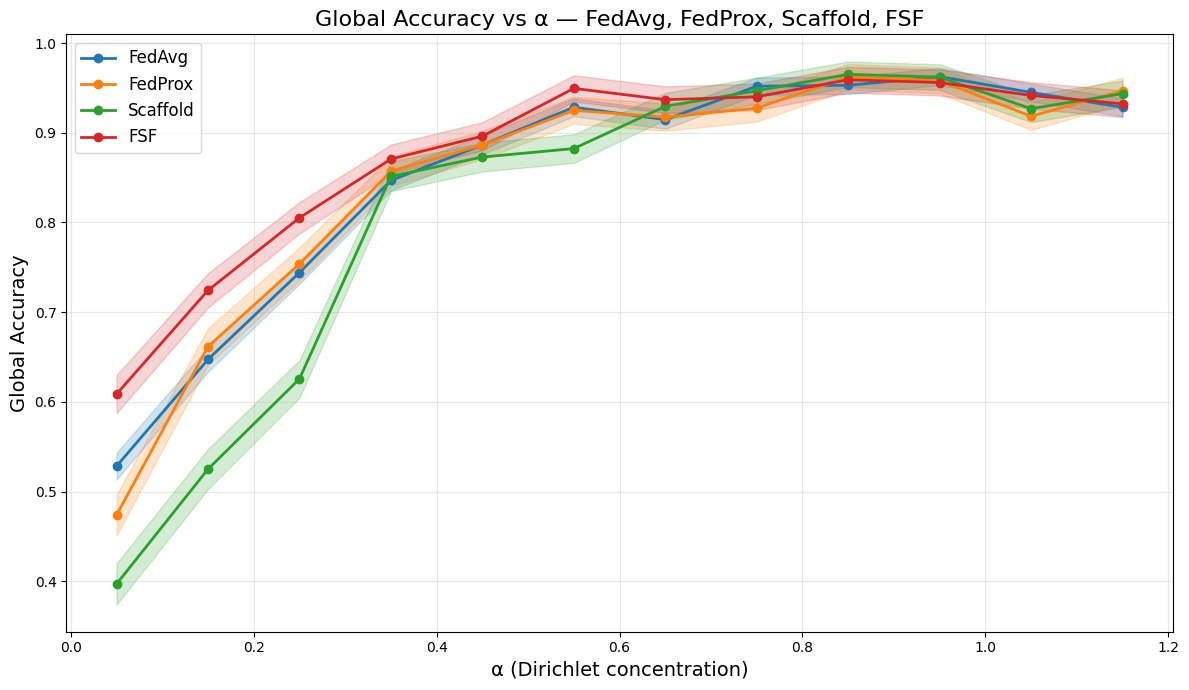
\includegraphics[width=217.587pt]{accuracy_FSF.jpg}};
    % Mask the existing opaque legend box, not the plotted data.
    \fill[white] (8,478) rectangle (136,589);
  \end{scope}
  \draw[black,line width=.25pt] (0,0) rectangle (1105,597);
  \foreach \x/\value in {4/0.0,187/0.2,370/0.4,553/0.6,735/0.8,918/1.0,1101/1.2}{
    \draw[black,line width=.25pt] (\x,0)--(\x,-9);
    \node[anchor=north] at (\x,-11) {\value};
  }
  \foreach \y/\value in {51/0.4,140/0.5,230/0.6,320/0.7,410/0.8,499/0.9,589/1.0}{
    \draw[black,line width=.25pt] (0,\y)--(-9,\y);
    \node[anchor=east] at (-11,\y) {\value};
  }
  \node at (552,636) {\textbf{(a)} Test accuracy};
  \node at (552,-95) {Dirichlet concentration $\alpha$};
\end{tikzpicture}
\hfill
\begin{tikzpicture}[x=.183pt,y=.183pt,every node/.style={font=\scriptsize,text=black}]
  \begin{scope}
    \clip (0,0) rectangle (1111,598);
    \node[anchor=south west,inner sep=0] at (-62,-58)
      {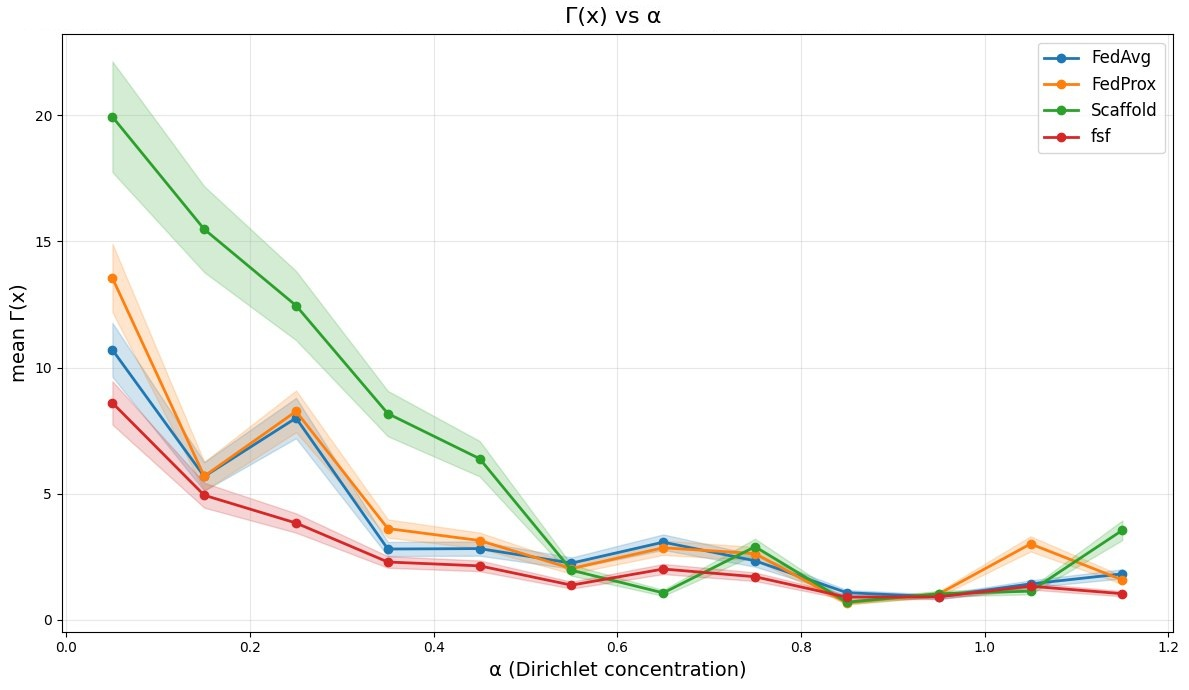
\includegraphics[width=217.587pt]{gamma_FSF.jpg}};
    % The covered region is the original opaque legend.
    \fill[white] (976,478) rectangle (1102,589);
  \end{scope}
  \draw[black,line width=.25pt] (0,0) rectangle (1111,598);
  \foreach \x/\value in {4/0.0,188/0.2,372/0.4,555/0.6,739/0.8,923/1.0,1106/1.2}{
    \draw[black,line width=.25pt] (\x,0)--(\x,-9);
    \node[anchor=north] at (\x,-11) {\value};
  }
  \foreach \y/\value in {12/0,138/5,264/10,391/15,517/20}{
    \draw[black,line width=.25pt] (0,\y)--(-9,\y);
    \node[anchor=east] at (-11,\y) {\value};
  }
  \node at (555,636) {\textbf{(b)} Classifier-gradient dispersion $\Gamma_t$};
  \node at (555,-95) {Dirichlet concentration $\alpha$};
\end{tikzpicture}
\caption{PathMNIST stress test: (a) test accuracy and (b) final-round
classifier-gradient dispersion $\Gamma_t$ from
Equation~\eqref{eq:gradient_dissimilarity}, versus Dirichlet concentration
$\alpha$. Dots indicate means across five independent runs; shaded areas
show the corresponding standard deviations.}
\label{fig:pathmnist_stress}
\end{figure*}

\begin{table*}[t]
\centering
\caption{\textbf{FEMNIST.} Writer-conditioned test performance and final-round classifier-gradient dissimilarity.}
\label{tab:femnist_results}
\begin{tabular}{lcccc}
\toprule
Method & Accuracy & $\Gamma_t$ & F1-Score & Balanced Accuracy \\
\midrule
FedAvg    & 85.49 $\pm 0.24$   & 0.83 $\pm 0.01$ & 66.87 $\pm 0.19$ & 67.09 $\pm 0.20$ \\
FedProx   & 84.73 $\pm 0.18$   & 0.81 $\pm 0.02$  & 64.16 $\pm 0.15$ & 65.81 $\pm 0.17$ \\
SCAFFOLD  & 84.51 $\pm 0.32$  & 0.78 $\pm 0.02$  & 65.68 $\pm 0.26$ & 66.46 $\pm 0.30$ \\
\textbf{FusedSpaceFed} & \textbf{86.82 $\pm 0.26$} & \textbf{0.71 $\pm 0.02$} & \textbf{68.77 $\pm 0.21$} & \textbf{68.38 $\pm 0.19$} \\
\bottomrule
\end{tabular}
\end{table*}
\subsection{Stress Test}
In addition to the five Dirichlet settings used in the main experiments, we
perform a separate stress-test sweep on PathMNIST using
$\alpha_j=0.05+0.10j$, $j=0,\ldots,11$.
This twelve-point grid corresponds to the values displayed in
Figure~\ref{fig:pathmnist_stress}.
This grid spans different levels of label heterogeneity, with lower $\alpha$
values yielding more concentrated client label distributions.

We train the four methods on PathMNIST for every
value in the stress-test grid and record test accuracy and classifier-gradient
dissimilarity after the final communication round. As shown in
Figure~\ref{fig:pathmnist_stress}(a), accuracy decreases for all methods
as the client partitions become more concentrated. FusedSpaceFed maintains the
highest accuracy in the strongest-skew portion of the sweep, while the
differences among methods narrow as $\alpha$ increases.
Figure~\ref{fig:pathmnist_stress}(b) shows the corresponding
classifier-gradient dispersion. FusedSpaceFed produces substantially lower
dispersion in the most heterogeneous settings and remains competitive over the
rest of the evaluated range.




\subsection{FEMNIST Benchmark}

We further evaluate all methods on \textbf{FEMNIST} from the \textsc{LEAF} benchmark~\cite{caldas2018leaf}, a widely adopted reference dataset for federated learning. FEMNIST consists of handwritten characters from thousands of distinct writers and exhibits natural client-level heterogeneity, as each client corresponds to a single user with highly skewed label and style distributions. This setting closely reflects realistic federated scenarios and is commonly used to assess robustness to client drift and non-IID data.

We retain LEAF's natural writer-level partition: each writer is one client,
with no pooling or repartitioning. Each round samples a subset of writers for
local training. Private FusedSpaceFed encoders and SCAFFOLD client control
variates persist when writers rejoin.

FedAvg, FedProx and SCAFFOLD use a shared classifier, whereas FusedSpaceFed
combines the shared decoder and classifier with writer-specific private
encoders. We therefore report writer-conditioned personalized test
performance: the test examples of each writer are processed using that
writer's private encoder together with the final shared decoder and classifier.

Gradient dissimilarity is evaluated after the final round using one
deterministic batch from each of 50 seeded writers and gradients with respect
to the classifier parameters only. Table~\ref{tab:femnist_results} reports the
mean results over five independent runs. FusedSpaceFed obtains the highest
writer-conditioned accuracy and the lowest measured final-round classifier
gradient dissimilarity among the evaluated methods.





%------------------------------------------
%------------------------------------------


\begin{coauthorrevision}
\paragraph{Contextual comparison with FedRep.}
Separately from the writer-level benchmark above, we evaluate FusedSpaceFed
on a reconstructed ten-letter setting inspired by
\citet{collins2021fedrep}: 150 synthetic clients, three classes per client,
and 10\% participation. With validation-selected learning rates, the
sample-weighted test accuracy is $79.05\pm2.68\%$ over five seeds, averaging
rounds 191--200 within each run (sample standard deviation across runs).
FedRep reports $78.56\%$ for its FEMNIST setting.
{\coauthordiffcolor Appendix~\ref{app:fedrep_comparison} details the experiment
and compares with published results for FedRep and other methods.}

\subsection{Feature Heterogeneity on Digits}
\label{sec:feature_heterogeneity_digits}

We further evaluate FusedSpaceFed on the five-domain Digits benchmark
considered by \citet{li2021fedbn}, comprising MNIST, SVHN, USPS,
SynthDigits, and MNIST-M. Each domain defines one client, providing a
common ten-class recognition task with heterogeneous image characteristics
across clients. Each client has 743 training examples, and all five clients
participate in each of 300 communication rounds. With hyperparameters
selected on a held-out validation split, FusedSpaceFed obtains a
final-round test accuracy of $85.86\pm0.85\%$, averaged uniformly across
domains and reported as mean $\pm$ sample standard deviation over five
independent runs. Appendix~\ref{app:feature_heterogeneity_digits} gives per-domain results,
published FedAvg, FedProx and FedBN reference values, and the protocol.

\paragraph{Component analysis.}
How do the individual components contribute to the predictive performance
of the complete fusion pipeline? We investigate reconstruction warm-up,
encoder sharing, and the original-input pathway on Digits using five paired
seeds and the same validation-selected hyperparameters. Retaining the
original input improves mean uniform-domain accuracy by 1.00 percentage
point relative to using the decoder output alone ($85.86\%$ versus
$84.86\%$). Removing warm-up yields $85.71\%$, while sharing the encoder
yields $86.18\%$. These comparisons support combining the original image
with the learned decoder output in this feature-heterogeneous setting,
with smaller mean changes under the other two interventions.
See Appendix~\ref{app:digits_ablation} for full results and protocol.

\subsection{Capacity and Computational Budget}
\label{sec:capacity_compute}

Using the same Digits setting and the five FusedSpaceFed runs reported
above, we additionally compare with a capacity- and compute-matched
FedAvg variant. The FedAvg classifier is widened to closely match the
number of active trainable parameters per client, and its local
optimization budget is adjusted to match the final training FLOPs of
FusedSpaceFed, including the reconstruction warm-up. Both methods use
the same data partition, preprocessing and evaluation protocol, with
hyperparameters selected separately on a common validation split.
Across five paired seeds, the final-round test accuracy, averaged
uniformly across the five domains, is $85.86\pm0.85\%$ for FusedSpaceFed
and $82.06\pm0.22\%$ for FedAvg (mean $\pm$ sample standard deviation
across runs). See Appendix~\ref{app:capacity_compute_comparison} for details.
\end{coauthorrevision}

\section{Conclusion}\label{sec:conclusion}

FusedSpaceFed combines private multiscale encoders with a shared decoder and
classifier through additive input fusion. Local training alternates
encoder-only reconstruction warm-up with end-to-end classification updates.
Our exact fixed-round decomposition identifies when fusion-induced variance
and cross-covariance reduce absolute classifier-gradient dispersion.
Experiments show higher average predictive performance than the reference
methods in most reported non-IID configurations and lower final-round
classifier-gradient dispersion on the evaluated subset of datasets.

\subsection{Current Limitations}

FusedSpaceFed requires persistent private encoders; unseen-client adaptation remains untested.

It adds computation, memory and decoder communication, with validation-selected $d_z$.

Evaluation is limited to image tasks with convolutional autoencoders and CNN or MLP classifiers; the analysis concerns individual rounds.

\subsection{Future Research Directions}

Encoder distillation, progressive encoder alignment or encoder-free inference
could enable a single deployable global model. Adaptive architectures could
reduce costs in larger federations and support sustainable
AI~\cite{amato2024sustainability,veglio2026scalerl}.

Further directions include heterogeneous or multimodal data, finite-sample
analyses of joint model evolution, hierarchical or clustered federations,
and evaluation under realistic communication and hardware constraints.
Representation-level mechanisms could also be combined with adaptive
optimization, including update rules selected using local gradients and
curvature~\cite{dicecco2027eva}. {\coauthordiffcolor A preliminary PathMNIST
experiment shows a substantial gain from federated refinement of the final
classifier on frozen representations (Appendix~\ref{app:pathmnist_head_refinement}).
Future work will assess robustness across seeds and datasets and the trade-off
between accuracy and additional communication.}

\clearpage
\section*{AI Use Statement}

In this work, we used generative AI tools to assist with manuscript editing, proofreading and revision; code cleanup, organization and debugging in preparation for the public repository; and bibliographic searches. We have reviewed all AI-assisted work. We take responsibility for the final content of this work, including text, claims, or artifacts produced with the aid of generative AI. 


%\backmatter

%\bmhead{Supplementary information}


%\bmhead{Acknowledgements}


%\section*{Declarations}


\bibliographystyle{apalike}
% Highlight the only bibliography entry added since the review baseline.
\begingroup
\let\coauthororiginalbibitem\bibitem
\def\coauthornewbibkey{luo2021nofear}
\renewcommand{\bibitem}[2][]{%
  \normalcolor%
  \coauthororiginalbibitem[#1]{#2}%
  \def\coauthorcurrentbibkey{#2}%
  \ifx\coauthorcurrentbibkey\coauthornewbibkey\coauthordiffcolor\fi%
}
\bibliography{references}% common bib file
\endgroup
%% if required, the content of .bbl file can be included here once bbl is generated
%%\input sn-article.bbl


%%%%%%%%%%%%%%%%%%%%%%%%%%%%%%%%%%%%%%%%%%%%%%%%%%%%%%%%%%%%
\section*{Checklist}
% Before submission, verify the affirmative answers against the actual
% anonymized experimental supplement, including natural writer-level FEMNIST
% training details and hardware. The coauthor/Overleaf ZIP is a manuscript
% source package and an internal evidence archive, not that supplement.


% %%% BEGIN INSTRUCTIONS %%%
%The checklist follows the references. For each question, choose your answer from the three possible options: Yes, No, Not Applicable.  You are encouraged to include a justification to your answer, either by referencing the appropriate section of your paper or providing a brief inline description (1-2 sentences).
%Please do not modify the questions.  Note that the Checklist section does not count towards the page limit. Not including the checklist in the first submission won't result in desk rejection, although in such case we will ask you to upload it during the author response period and include it in camera ready (if accepted).

%\textbf{In your paper, please delete this instructions block and only keep the Checklist section heading above along with the questions/answers below.}
% %%% END INSTRUCTIONS %%%


\begin{enumerate}

  \item For all models and algorithms presented, check if you include:
  \begin{enumerate}
    \item A clear description of the mathematical setting, assumptions, algorithm, and/or model. [Yes]
    \item An analysis of the properties and complexity (time, space, sample size) of any algorithm. [Yes]
    \item (Optional) Anonymized source code, with specification of all dependencies, including external libraries. [Yes]
  \end{enumerate}

  \item For any theoretical claim, check if you include:
  \begin{enumerate}
    \item Statements of the full set of assumptions of all theoretical results. [Yes]
    \item Complete proofs of all theoretical results. [Yes]
    \item Clear explanations of any assumptions. [Yes]
  \end{enumerate}

  \item For all figures and tables that present empirical results, check if you include:
  \begin{enumerate}
    \item The code, data, and instructions needed to reproduce the main experimental results (either in the supplemental material or as a URL). [Yes]
    \item All the training details (e.g., data splits, hyperparameters, how they were chosen). [Yes]
    \item A clear definition of the specific measure or statistics and error bars (e.g., with respect to the random seed after running experiments multiple times). [Yes]
    \item A description of the computing infrastructure used. (e.g., type of GPUs, internal cluster, or cloud provider). [Yes]
  \end{enumerate}

  \item If you are using existing assets (e.g., code, data, models) or curating/releasing new assets, check if you include:
  \begin{enumerate}
    \item Citations of the creator If your work uses existing assets. [Yes]
    \item The license information of the assets, if applicable. [Not Applicable]
    \item New assets either in the supplemental material or as a URL, if applicable. [Not Applicable]
    \item Information about consent from data providers/curators. [Not Applicable]
    \item Discussion of sensible content if applicable, e.g., personally identifiable information or offensive content. [Not Applicable]
  \end{enumerate}

  \item If you used crowdsourcing or conducted research with human subjects, check if you include:
  \begin{enumerate}
    \item The full text of instructions given to participants and screenshots. [Not Applicable]
    \item Descriptions of potential participant risks, with links to Institutional Review Board (IRB) approvals if applicable. [Not Applicable]
    \item The estimated hourly wage paid to participants and the total amount spent on participant compensation. [Not Applicable]
  \end{enumerate}

\end{enumerate}


\clearpage
\appendix
\begin{coauthorrevision}
\section{\texorpdfstring{\coauthordiffcolor Reconstructed FEMNIST Comparison with Published Baselines}{Reconstructed FEMNIST Comparison with Published Baselines}}
\label{app:fedrep_comparison}

\subsection{Scope and data reconstruction}

This experiment places FusedSpaceFed alongside the published FEMNIST
results of \citet{collins2021fedrep}. We construct 150 synthetic clients
from the ten lowercase letters a--j, with three classes per client.

We use the NIST Special Database 19 \texttt{by\_class.zip} archive,
specifically the \texttt{train\_}\textit{class} PNG directories.
Images are converted to grayscale $28\times28$ inputs in $[0,1]$, preserving
orientation, with no augmentation. Following the historical generator's
recipe, each class pool contains at most 4,000 images. Client $i$, indexed
from zero, receives classes $(i+j)\bmod10$, $j=0,1,2$, with requested
per-class count $\lfloor(\exp Z_i+100)/3\rfloor$, where
$Z_i\sim\mathcal{N}(4,1)$; the data seed is 20261003.

The requested totals exceed the available pools for f (2,555 requested,
2,493 available), i (3,078; 2,788), and j (3,196; 1,920). For these classes
only, we reduce each client's quota proportionally and allocate integer
remainders in decreasing fractional-remainder order, breaking ties by
client ID. This changes the quotas of 105 clients. All assigned classes
are retained, and each source image is assigned at most once globally.
Each client is shuffled and split into $\lfloor0.9N_i\rfloor$ training
examples and the remaining test examples, using split seed 20261004.
The resulting fixed partition contains 25,339 images: 22,736 training and
2,603 test, with disjoint source identifiers across clients and splits.
All five runs use this same partition; variability across partitions is
not measured.

\subsection{Model and training choices}

The classifier is an MLP with widths $784,512,256,64,10$, biases, and ReLU
after each hidden layer. The classifier dimensions follow the FedRep
source code. We apply cross-entropy to logits.

FusedSpaceFed retains its private persistent encoder and shared decoder,
using the compact U-Net with base width 16 and $d_z=64$. The decoder has
a linear output, and fusion is $x+D(E_i(x))$, without clamping or extra
normalization. Each of 200 rounds samples 15 clients uniformly without
replacement. With batch size 10, a selected client performs one epoch
of encoder-only MSE warm-up, followed by five epochs of cross-entropy
training of encoder, decoder, and classifier. The latter phase has no
reconstruction loss. Decoder and classifier updates are averaged
uniformly across selected clients.

The selected classifier optimizer is SGD with learning rate 0.02,
momentum 0.5, weight decay $10^{-4}$ on weights and zero on biases.
Encoder and decoder use Adam with learning rate $3\times10^{-4}$,
$\beta=(0.9,0.999)$, $\epsilon=10^{-8}$, and no weight decay.
Active gradients are clipped to L2 norm 1.0 separately for each optimizer.
Optimizers restart at each client participation; Adam state persists
between the two local phases. Learning rates are constant. Computation
uses Float32 with AMP and TF32 disabled.

\subsection{Validation-based calibration}

Calibration uses only the original training portion. Within each
client--class group, $\lfloor n/5\rfloor$ examples are held out using a
deterministic hash ordering with seed 20261004, leaving 18,374 fit and
4,362 validation examples. Six configurations are specified in advance,
as triples (classifier learning rate, autoencoder learning rate, clipping
norm): $(0.01,0.001,1)$, $(0.01,0.0003,1)$, $(0.01,0.0001,1)$,
$(0.02,0.0003,1)$, $(0.005,0.0003,1)$, and $(0.01,0.0003,2)$.

All six are screened for 80 rounds with seed 141, using sample-weighted
validation accuracy averaged over rounds 71--80. The reference and the
two highest-scoring alternatives are extended to 200 rounds and also
run with seed 142. Selection uses the mean of the two seeds' validation
accuracies over rounds 191--200. The chosen triple $(0.02,0.0003,1)$
obtains $88.77\%$ on this selection criterion. It is frozen before the
five final runs, which start afresh with seeds 41--45 and use all 22,736
original training examples.

\subsection{Evaluation and results}

After each of rounds 191--200, all 150 clients are evaluated on their
original local test examples, using the current shared decoder and
classifier and their persistent private encoder, without test-time
adaptation. For seed $s$ and round $t$, let $c_{s,t,i}$ be the number of
correct predictions on client $i$ and $n_i$ its test-set size. Our primary
and secondary accuracies are, respectively,
\[
 A_{s,t}=100\frac{\sum_i c_{s,t,i}}{\sum_i n_i},
 \qquad
 U_{s,t}=\frac{100}{150}\sum_i\frac{c_{s,t,i}}{n_i}.
\]
We average ten rounds within each seed, then report the mean and sample
standard deviation ($n-1$ denominator) across five seed means.
All runs complete 200 rounds; no best seed, round, or checkpoint is selected.

The primary result is $79.05\pm2.68\%$; the uniform-client result is
$80.90\pm2.81\%$ (Table~\ref{tab:fedrep_reconstructed_seeds}).
Table~\ref{tab:fedrep_published_comparison} presents the comparison with
the published FEMNIST reference values.

\begin{table*}[t]
\coauthorcolor
\begin{minipage}[t]{0.48\textwidth}
\centering
\caption{Accuracy (\%) by seed on our fixed reconstructed partition.
Each entry averages rounds 191--200. SD is across five seed means.}
\label{tab:fedrep_reconstructed_seeds}
\begin{tabular}{lrr}
\toprule
Seed & Sample-weighted & Uniform-client \\
\midrule
41 & 82.34 & 84.39 \\
42 & 75.26 & 77.77 \\
43 & 77.71 & 78.31 \\
44 & 80.21 & 82.47 \\
45 & 79.72 & 81.57 \\
\midrule
Mean & 79.05 & 80.90 \\
Sample SD & 2.68 & 2.81 \\
\bottomrule
\end{tabular}
\end{minipage}\hfill
\begin{minipage}[t]{0.48\textwidth}
\centering
\caption{Published FEMNIST reference values from Table~1 of
\citet{collins2021fedrep}, column $(150,3)$, and our separately measured
result. Bold indicates the highest reported mean accuracy.}
\label{tab:fedrep_published_comparison}
\begin{tabular}{lr}
\toprule
Method & Accuracy (\%) \\
\midrule
\multicolumn{2}{l}{\textit{Published; uncertainty not reported}} \\
Local Only & 60.86 \\
FedAvg & 51.64 \\
FedAvg+FT & 72.41 \\
FedProx & 18.89 \\
FedProx+FT & 53.54 \\
SCAFFOLD & 17.65 \\
SCAFFOLD+FT & 52.11 \\
Fed-MTL & 54.11 \\
PerFedAvg & 71.51 \\
LG-Fed & 62.08 \\
L2GD & 66.18 \\
APFL & 70.74 \\
Ditto & 68.28 \\
FedPer & 76.91 \\
FedRep & 78.56 \\
\midrule
\multicolumn{2}{l}{\textit{Ours; reconstructed partition, mean $\pm$ SD}} \\
FusedSpaceFed, calibrated & $\boldsymbol{79.05\pm2.68}$ \\
\bottomrule
\end{tabular}
\end{minipage}
\end{table*}

\section{Capacity- and Compute-Matched Comparison with FedAvg}
\label{app:capacity_compute_comparison}

\subsection{Digits setting and model}

We use the five-domain Digits benchmark associated with
\citet{li2021fedbn}: MNIST, SVHN, USPS, SynthDigits and MNIST-M.
Each domain is assigned to one client with 743 training images, giving
3,715 training images in total. The fixed training partition and the full
domain test sets are used for both methods. Images are represented as
three-channel $28\times28$ inputs, with pixel values normalized to
$[-1,1]$. All five clients participate in each of 300 communication rounds,
and shared states are aggregated uniformly.

The classifier has three convolutional layers with channel widths
$3,64,64,128$, followed by fully connected layers with widths
$6272,2048,512,10$. Its batch-normalization parameters and buffers are shared.
FusedSpaceFed uses a compact U-Net with base width 16 and bottleneck
width $d_z=64$, a persistent private encoder for each client, and a shared
decoder. Classification uses the fused input $x+D(E_i(x))$.

For FedAvg, the first fully connected layer is widened from 2048 to 2065
units; the following layer and the corresponding batch-normalization
layer are adjusted accordingly. The active parameter count per client is
14,336,285 for FusedSpaceFed, comprising 14,219,210 classifier parameters,
72,080 encoder parameters and 44,995 decoder parameters.
The enlarged FedAvg classifier has 14,334,589 parameters, a relative
difference of $0.01183\%$. FusedSpaceFed stores its five client encoders
separately, together with the shared decoder and classifier.

\subsection{Local optimization and FLOP budget}

Each FusedSpaceFed client performs one encoder-only reconstruction epoch
with the decoder frozen, followed by one classification epoch updating
the encoder, decoder and classifier. Reconstruction uses mean squared
error; classification uses cross-entropy. The maximum batch size is 32,
and the final batch of each epoch is retained.

The FedAvg local workload is set using the combined reconstruction and
classification FLOP budget of FusedSpaceFed for each client and round.
It comprises one pass through the local training set followed by additional
shuffled minibatches. Batch sizes are selected using integer arithmetic,
and the unspent remainder is carried to subsequent rounds.

Dense forward and backward operations are counted with Torch 2.5.1
\texttt{FlopCounterMode}, assigning two FLOPs to a fused multiply-add.
The count includes gradient propagation through the frozen decoder during
reconstruction. Optimizer updates and gradient-norm clipping are accounted
for using $5P$ scalar operations per SGD step and $16P$ per Adam step,
where $P$ is the number of parameters updated by that optimizer.
Batch normalization, activations, pooling, loss evaluation, finite-value
checks, copies, aggregation and kernel overhead are outside this FLOP
accounting convention.

Table~\ref{tab:capacity_compute_resources} gives the cumulative counts
per final run. The relative difference in counted training FLOPs is
$0.000198\%$. Across all clients and rounds, FusedSpaceFed performs
36,000 reconstruction steps and 36,000 classification steps; FedAvg
performs 63,000 classification steps. The corresponding numbers of
supervised sample presentations are 1,114,500 and 1,956,535.

\begin{table}[H]
\coauthorcolor
\centering
\small
\setlength{\tabcolsep}{4pt}
\caption{Active parameters per client and cumulative training FLOPs
per run. The FusedSpaceFed FLOP count includes reconstruction warm-up.}
\label{tab:capacity_compute_resources}
\begin{tabular}{lrr}
\toprule
Method & Parameters & FLOPs ($10^{12}$) \\
\midrule
FusedSpaceFed & 14,336,285 & 551.898005 \\
FedAvg, enlarged & 14,334,589 & 551.896914 \\
\bottomrule
\end{tabular}
\end{table}

\subsection{Validation-based calibration}

For each domain, 149 of the 743 training images are assigned to
validation and 594 to fitting, using deterministic class-stratified
selection with data seed 20261005. The same split is used by both
methods.

For FedAvg, nine configurations are evaluated for 60 rounds with
seed 142, combining classifier learning rates
$\{0.005,0.01,0.02\}$ and gradient-clipping norms $\{0.5,1,2\}$.
Selection uses the uniform mean of domain validation accuracies at
round 60 and yields classifier learning rate 0.02 and clipping norm 2.

FusedSpaceFed uses the validation-selected configuration described in
Appendix~\ref{app:feature_heterogeneity_digits}. Candidate configurations
are screened for 120 rounds and shortlisted configurations are confirmed
over 300 rounds using two validation seeds. The selected configuration
uses classifier learning rate 0.1, autoencoder learning rate
$3\times10^{-4}$, and clipping norm 10.

The classifier optimizer is SGD with zero momentum and weight decay.
Encoder and decoder use Adam with $\beta=(0.9,0.999)$,
$\epsilon=10^{-8}$ and zero weight decay. Optimizers are initialized at
each client participation, with Adam state retained between the two
local phases. Learning rates are constant. Computation uses Float32
with AMP and TF32 disabled.

The selected configurations are fixed before the final runs.
Both methods are trained from scratch on all 743 training images per
client for 300 rounds, using paired seeds 42--46.

\subsection{Evaluation and results}

At round 300, each client is evaluated on its domain's full test set.
FusedSpaceFed predictions combine that client's encoder with the final
shared decoder and classifier; FedAvg uses its final shared classifier.
Evaluation uses inference mode and the parameters obtained from training.

Let $c_{s,d}$ and $n_d$ denote the correct-prediction count and test-set
size for seed $s$ and domain $d$, respectively. The uniform-domain
primary accuracy and the sample-weighted accuracy are, respectively,
\[
 U_s=\frac{100}{5}\sum_{d=1}^{5}\frac{c_{s,d}}{n_d},
 \qquad
 A_s=100\frac{\sum_{d=1}^{5}c_{s,d}}{\sum_{d=1}^{5}n_d}.
\]
We report means and sample standard deviations across the five paired
seeds, using the $n-1$ denominator. The uniform-domain accuracy is
$85.86\pm0.85\%$ for FusedSpaceFed and $82.06\pm0.22\%$ for FedAvg.
Table~\ref{tab:capacity_compute_seeds} reports the primary result and
paired differences. The sample-weighted result is $84.51\pm0.75\%$
for FusedSpaceFed and $79.68\pm0.39\%$ for FedAvg.
Table~\ref{tab:capacity_compute_domains} gives the domain-level results.

\begin{table}[H]
\coauthorcolor
\centering
\small
\setlength{\tabcolsep}{4pt}
\caption{Final-round uniform-domain accuracy (\%) and paired difference
(FusedSpaceFed minus FedAvg, in percentage points).
Bold indicates the higher accuracy in each row.}
\label{tab:capacity_compute_seeds}
\begin{tabular}{lrrr}
\toprule
Seed & FusedSpaceFed & FedAvg & Difference \\
\midrule
42 & \textbf{84.67} & 82.27 & $+2.40$ \\
43 & \textbf{86.30} & 82.15 & $+4.15$ \\
44 & \textbf{85.32} & 82.25 & $+3.08$ \\
45 & \textbf{86.76} & 81.78 & $+4.98$ \\
46 & \textbf{86.26} & 81.89 & $+4.37$ \\
\midrule
Mean & \textbf{85.86} & 82.06 & $+3.80$ \\
Sample SD & 0.85 & 0.22 & 1.04 \\
\bottomrule
\end{tabular}
\end{table}

\begin{table}[H]
\coauthorcolor
\centering
\small
\setlength{\tabcolsep}{4pt}
\caption{Final-round domain accuracy (\%): mean and sample standard
deviation across five seeds.
Bold indicates the higher mean accuracy in each row.}
\label{tab:capacity_compute_domains}
\begin{tabular}{lrr}
\toprule
Domain & FusedSpaceFed & FedAvg \\
\midrule
MNIST & $\boldsymbol{96.95\pm0.24}$ & $95.93\pm0.24$ \\
SVHN & $\boldsymbol{67.83\pm2.88}$ & $61.57\pm1.43$ \\
USPS & $\boldsymbol{96.67\pm0.28}$ & $95.94\pm0.25$ \\
SynthDigits & $\boldsymbol{86.32\pm0.50}$ & $81.31\pm0.54$ \\
MNIST-M & $\boldsymbol{81.55\pm0.77}$ & $75.58\pm0.64$ \\
\bottomrule
\end{tabular}
\end{table}

\begin{table*}[t]
\coauthorcolor
\centering
\small
\setlength{\tabcolsep}{9pt}
\caption{Test accuracy (\%) on the five-domain Digits benchmark.
Published reference values for FedAvg, FedProx, and FedBN are taken from
Table~11 of the supplementary material of \citet{li2021fedbn}.
FusedSpaceFed results are mean $\pm$ sample standard deviation over five
independent runs, evaluated at communication round 300.
Bold indicates the highest reported mean accuracy in each row.}
\label{tab:feature_heterogeneity_digits}
\begin{tabular}{lrrrr}
\toprule
Domain & \shortstack{FedAvg\\published} & \shortstack{FedProx\\published}
       & \shortstack{FedBN\\published} & \shortstack{FusedSpaceFed\\ours} \\
\midrule
MNIST       & $97.38\pm0.05$ & $97.30\pm0.17$ & $\boldsymbol{97.55\pm0.11}$ & $96.95\pm0.24$ \\
SVHN        & $70.59\pm0.51$ & $71.55\pm0.75$ & $\boldsymbol{76.93\pm0.25}$ & $67.83\pm2.88$ \\
USPS        & $96.91\pm0.11$ & $96.98\pm0.19$ & $\boldsymbol{97.69\pm0.10}$ & $96.67\pm0.28$ \\
SynthDigits & $86.66\pm0.21$ & $86.60\pm0.18$ & $\boldsymbol{87.46\pm0.20}$ & $86.32\pm0.50$ \\
MNIST-M     & $82.44\pm0.41$ & $82.67\pm0.75$ & $\boldsymbol{83.57\pm0.38}$ & $81.55\pm0.77$ \\
\bottomrule
\end{tabular}
\end{table*}

\newpage
\section{Feature Heterogeneity on Digits}
\label{app:feature_heterogeneity_digits}

We use the data partition, preprocessing, and FusedSpaceFed architecture
described in Appendix~\ref{app:capacity_compute_comparison}. Each domain
contributes 743 training examples, with the class frequencies present in
the distributed partition. Images are represented as three-channel
$28\times28$ inputs normalized to $[-1,1]$. All five clients participate
in every round, with uniform aggregation of the shared decoder and
classifier. The classifier's batch-normalization parameters and running
statistics are included in its shared state.

Hyperparameter selection uses a fixed split of 594 training and 149
validation examples per client. Candidate configurations are screened for
120 rounds, followed by 300-round confirmation of shortlisted
configurations using two validation seeds. Selection is based on the mean
final-round validation accuracy across domains and confirmation seeds.
The selected configuration uses classifier SGD with learning rate 0.1,
encoder--decoder Adam with learning rate 0.0003, and gradient-norm clipping
at 10. Each communication round includes one encoder-only reconstruction
warm-up epoch followed by one end-to-end classification epoch, with batch
size 32.

The selected configuration is then trained from scratch on all 743
training examples per client using seeds 42--46. At round 300, each
client-conditioned predictor is evaluated on its domain's test set.
We report the mean and sample standard deviation across the five runs
for each domain in Table~\ref{tab:feature_heterogeneity_digits}.
The uniform mean across domains is computed within each run and then
summarized across runs.

Unlike our severe label-skew experiments, the Digits benchmark primarily
evaluates feature heterogeneity, which FedBN is specifically designed to
address. This difference in regime may partly explain the gap to the
published FedBN results, although validating this hypothesis would
require further controlled experiments.

% Results archived at d13c1a0c3131ba81adbeb911a50aa3f92d5aafe9.
% Numeric tables are generated from the unmodified JSON files in
% ../evidence/digits/ by ../scripts/build_digits_tables.py.
\clearpage
\section{Component and Gradient Diagnostics on Digits}
\label{app:digits_diagnostics}

We use the five calibrated FusedSpaceFed runs (seeds 42--46) reported in
Sections~\ref{sec:feature_heterogeneity_digits} and \ref{sec:capacity_compute}.
The data partition, architecture, and validation-selected hyperparameters
are those in Appendices~\ref{app:capacity_compute_comparison} and
\ref{app:feature_heterogeneity_digits}. The full-model reference is therefore
the same $85.86\pm0.85\%$ uniform-domain accuracy reported in the main text.

\subsection{Decoder Behavior and Reconstruction Warm-Up}
\label{app:digits_decoder}

What role does reconstruction warm-up play before task-driven optimization?
We replay one local participation from copies of the initial and final
(round 300) checkpoints of the five full-model runs, using a fixed training
probe of 160 examples per domain, arranged in five batches of 32.
Each replay performs one encoder-only warm-up epoch followed by one
end-to-end classification epoch. Optimizers are reset at the start of
participation, as in the Digits training protocol, with continuous Adam
state between the two phases. Metrics are evaluated with frozen BatchNorm
statistics. The intermediate states are local diagnostic replays from the
saved checkpoints.

Warm-up reduces reconstruction MSE averaged across seeds in every domain
at both checkpoint stages (Table~\ref{tab:digits_reconstruction}).
At the final checkpoints, MSE averaged across domains and seeds decreases
from 0.4512 to 0.4477 after warm-up, then increases to 0.5028 after
classification. These observations illustrate the distinct roles of the
two phases: warm-up improves reconstruction, whereas subsequent
classification shapes the decoder output through the prediction objective
alone.

\begin{table*}[t]
\coauthorcolor
\centering
\small
\setlength{\tabcolsep}{8pt}
\caption{Reconstruction MSE on the fixed Digits training probes, averaged over five seeds. Each checkpoint is copied before a local replay. Before, Warm-up, and Classification denote successive replay states; the two column groups start from initialization and round 300.}
\label{tab:digits_reconstruction}
\begin{tabular}{lrrrrrr}
\toprule
& \multicolumn{3}{c}{Initial checkpoints} & \multicolumn{3}{c}{Final checkpoints} \\
\cmidrule(lr){2-4}\cmidrule(lr){5-7}
Domain & Before & Warm-up & Classification & Before & Warm-up & Classification \\
\midrule
MNIST & 0.9428 & 0.9213 & 0.9239 & 0.9023 & 0.8962 & 1.1163 \\
SVHN & 0.1965 & 0.1921 & 0.1924 & 0.1877 & 0.1853 & 0.1955 \\
USPS & 0.5946 & 0.5804 & 0.5813 & 0.5649 & 0.5611 & 0.5715 \\
SynthDigits & 0.3730 & 0.3656 & 0.3670 & 0.3517 & 0.3482 & 0.3668 \\
MNIST-M & 0.2845 & 0.2795 & 0.2772 & 0.2496 & 0.2475 & 0.2639 \\
\bottomrule
\end{tabular}
\end{table*}


The decoder ends with a linear convolution, allowing output values beyond
the normalized input range $[-1,1]$. Figure~\ref{fig:digits_decoder_probe}
illustrates the image-space signals before and after each phase.
All measured outputs, losses, and model states remain finite in these
replays. During warm-up, only the encoder changes; classification updates
the encoder, decoder, and classifier.

\begin{figure*}[t]
\coauthorcolor
\centering
\setlength{\tabcolsep}{5pt}
\begin{tabular}{rccccc}
 & MNIST & SVHN & USPS & SynthDigits & MNIST-M \\
\raisebox{.20in}{\scriptsize\shortstack[r]{Input}} & 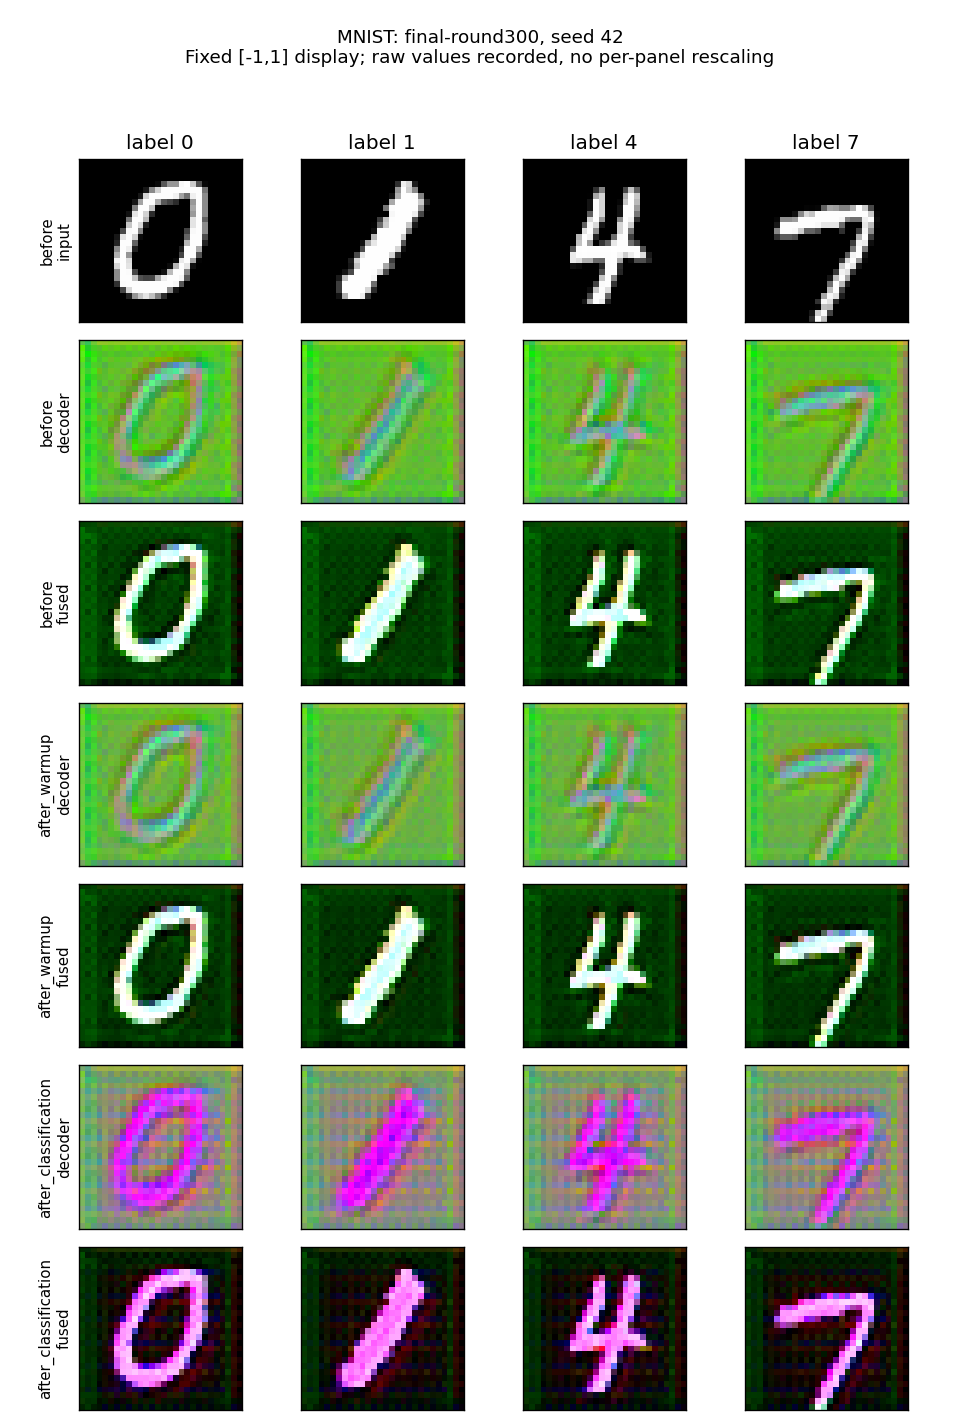
\includegraphics[width=.56in,trim=47.4bp 663.0bp 430.2bp 95.4bp,clip]{figures/digits/final-round300-MNIST.png} & 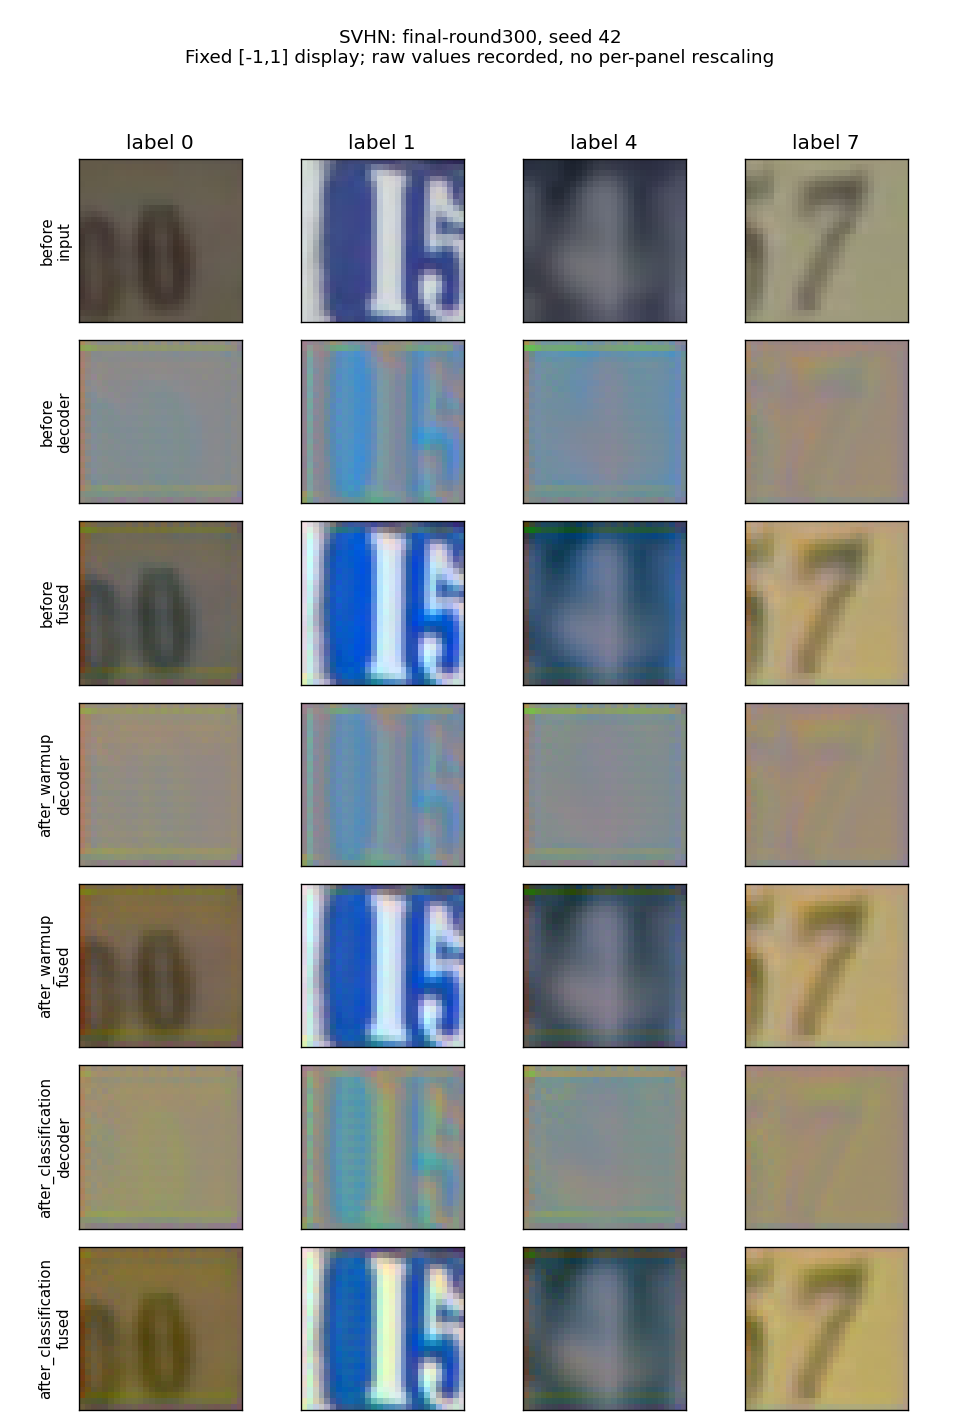
\includegraphics[width=.56in,trim=47.4bp 663.0bp 430.2bp 95.4bp,clip]{figures/digits/final-round300-SVHN.png} & 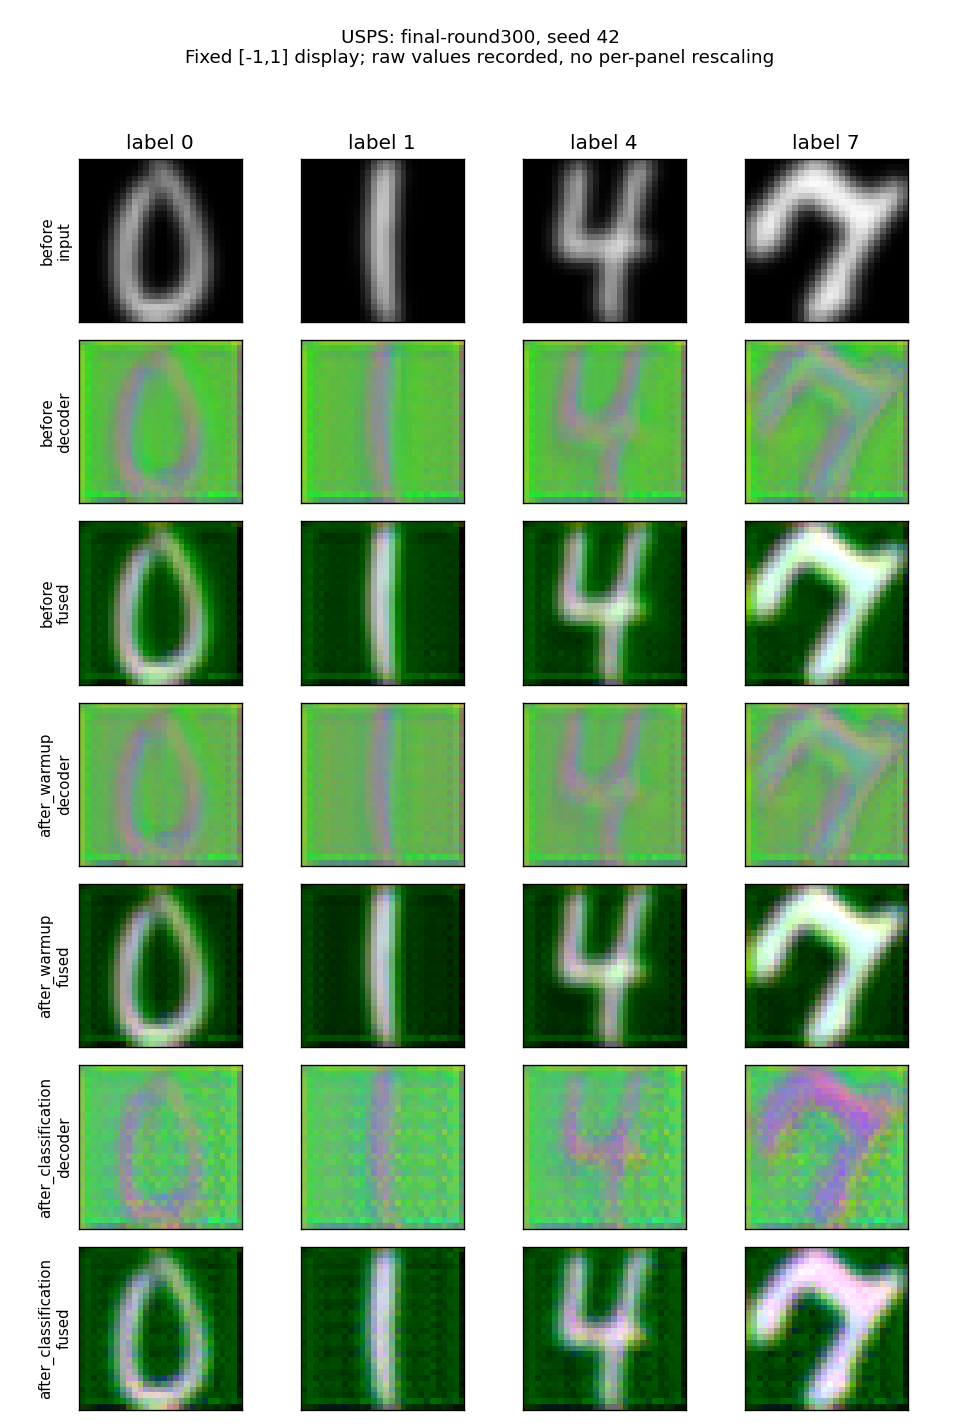
\includegraphics[width=.56in,trim=47.4bp 663.0bp 430.2bp 95.4bp,clip]{figures/digits/final-round300-USPS.png} & 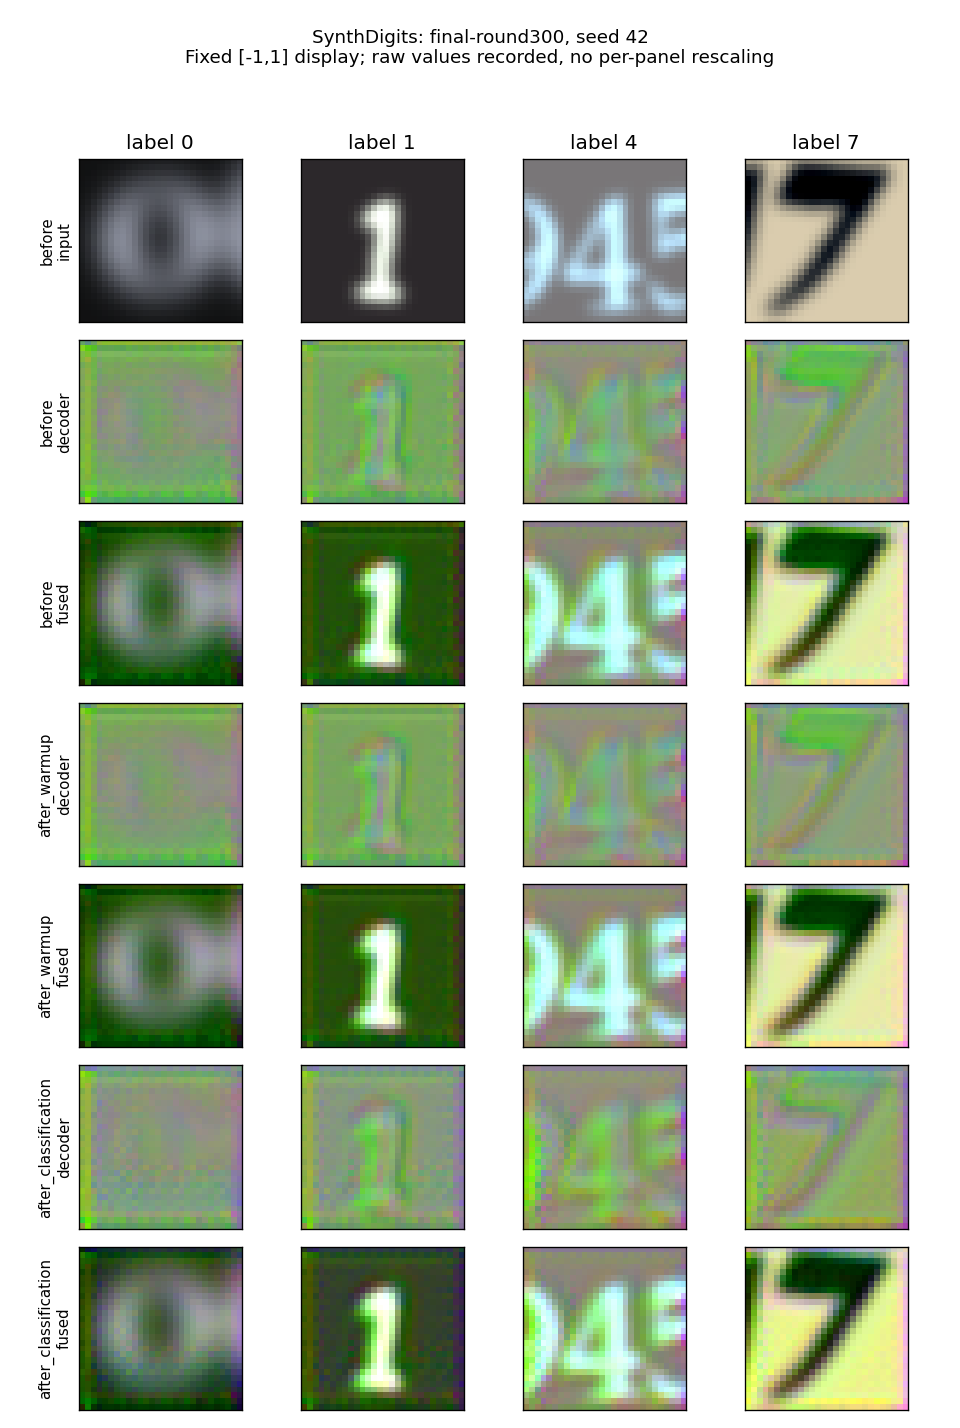
\includegraphics[width=.56in,trim=47.4bp 663.0bp 430.2bp 95.4bp,clip]{figures/digits/final-round300-SynthDigits.png} & 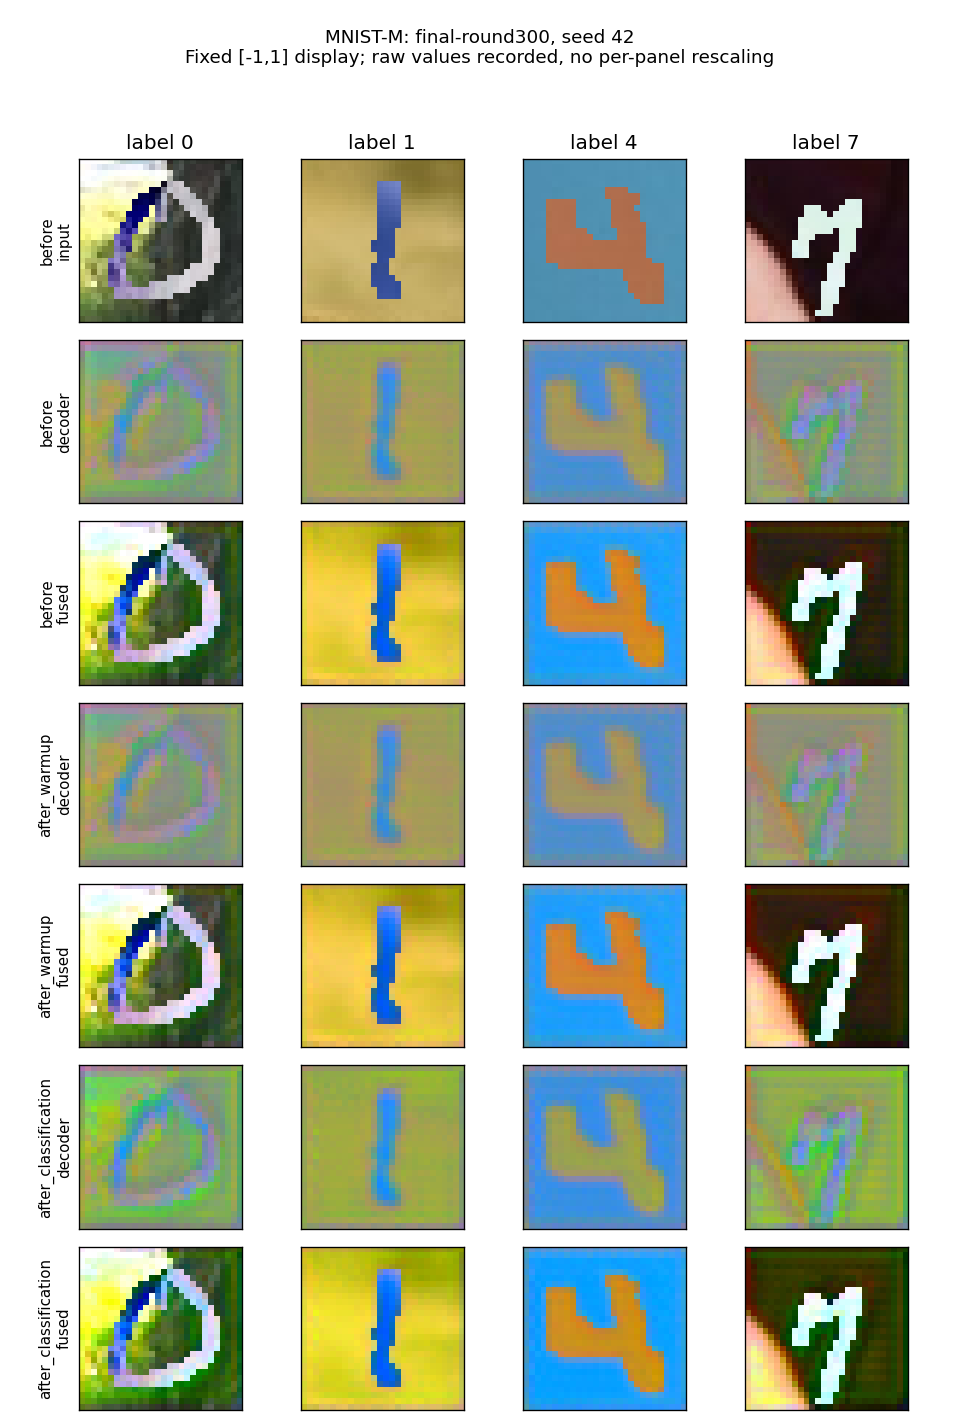
\includegraphics[width=.56in,trim=47.4bp 663.0bp 430.2bp 95.4bp,clip]{figures/digits/final-round300-MNIST-M.png} \\[-2pt]
\raisebox{.20in}{\scriptsize\shortstack[r]{Before\\decoder}} & 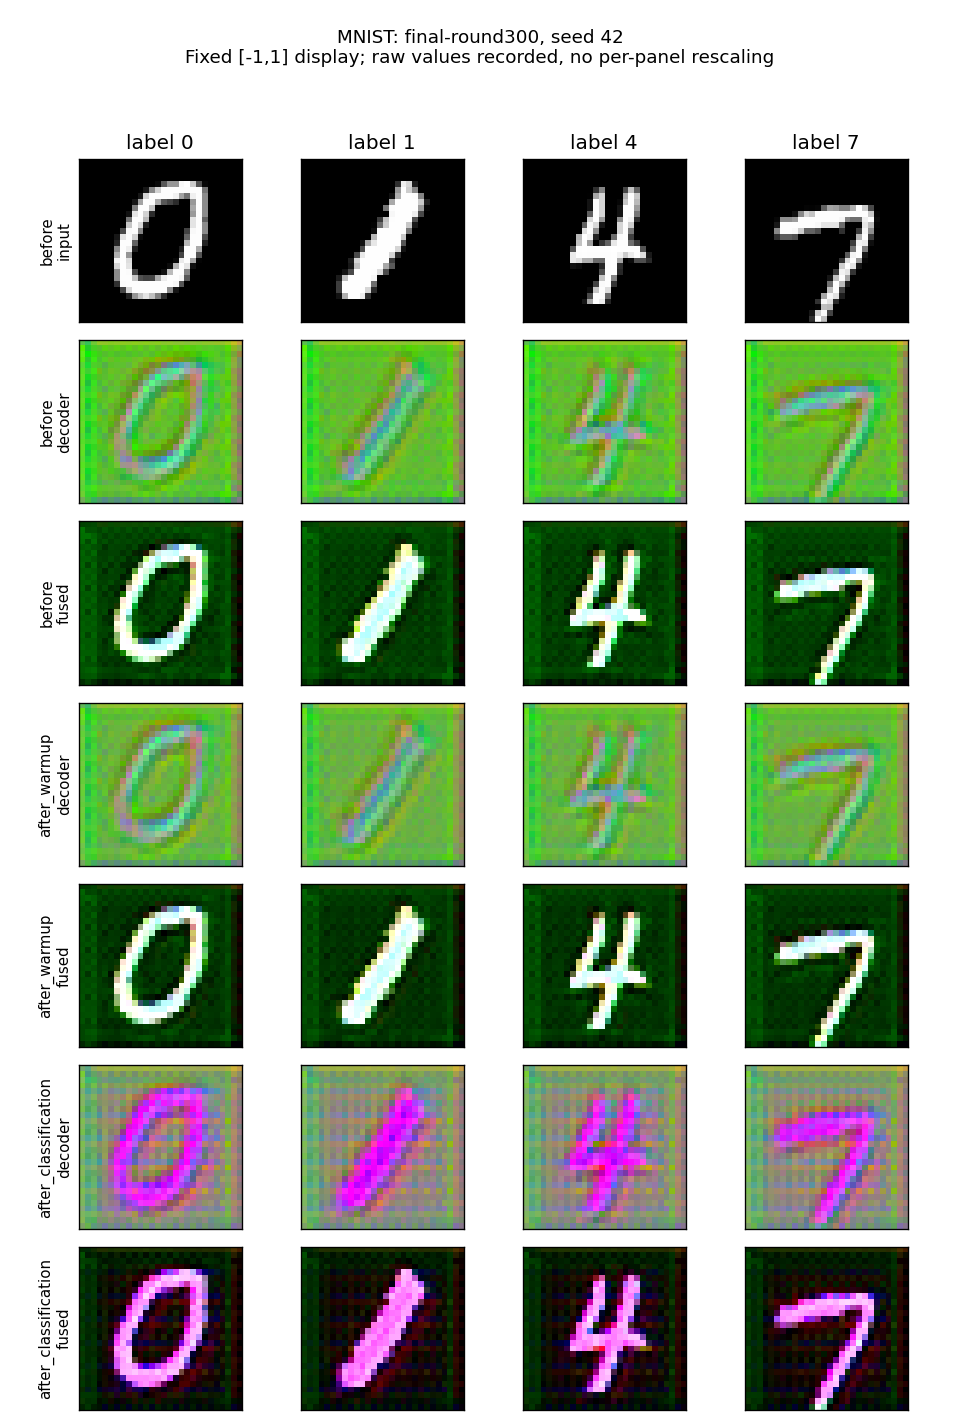
\includegraphics[width=.56in,trim=47.4bp 554.4bp 430.2bp 204.0bp,clip]{figures/digits/final-round300-MNIST.png} & 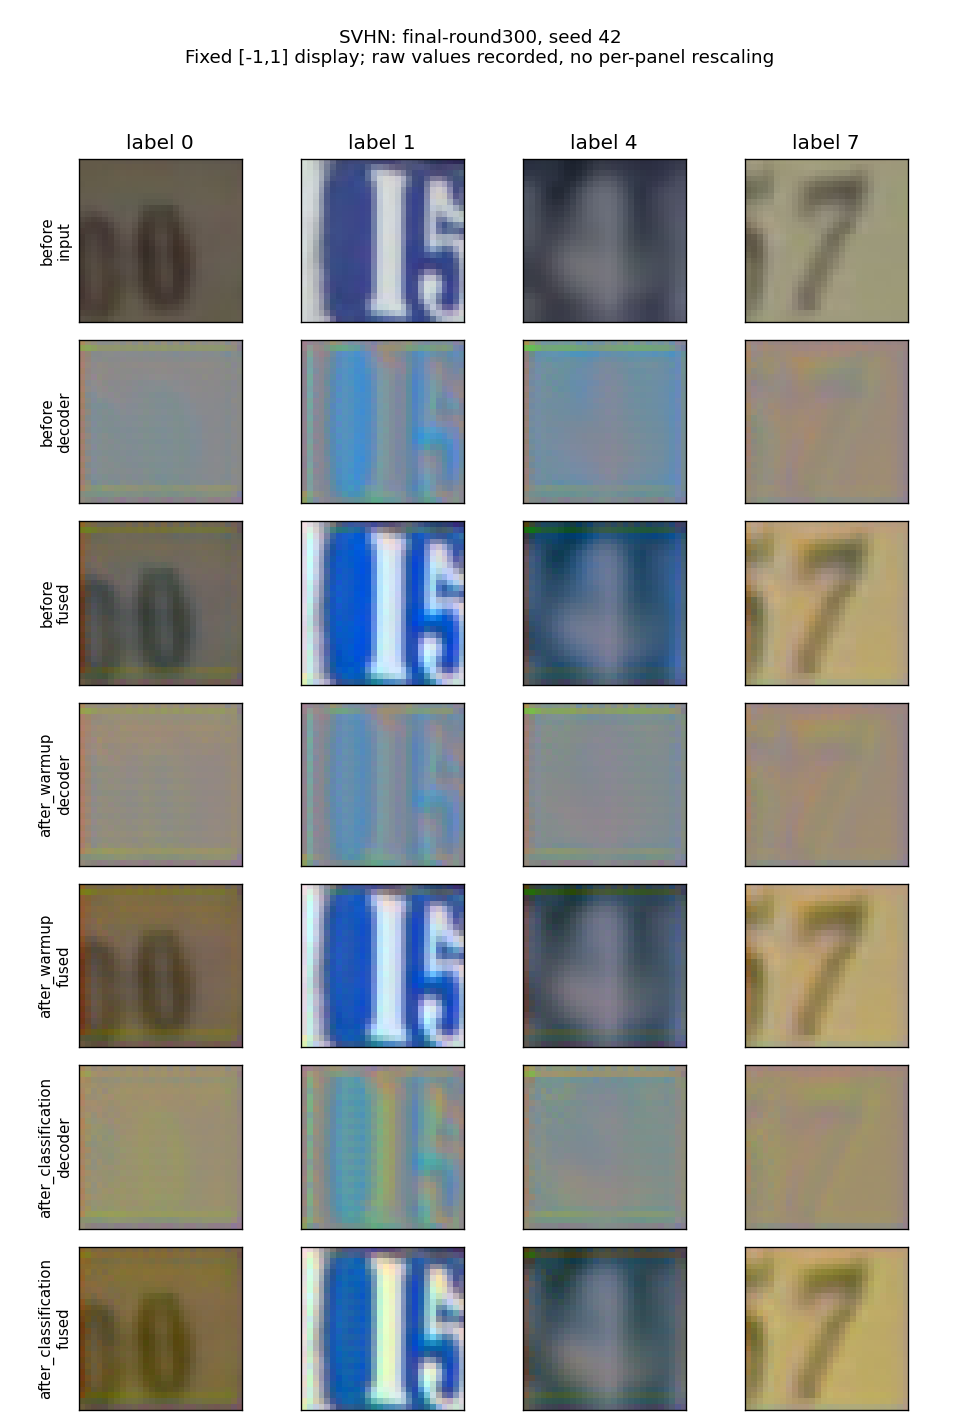
\includegraphics[width=.56in,trim=47.4bp 554.4bp 430.2bp 204.0bp,clip]{figures/digits/final-round300-SVHN.png} & 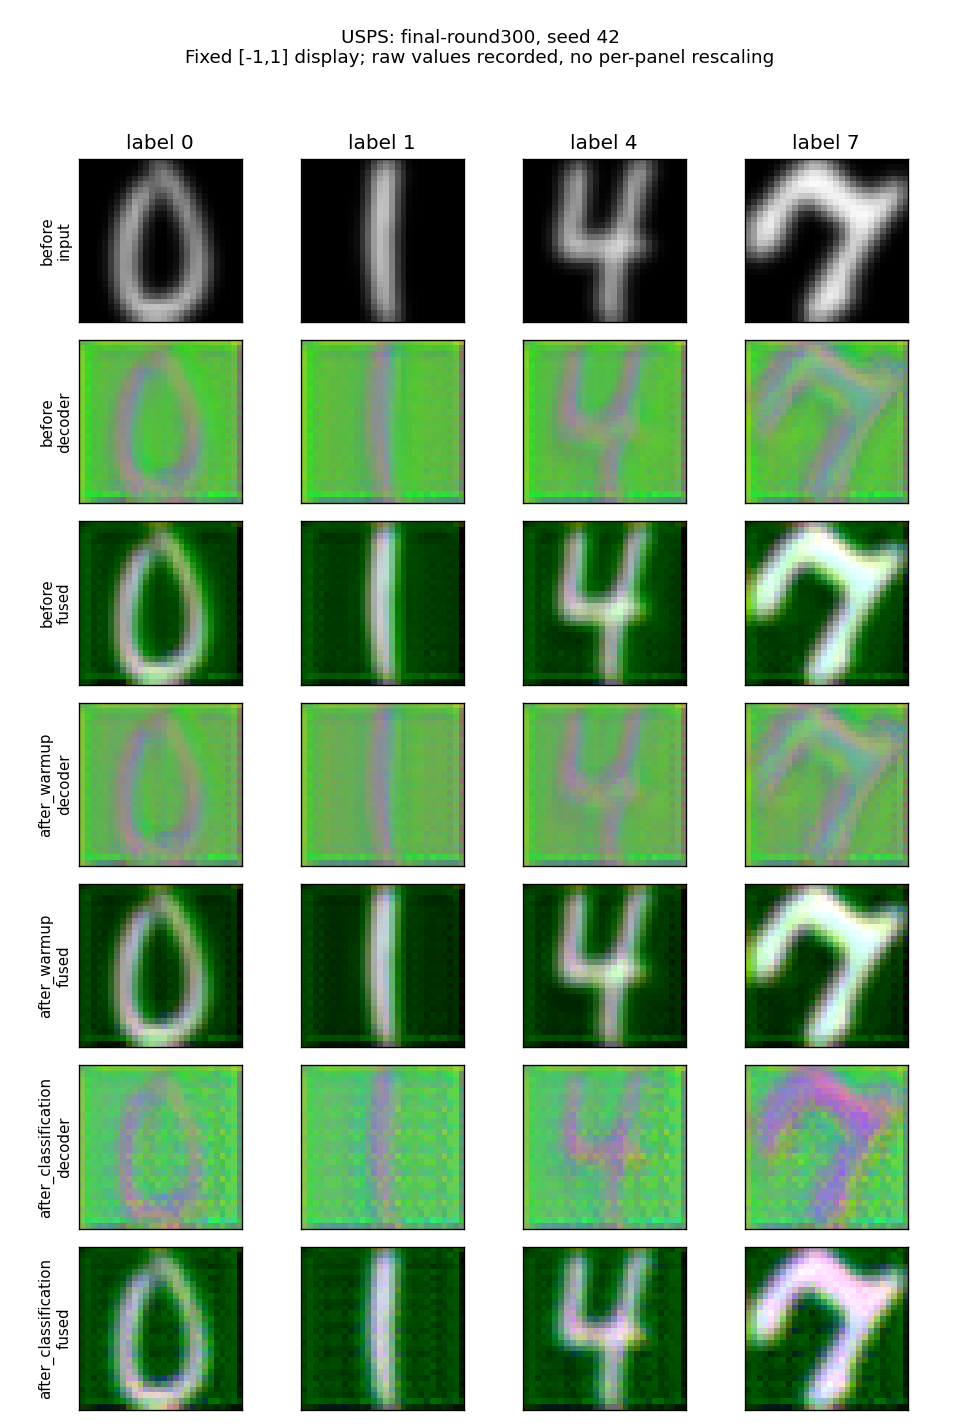
\includegraphics[width=.56in,trim=47.4bp 554.4bp 430.2bp 204.0bp,clip]{figures/digits/final-round300-USPS.png} & 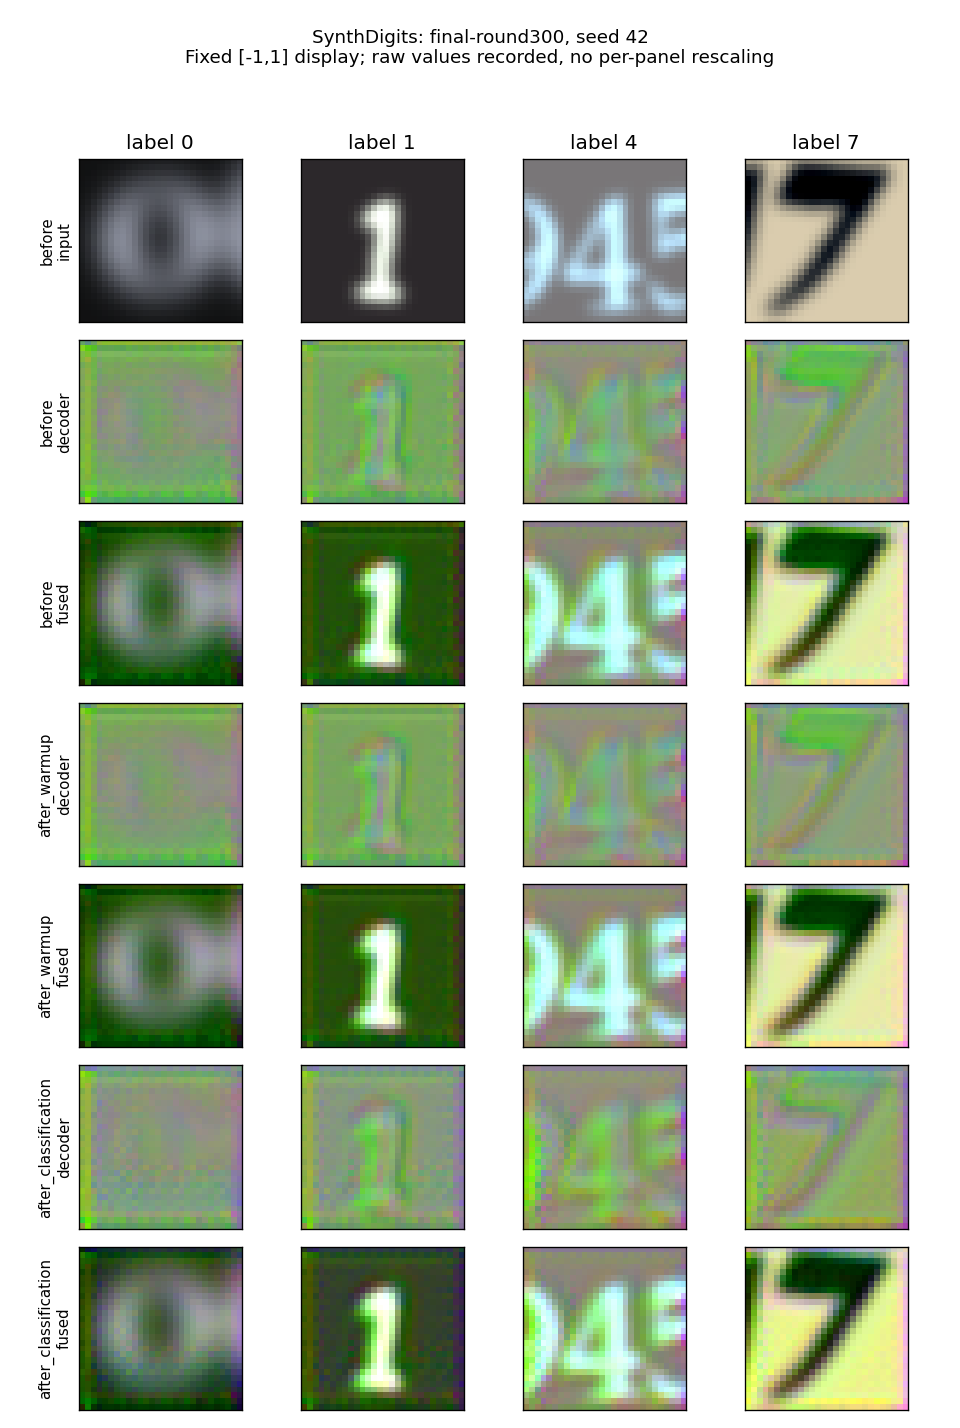
\includegraphics[width=.56in,trim=47.4bp 554.4bp 430.2bp 204.0bp,clip]{figures/digits/final-round300-SynthDigits.png} & 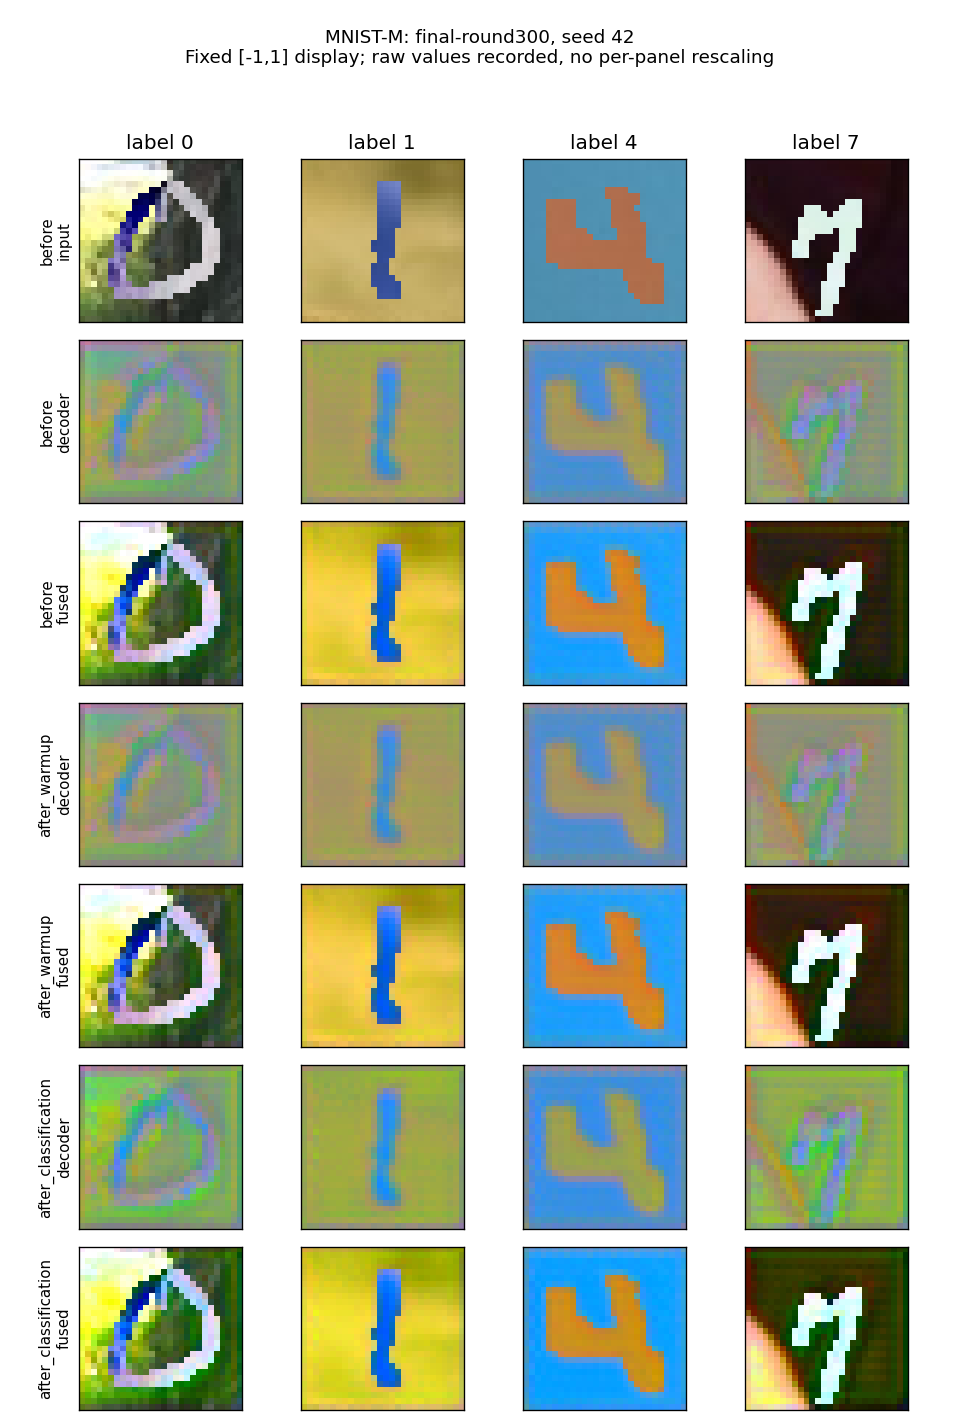
\includegraphics[width=.56in,trim=47.4bp 554.4bp 430.2bp 204.0bp,clip]{figures/digits/final-round300-MNIST-M.png} \\[-2pt]
\raisebox{.20in}{\scriptsize\shortstack[r]{Before\\fused}} & 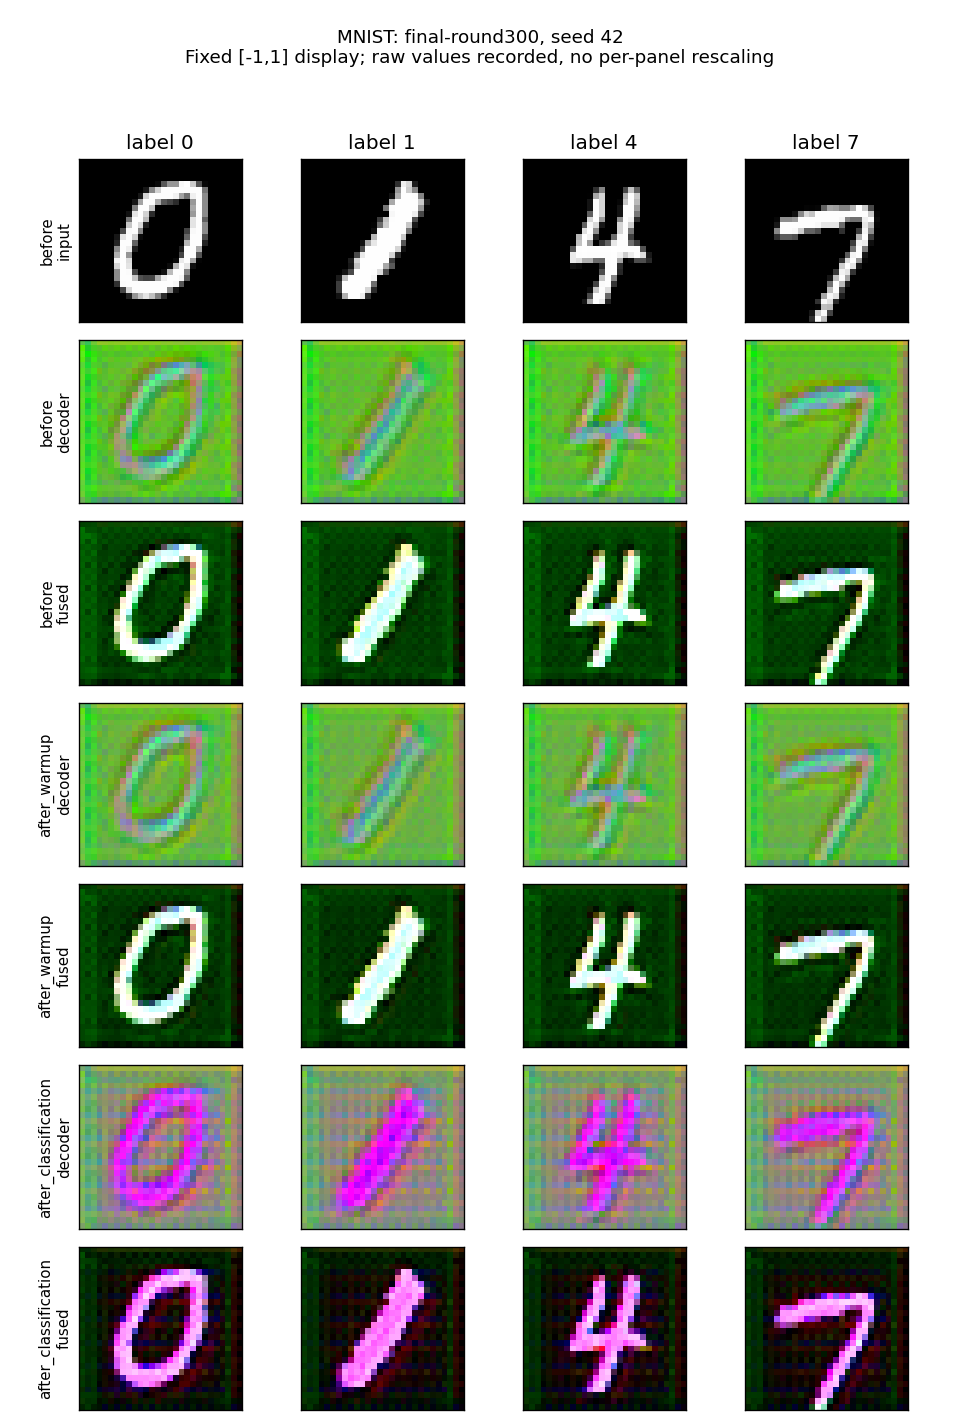
\includegraphics[width=.56in,trim=47.4bp 445.2bp 430.2bp 313.2bp,clip]{figures/digits/final-round300-MNIST.png} & 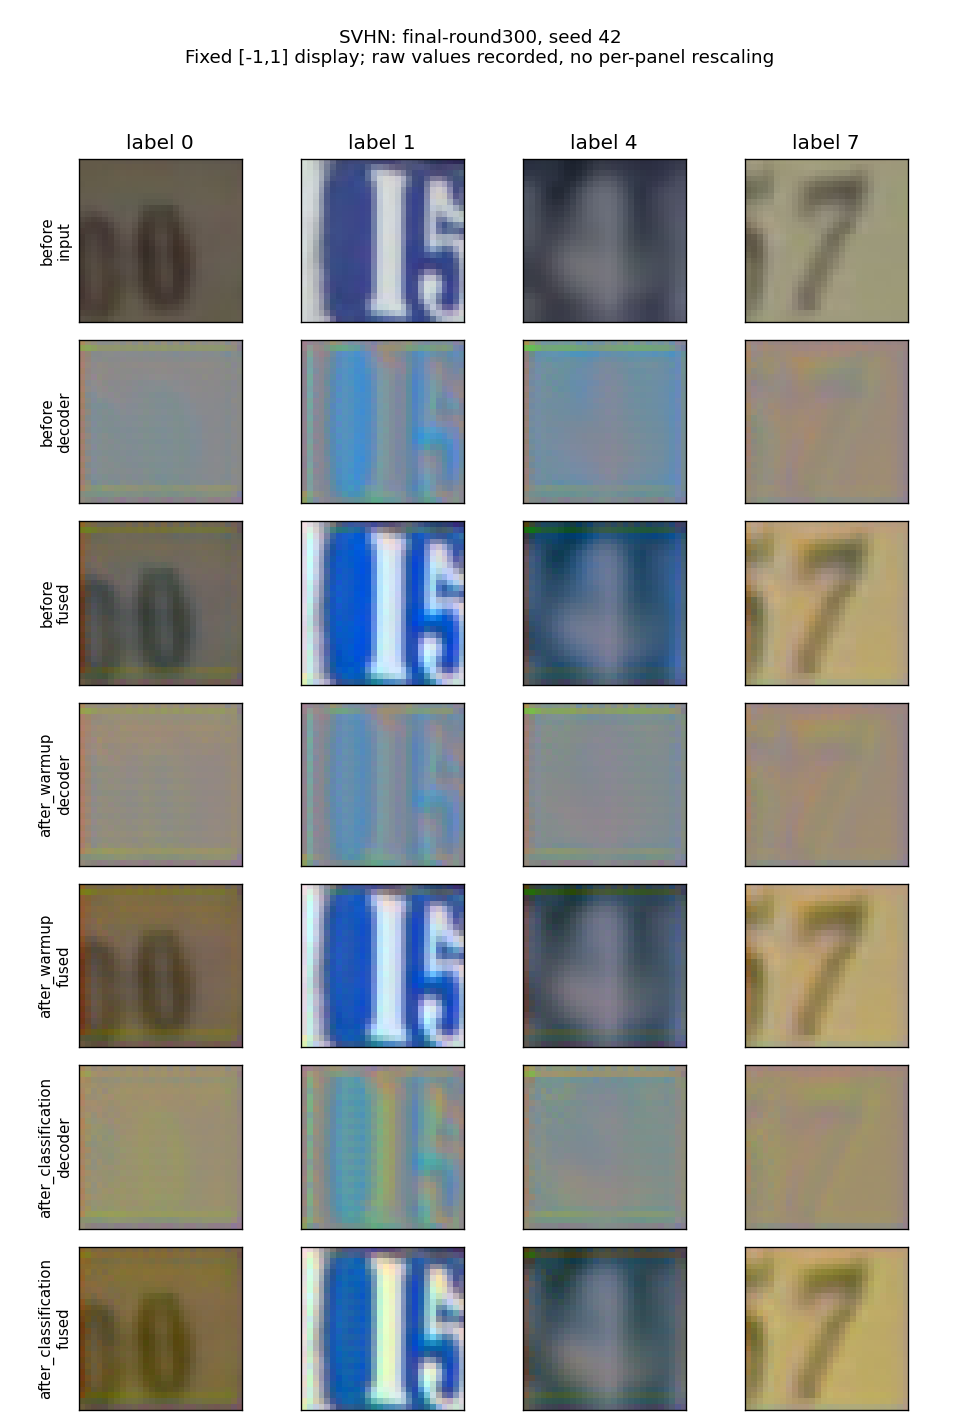
\includegraphics[width=.56in,trim=47.4bp 445.2bp 430.2bp 313.2bp,clip]{figures/digits/final-round300-SVHN.png} & 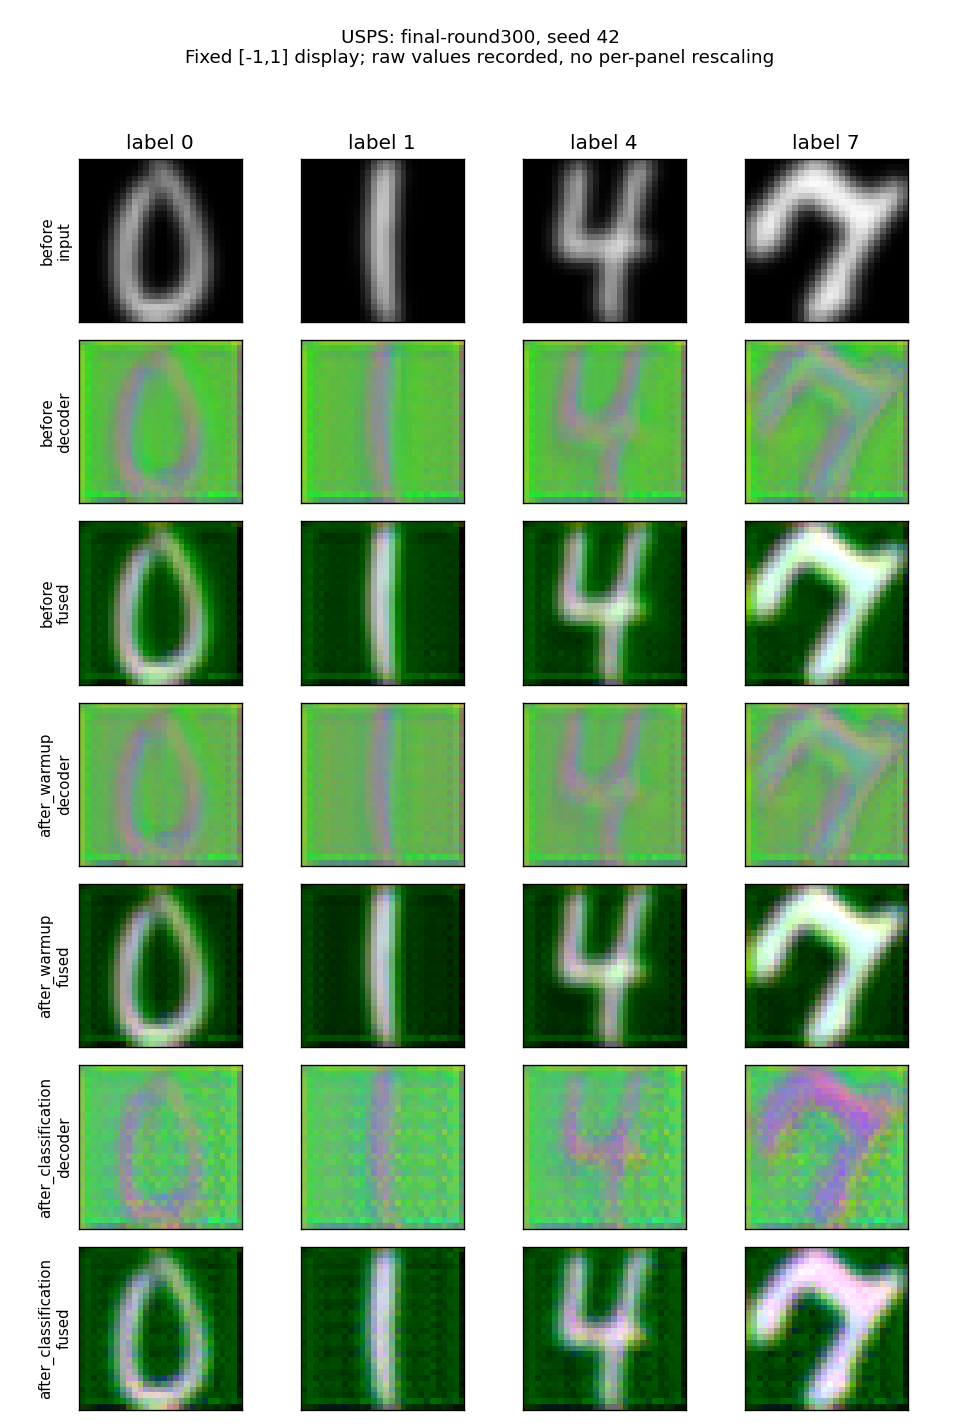
\includegraphics[width=.56in,trim=47.4bp 445.2bp 430.2bp 313.2bp,clip]{figures/digits/final-round300-USPS.png} & 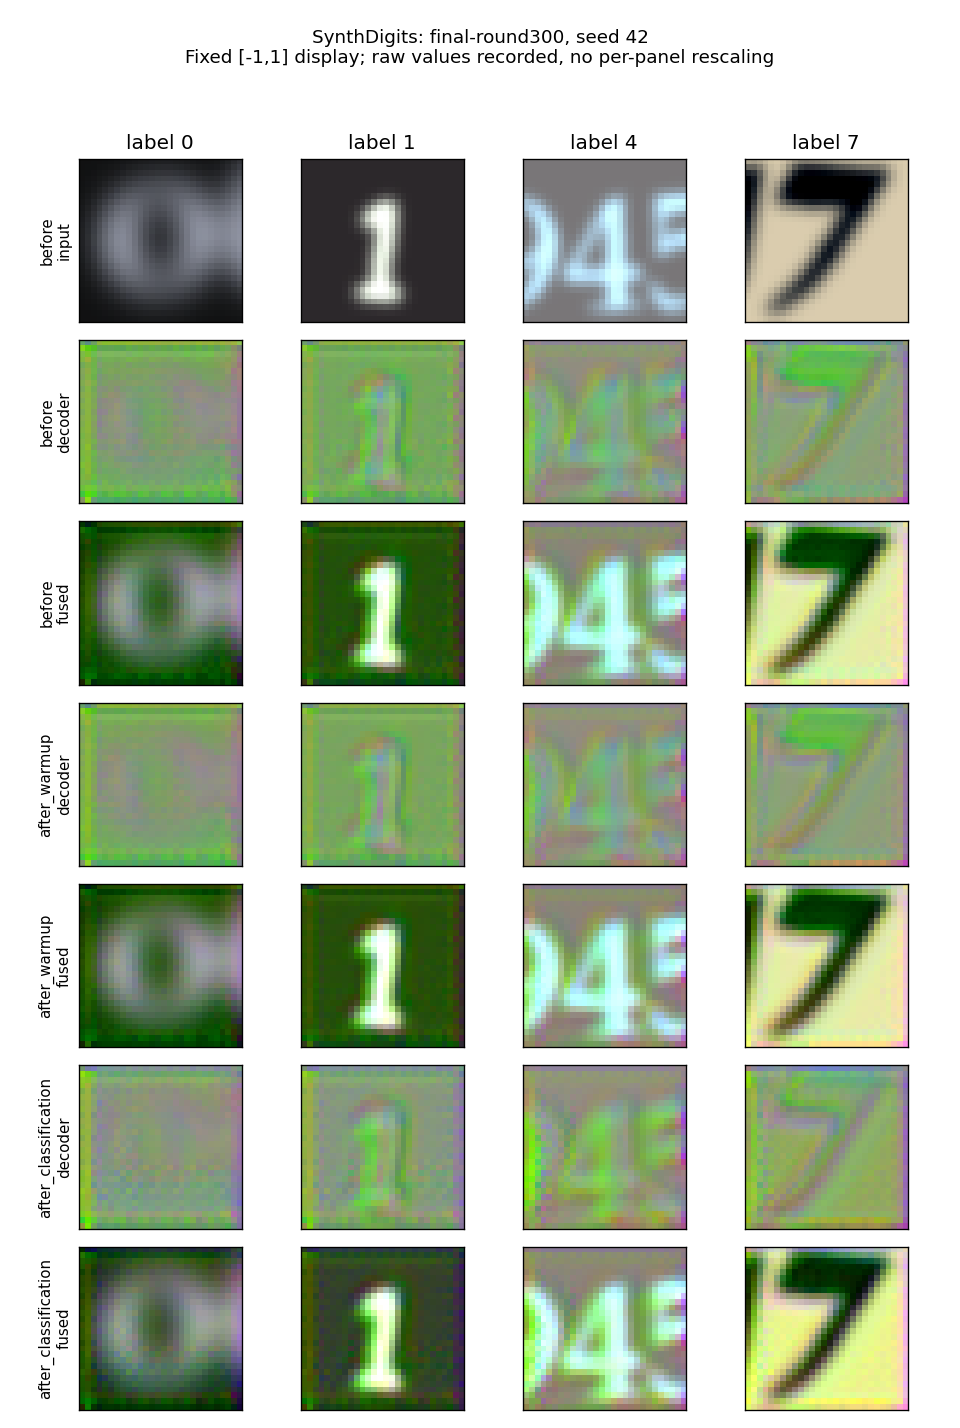
\includegraphics[width=.56in,trim=47.4bp 445.2bp 430.2bp 313.2bp,clip]{figures/digits/final-round300-SynthDigits.png} & 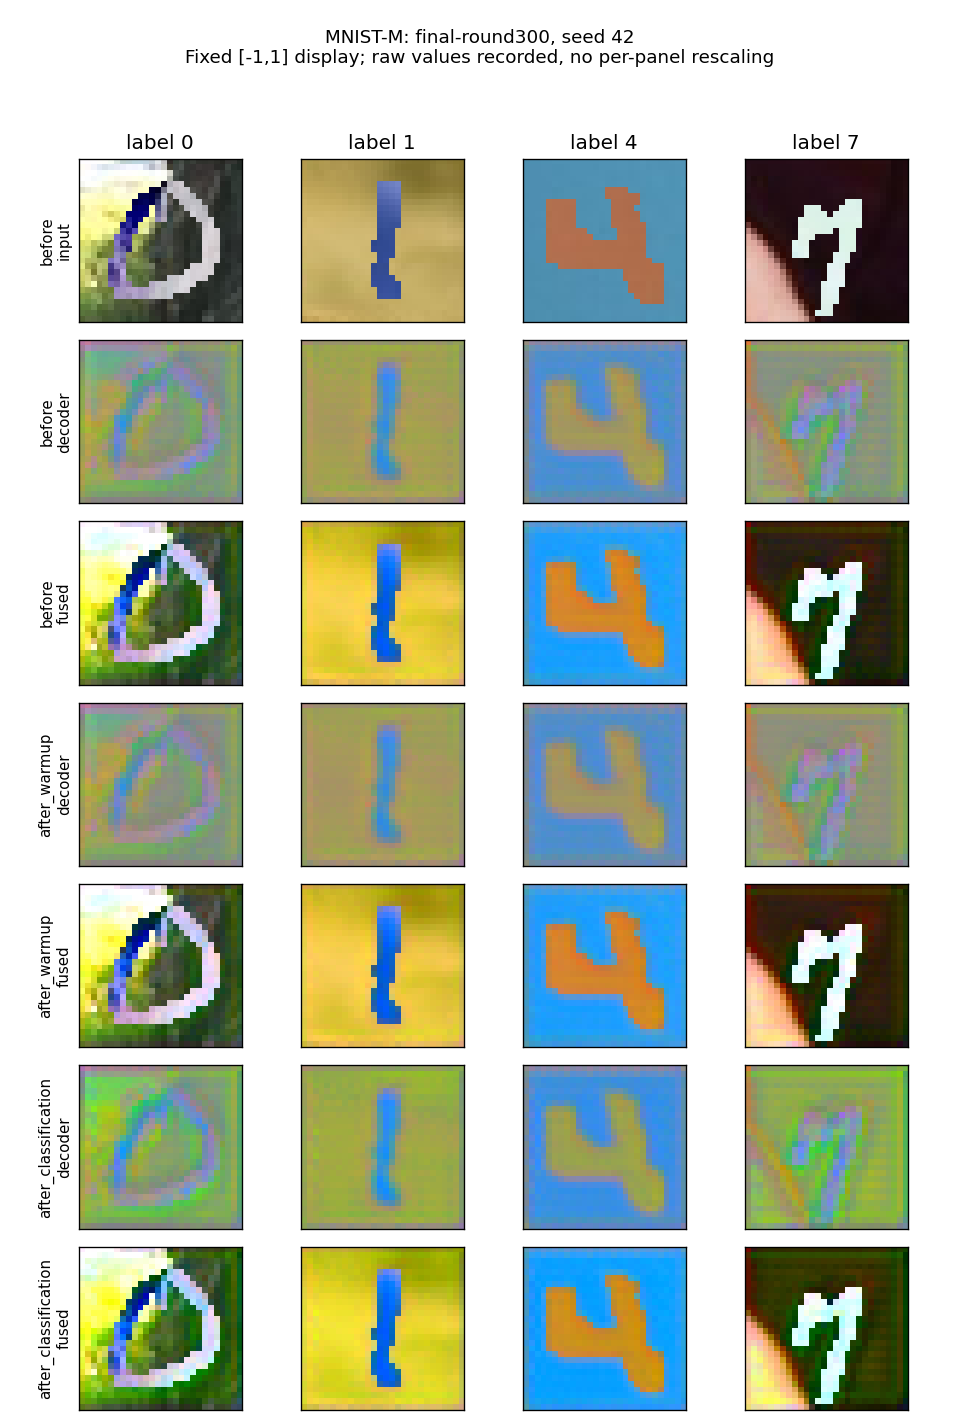
\includegraphics[width=.56in,trim=47.4bp 445.2bp 430.2bp 313.2bp,clip]{figures/digits/final-round300-MNIST-M.png} \\[-2pt]
\raisebox{.20in}{\scriptsize\shortstack[r]{After warm-up\\decoder}} & 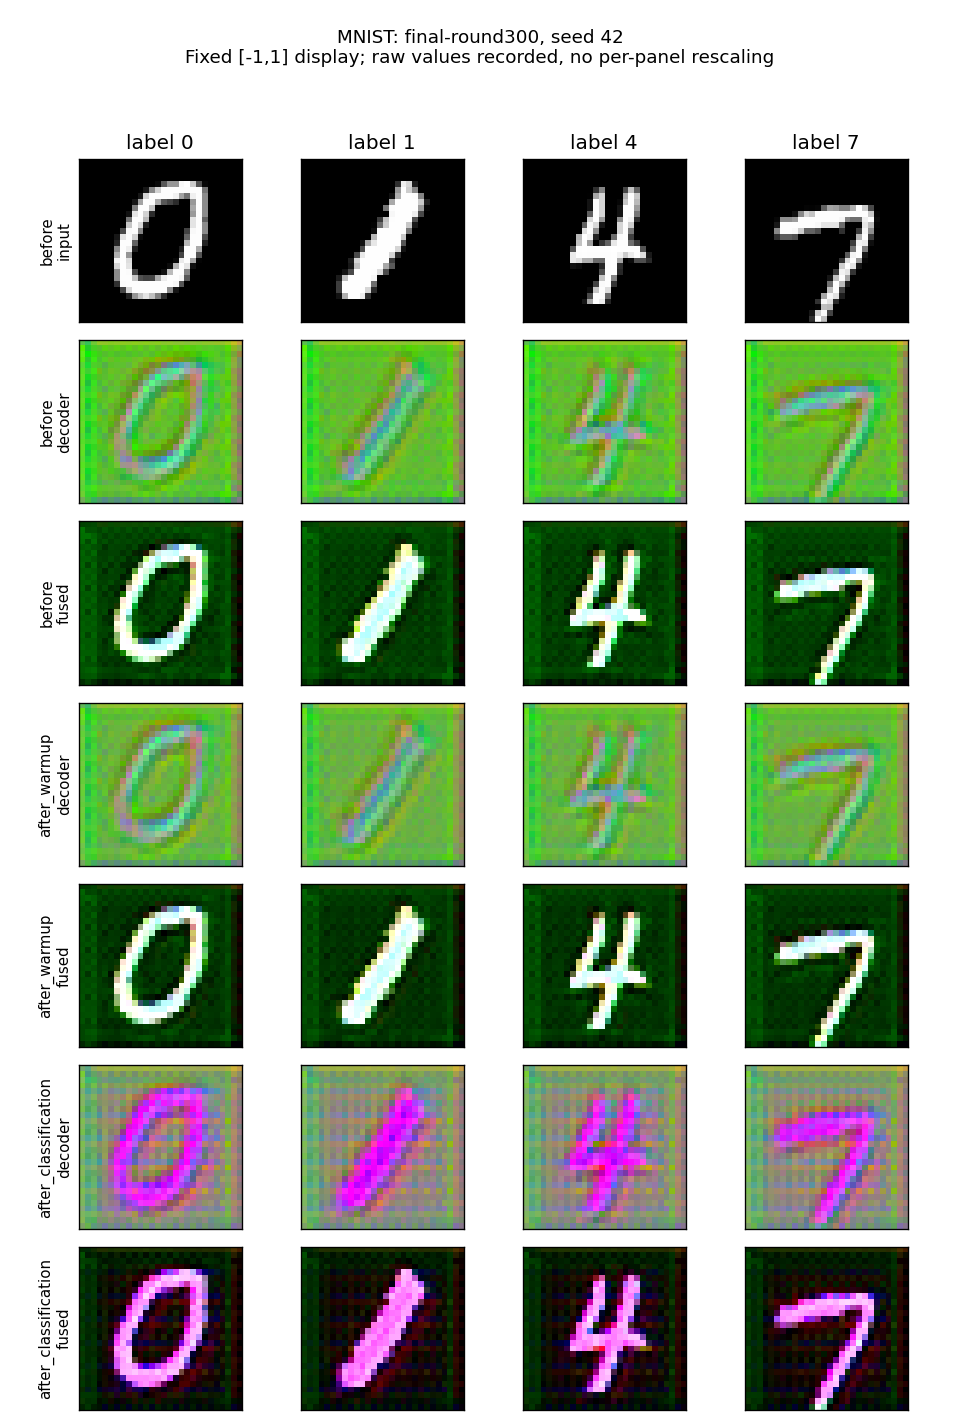
\includegraphics[width=.56in,trim=47.4bp 336.0bp 430.2bp 422.4bp,clip]{figures/digits/final-round300-MNIST.png} & 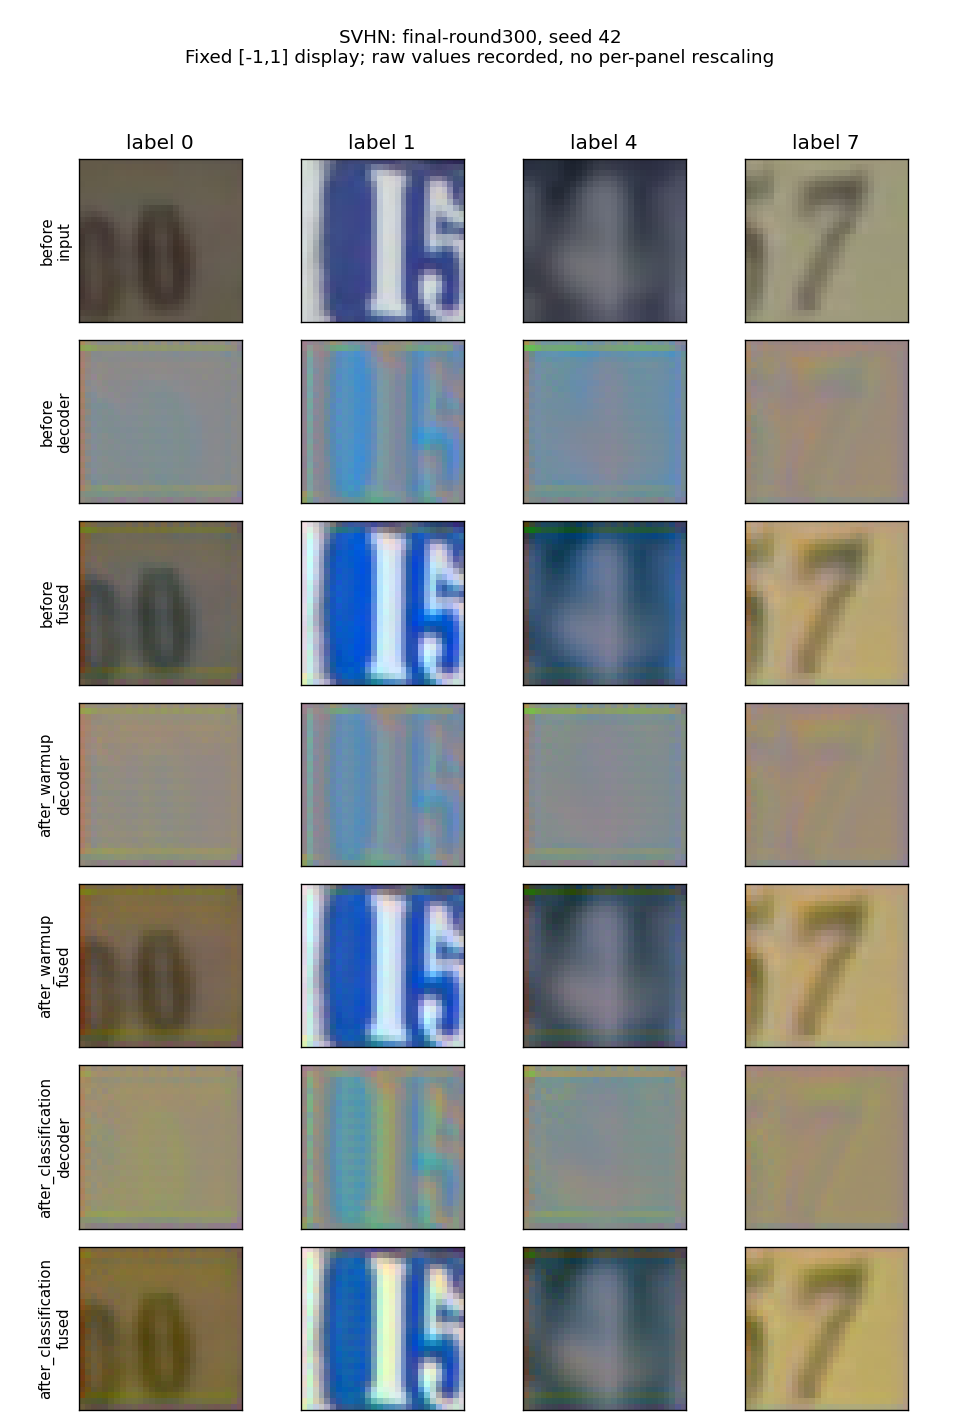
\includegraphics[width=.56in,trim=47.4bp 336.0bp 430.2bp 422.4bp,clip]{figures/digits/final-round300-SVHN.png} & 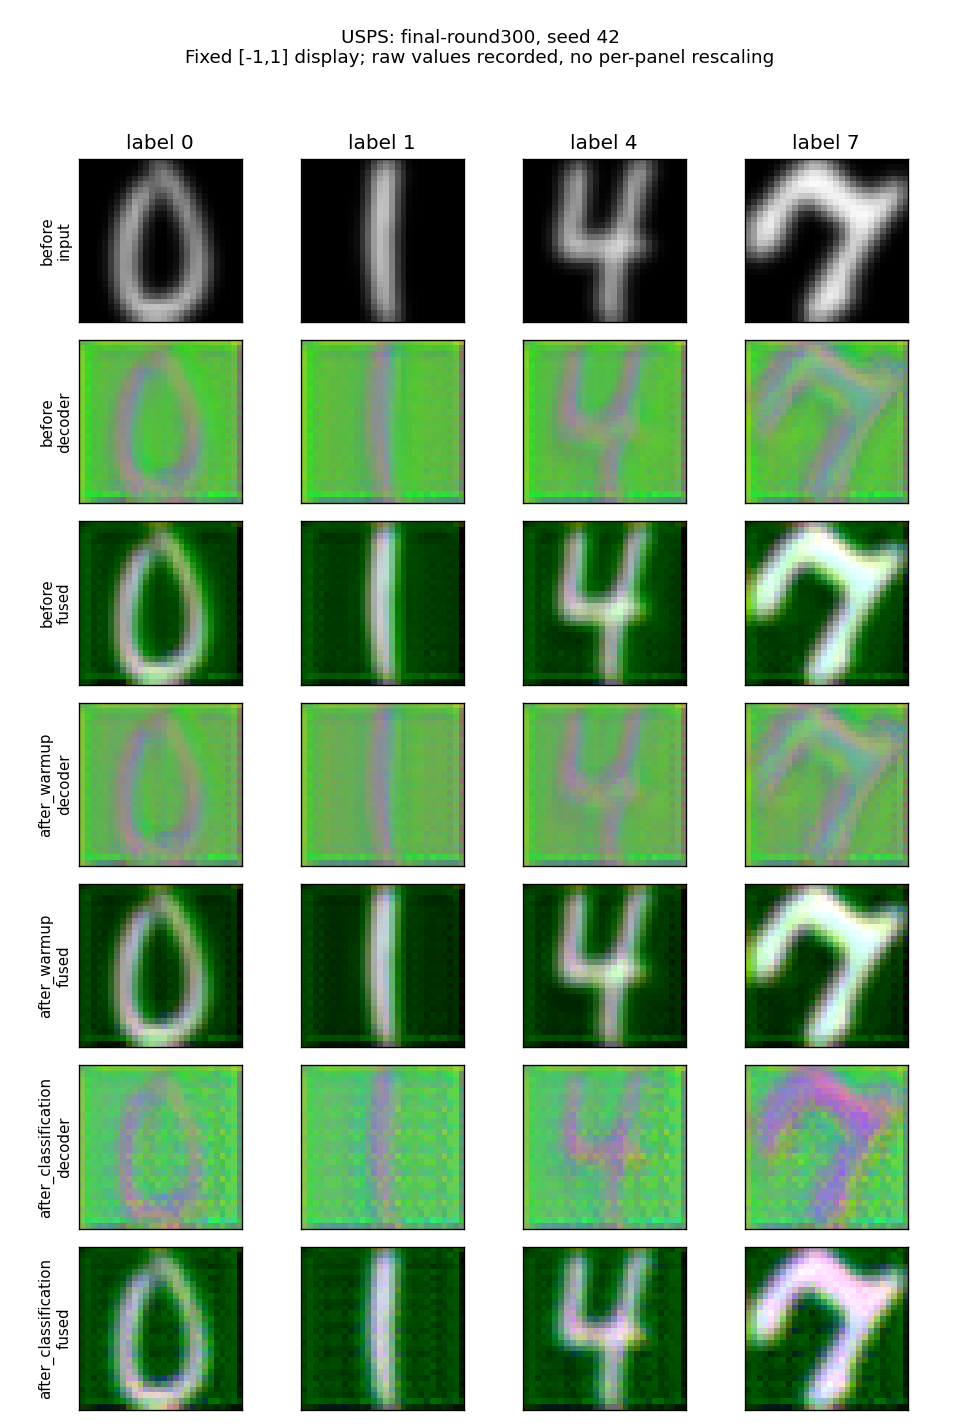
\includegraphics[width=.56in,trim=47.4bp 336.0bp 430.2bp 422.4bp,clip]{figures/digits/final-round300-USPS.png} & 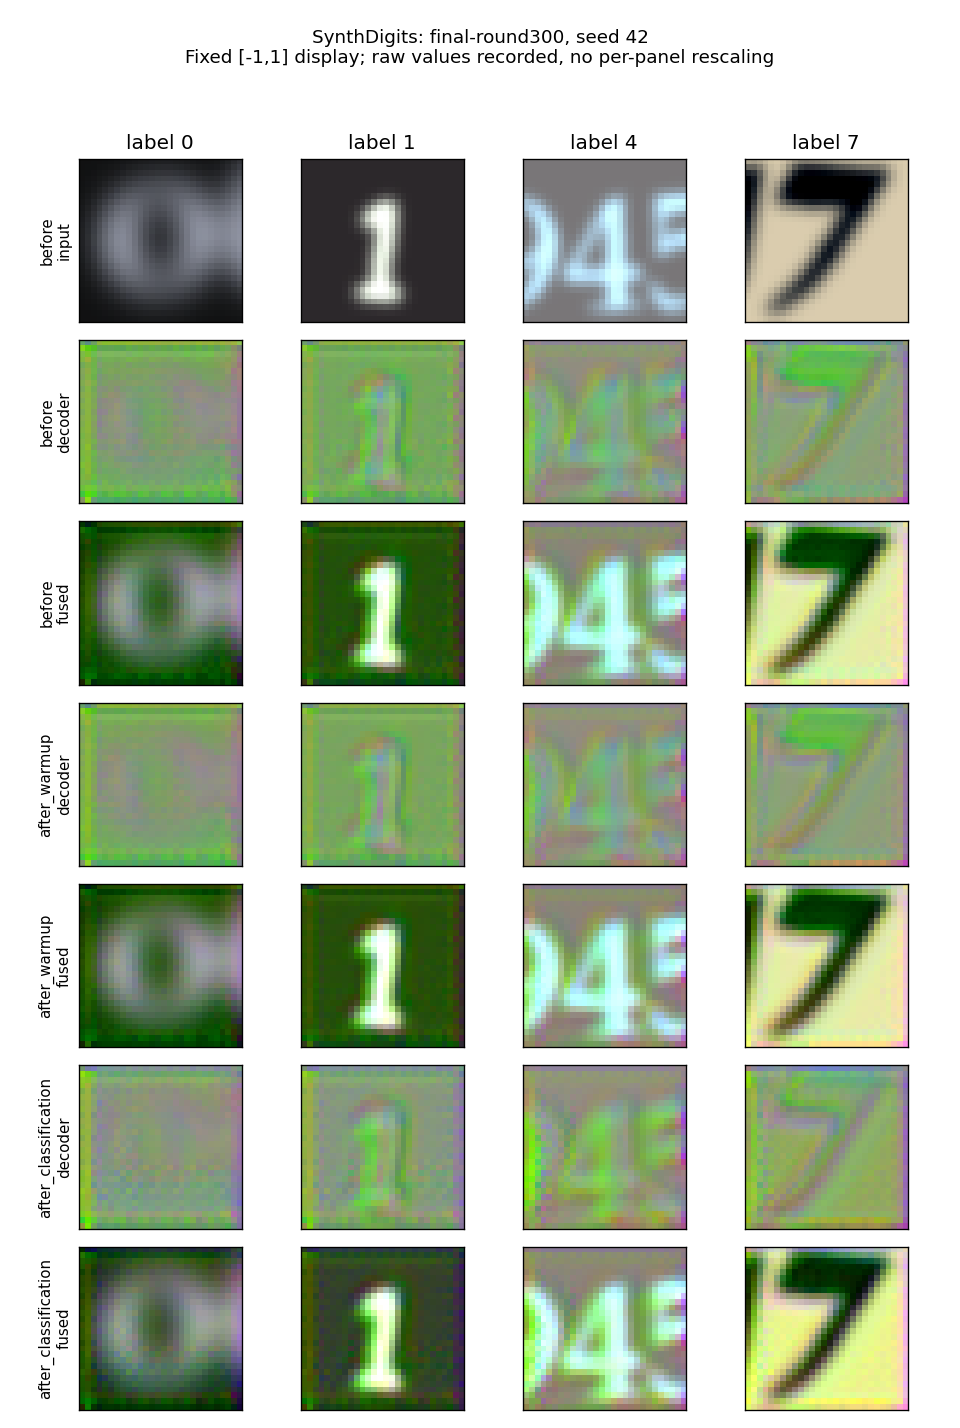
\includegraphics[width=.56in,trim=47.4bp 336.0bp 430.2bp 422.4bp,clip]{figures/digits/final-round300-SynthDigits.png} & 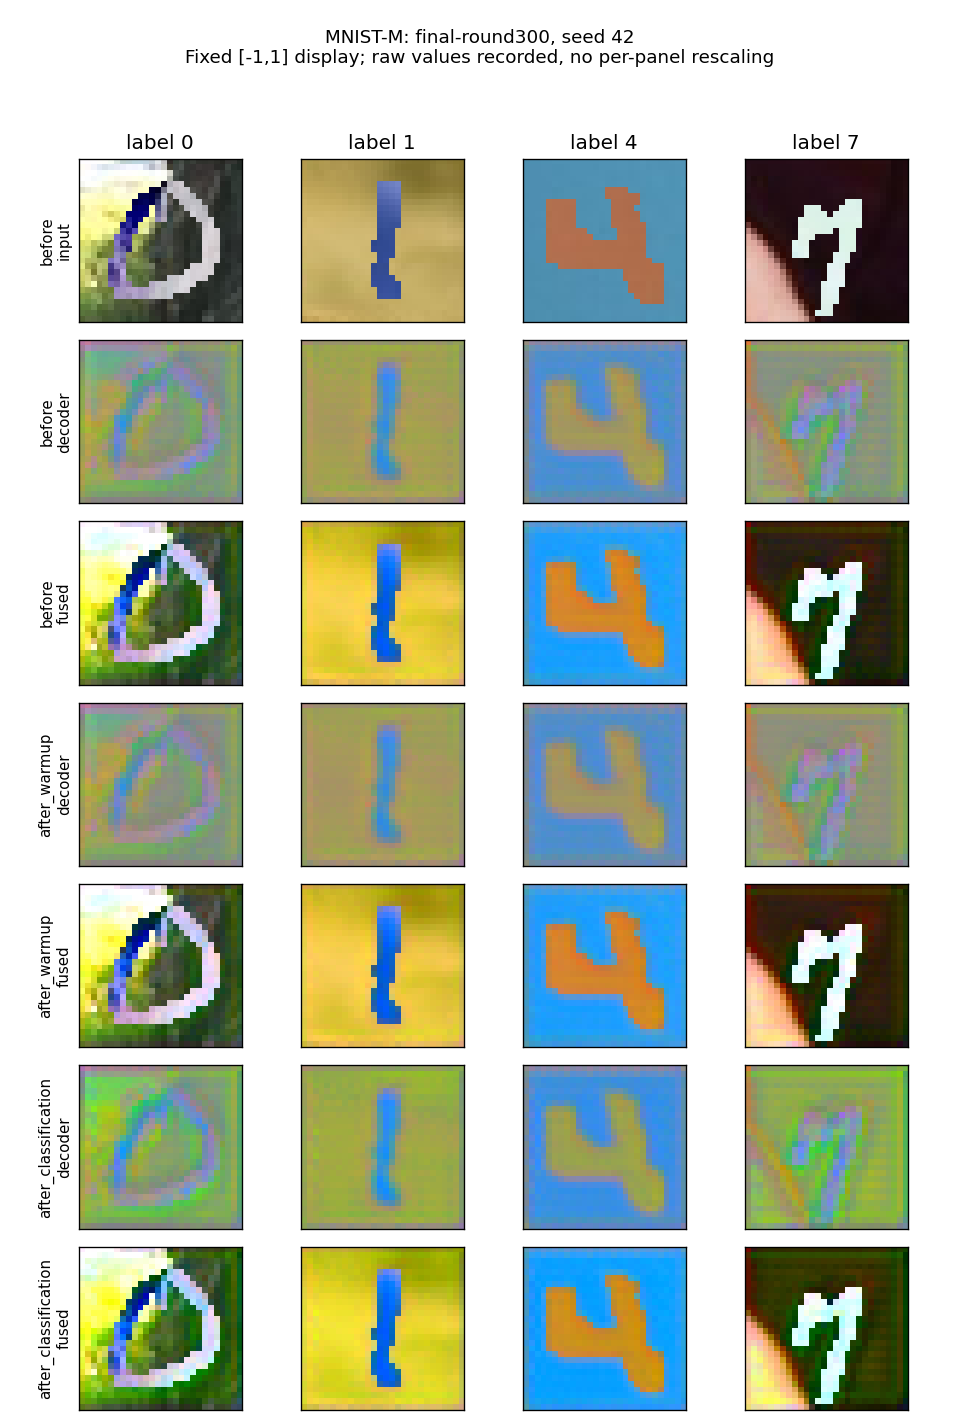
\includegraphics[width=.56in,trim=47.4bp 336.0bp 430.2bp 422.4bp,clip]{figures/digits/final-round300-MNIST-M.png} \\[-2pt]
\raisebox{.20in}{\scriptsize\shortstack[r]{After warm-up\\fused}} & 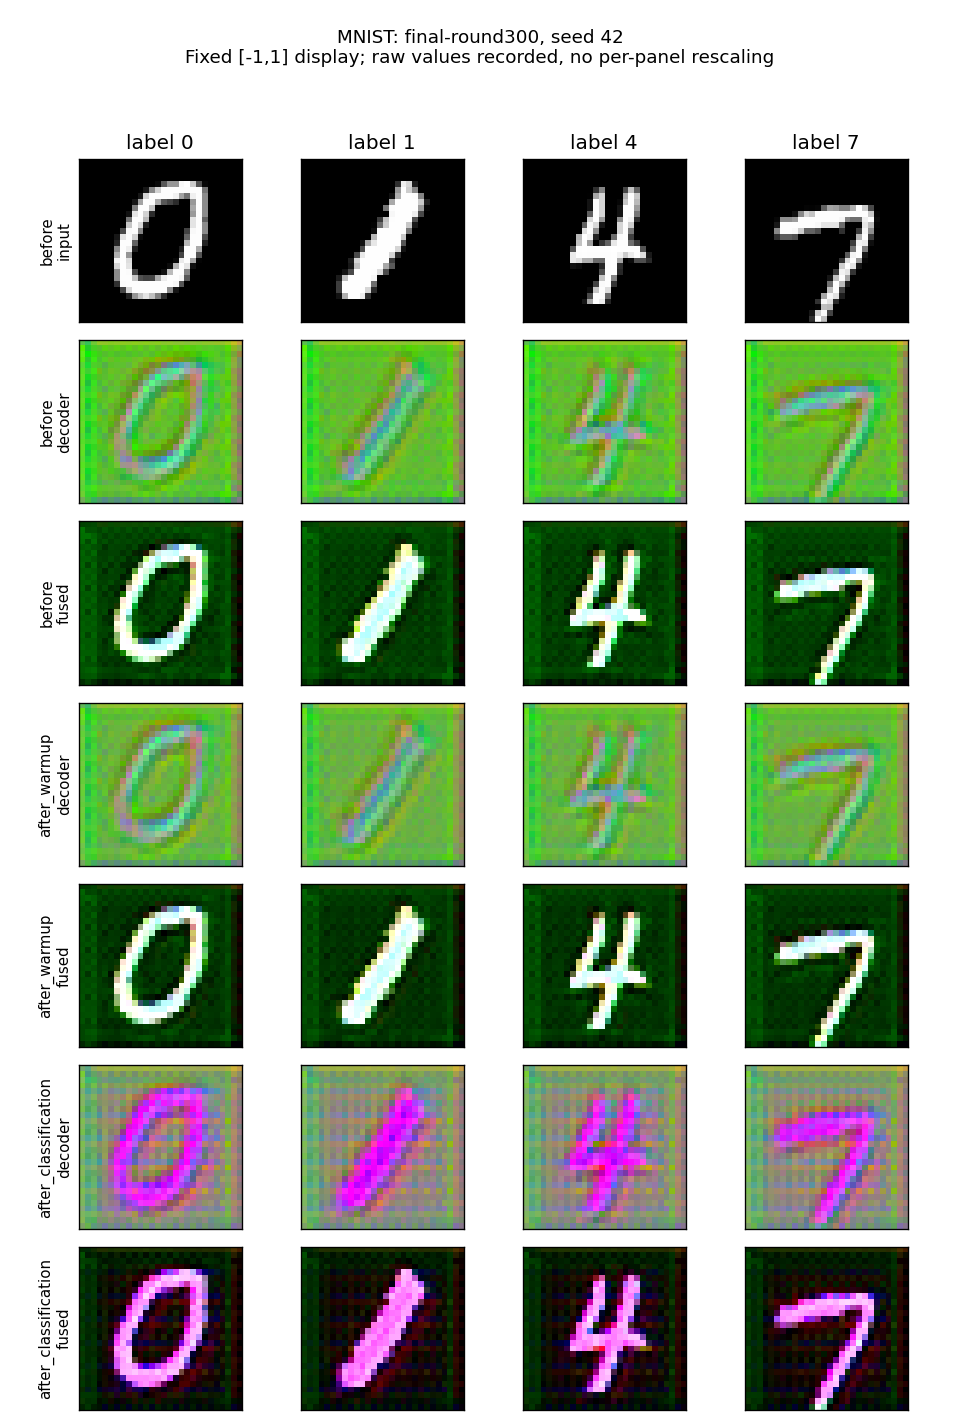
\includegraphics[width=.56in,trim=47.4bp 227.4bp 430.2bp 531.0bp,clip]{figures/digits/final-round300-MNIST.png} & 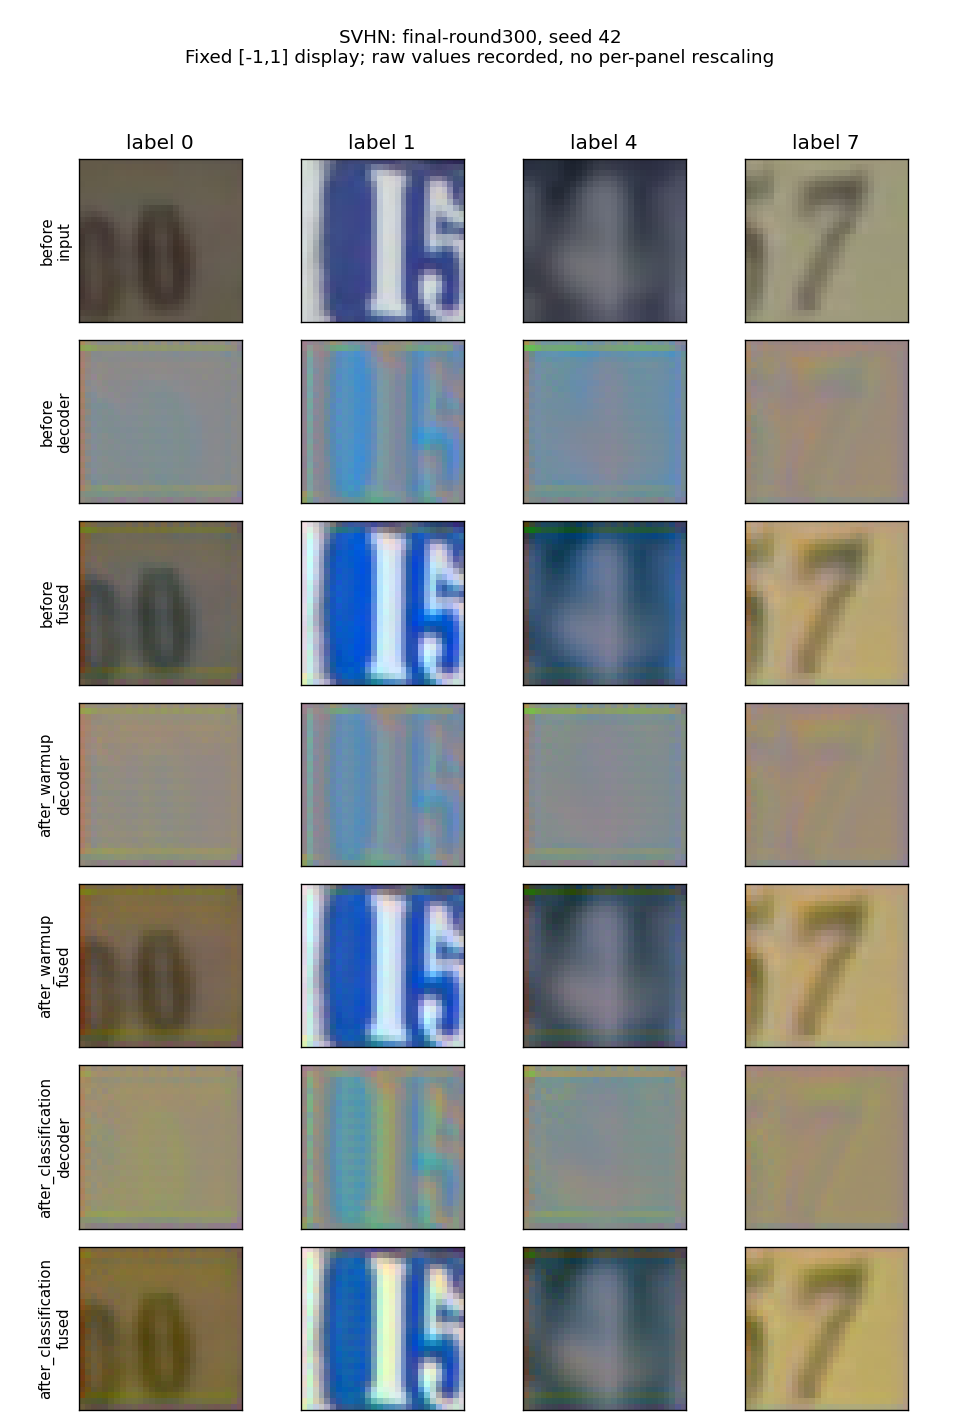
\includegraphics[width=.56in,trim=47.4bp 227.4bp 430.2bp 531.0bp,clip]{figures/digits/final-round300-SVHN.png} & 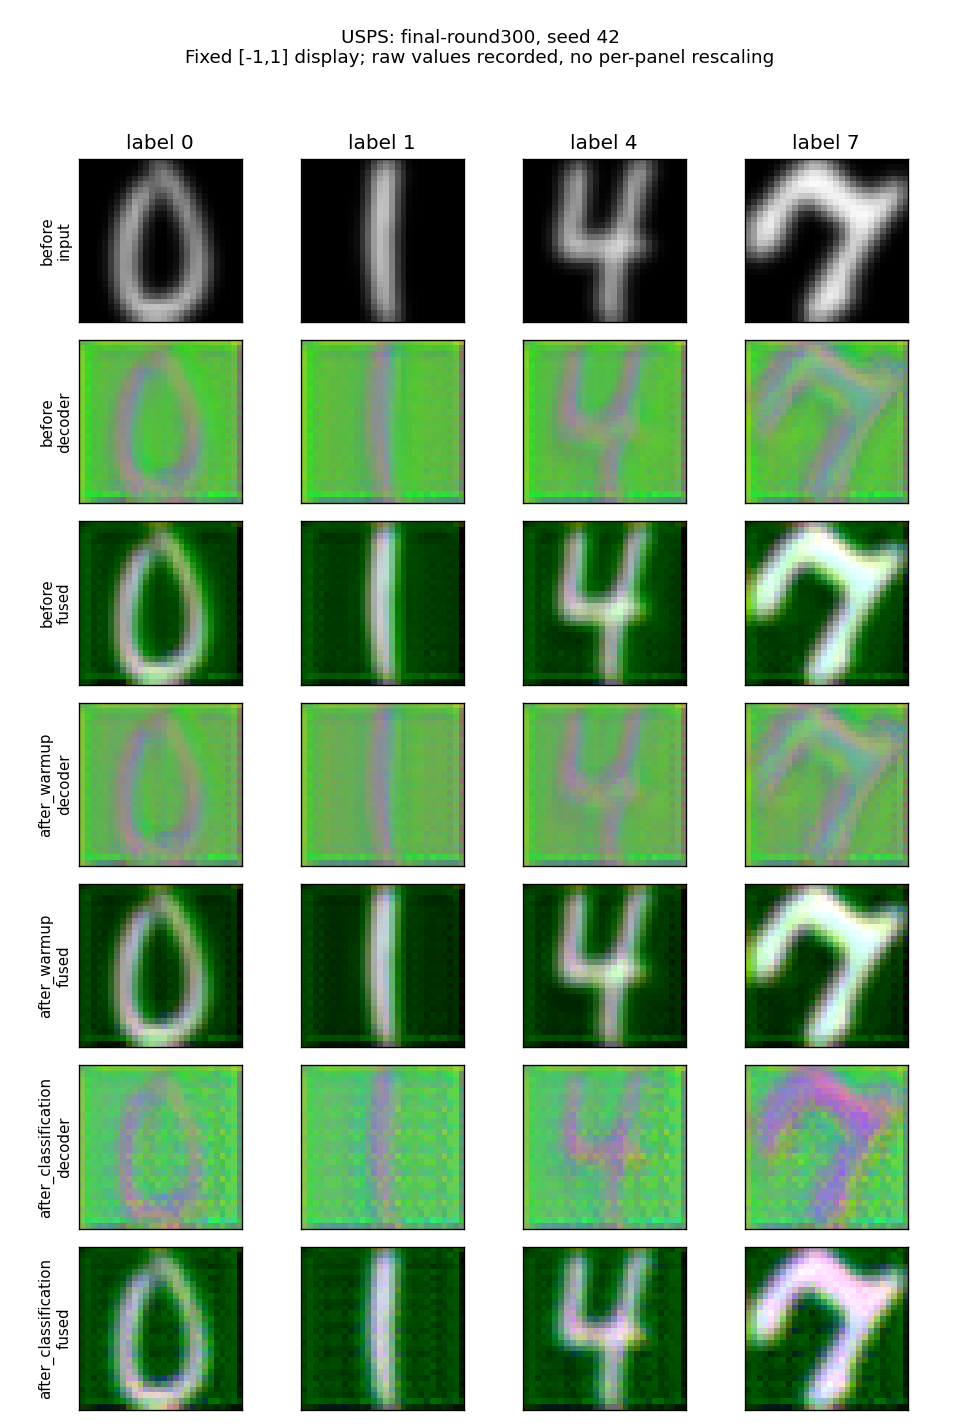
\includegraphics[width=.56in,trim=47.4bp 227.4bp 430.2bp 531.0bp,clip]{figures/digits/final-round300-USPS.png} & 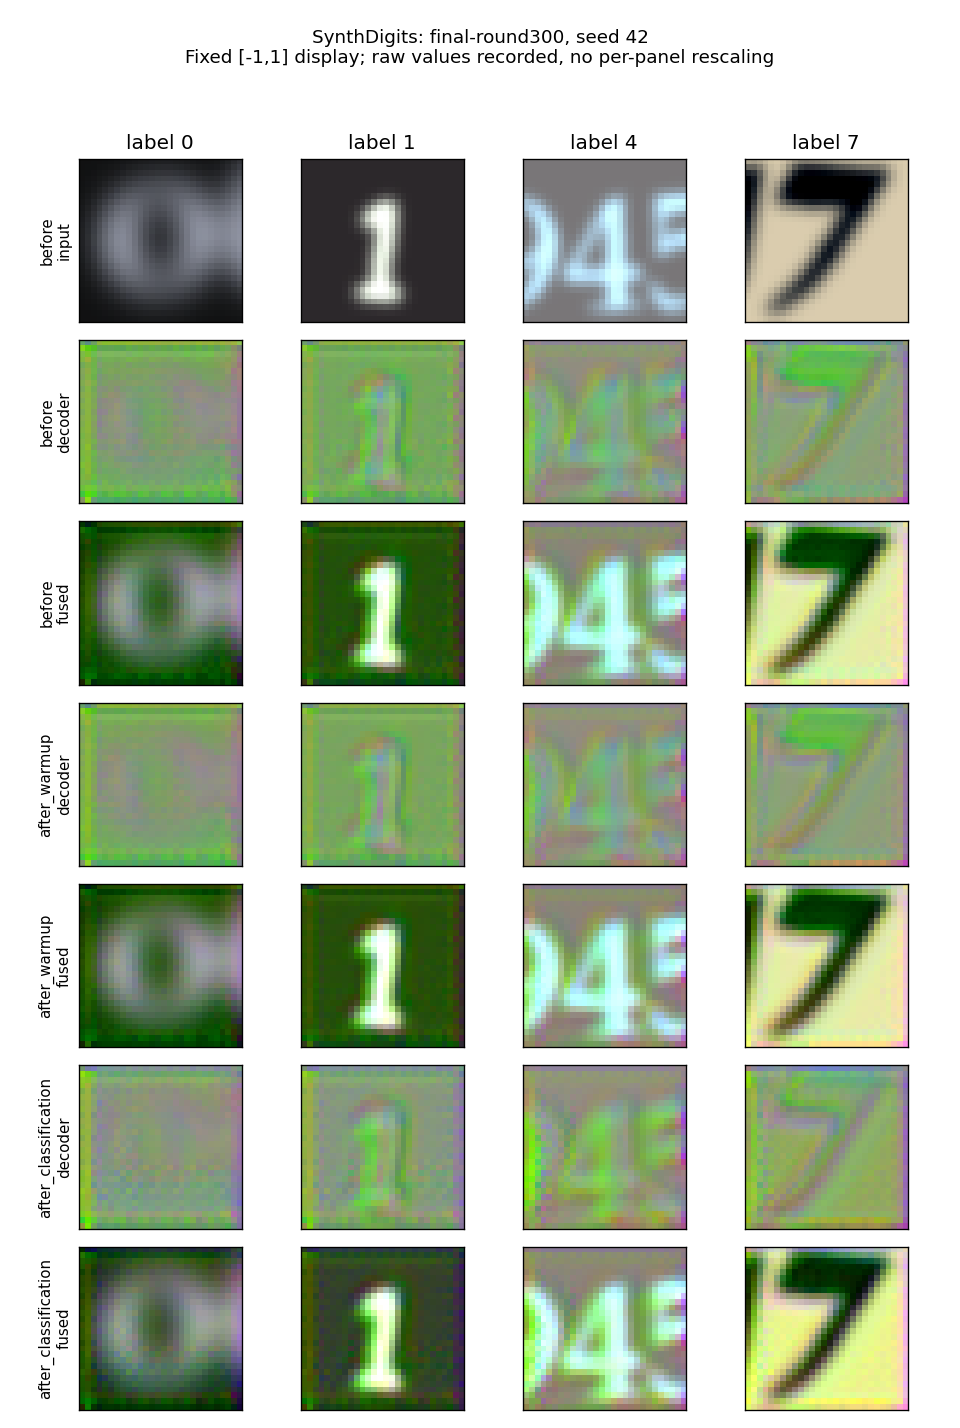
\includegraphics[width=.56in,trim=47.4bp 227.4bp 430.2bp 531.0bp,clip]{figures/digits/final-round300-SynthDigits.png} & 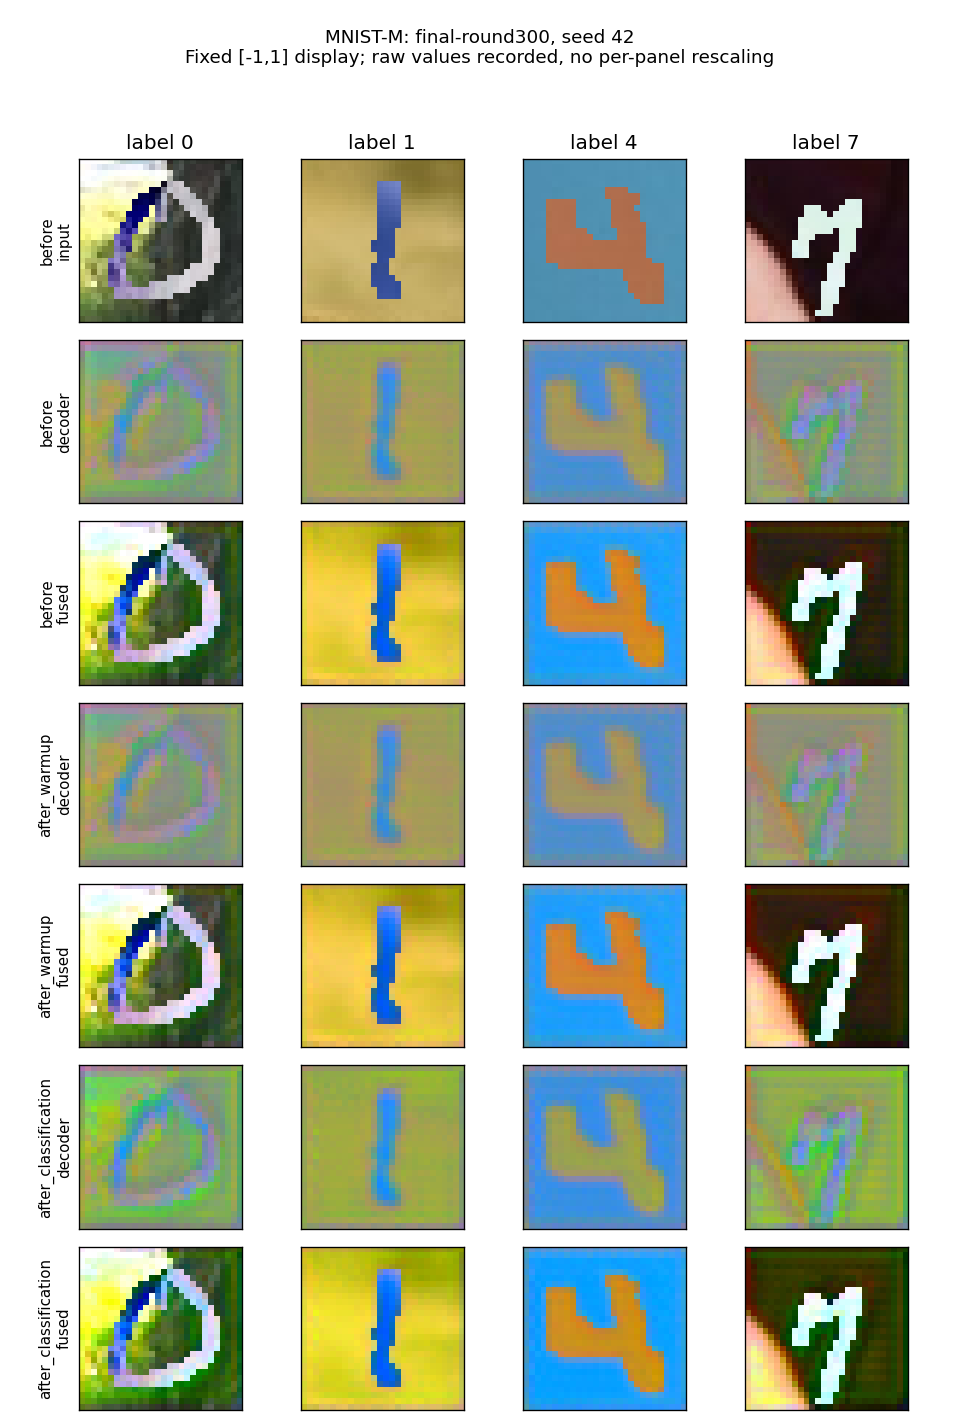
\includegraphics[width=.56in,trim=47.4bp 227.4bp 430.2bp 531.0bp,clip]{figures/digits/final-round300-MNIST-M.png} \\[-2pt]
\raisebox{.20in}{\scriptsize\shortstack[r]{After classification\\decoder}} & 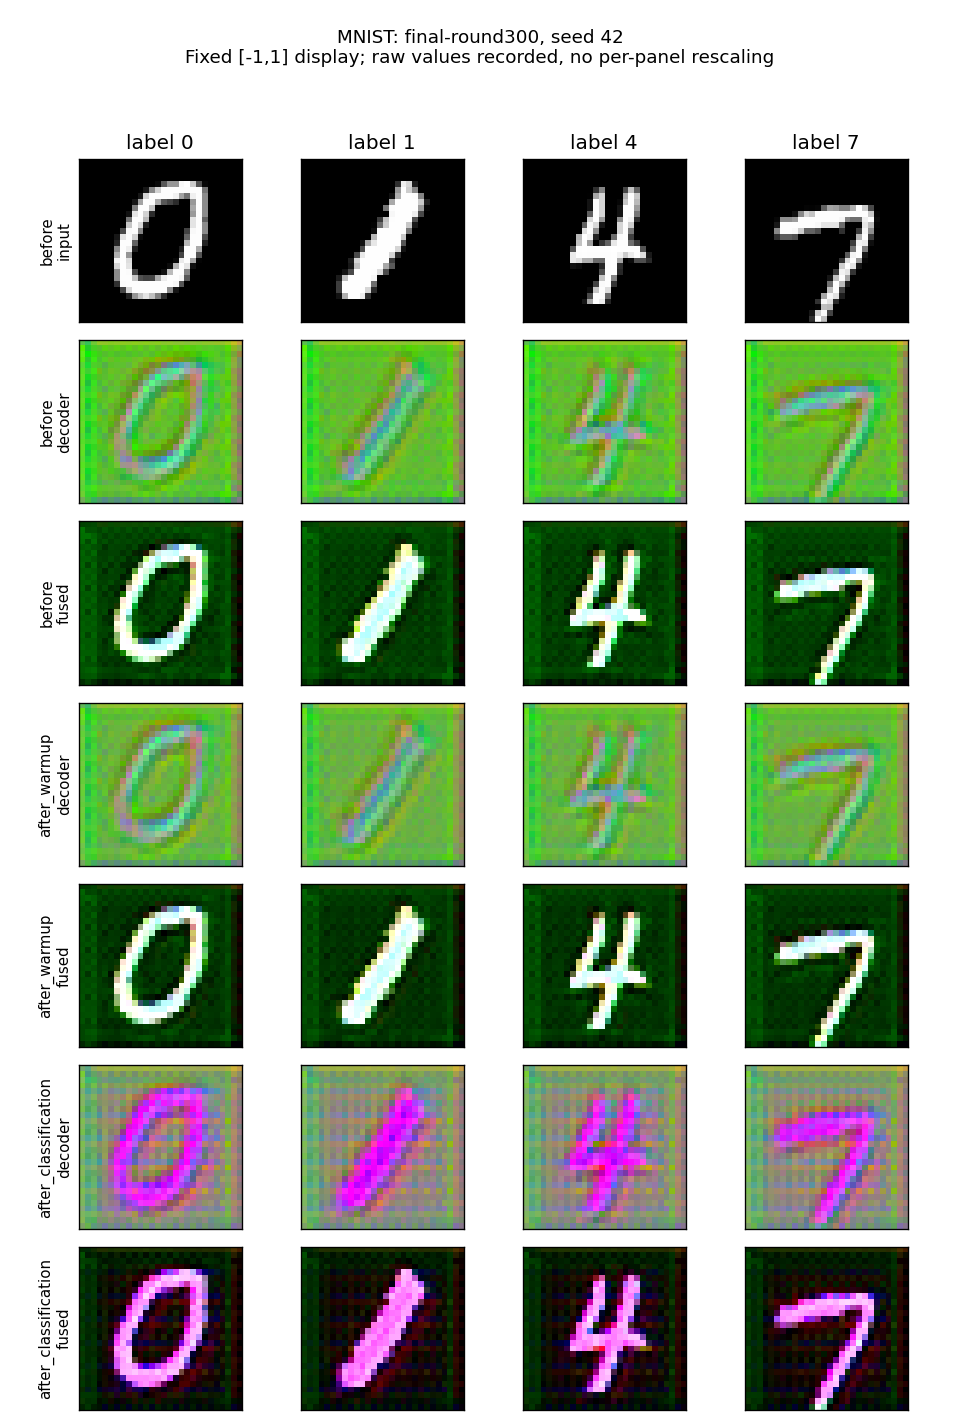
\includegraphics[width=.56in,trim=47.4bp 118.8bp 430.2bp 639.6bp,clip]{figures/digits/final-round300-MNIST.png} & 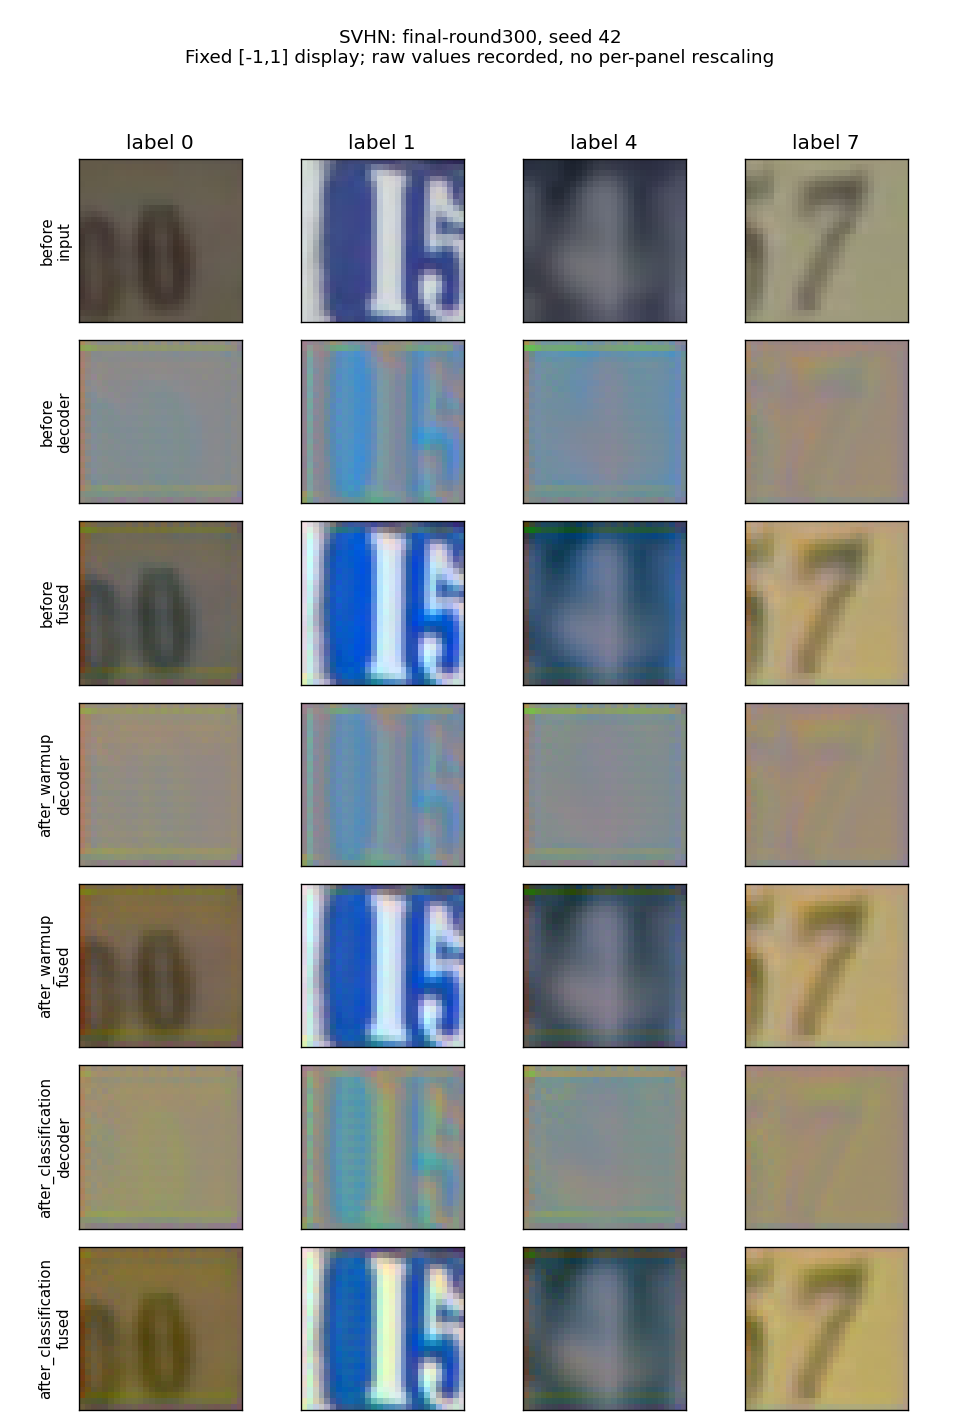
\includegraphics[width=.56in,trim=47.4bp 118.8bp 430.2bp 639.6bp,clip]{figures/digits/final-round300-SVHN.png} & 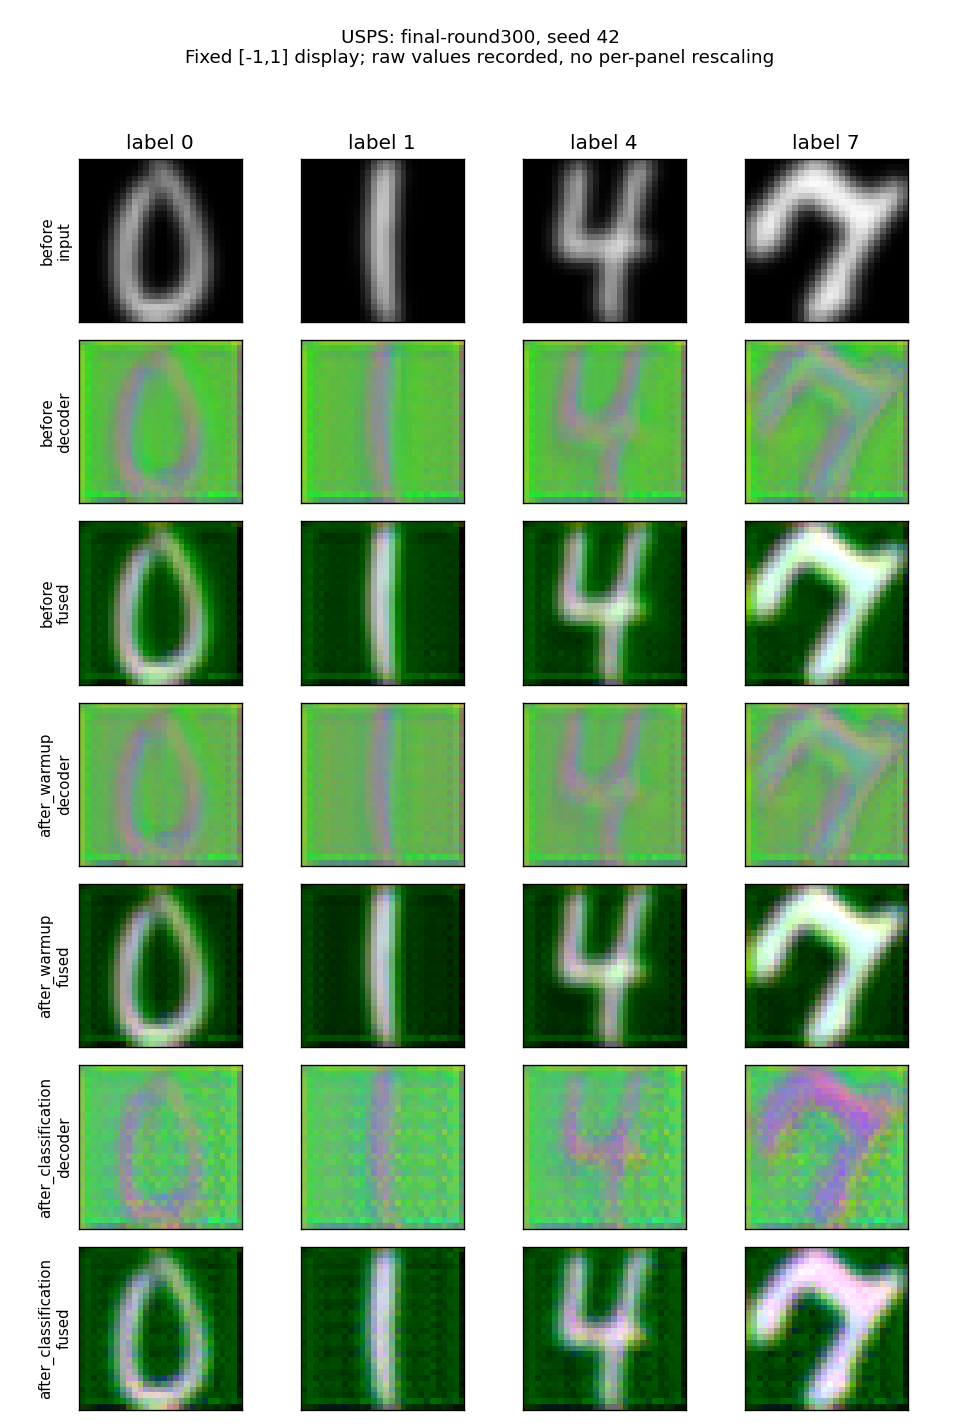
\includegraphics[width=.56in,trim=47.4bp 118.8bp 430.2bp 639.6bp,clip]{figures/digits/final-round300-USPS.png} & 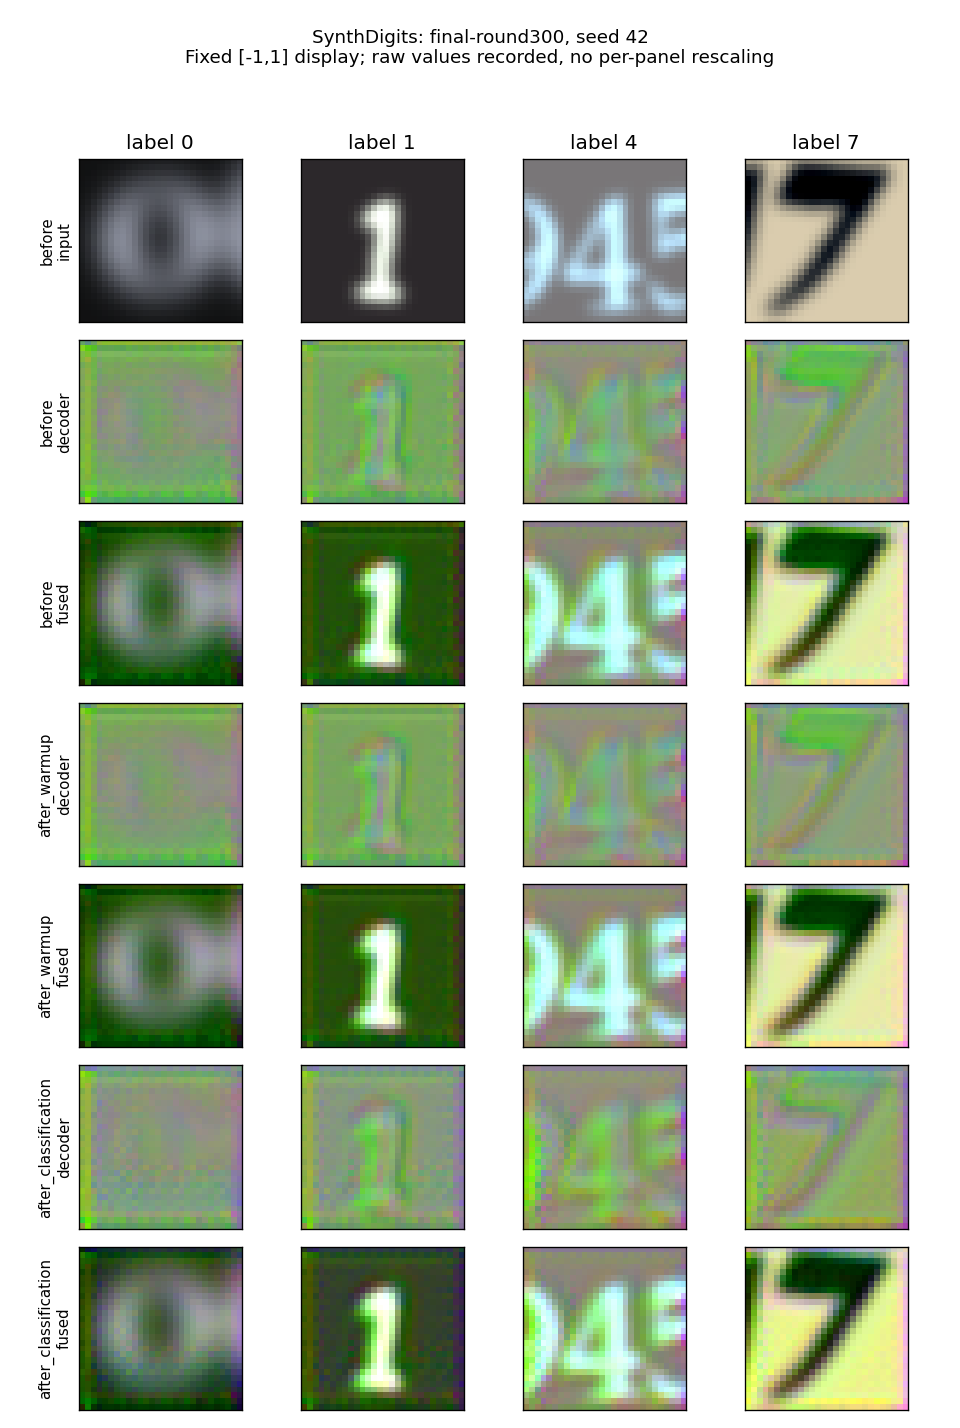
\includegraphics[width=.56in,trim=47.4bp 118.8bp 430.2bp 639.6bp,clip]{figures/digits/final-round300-SynthDigits.png} & 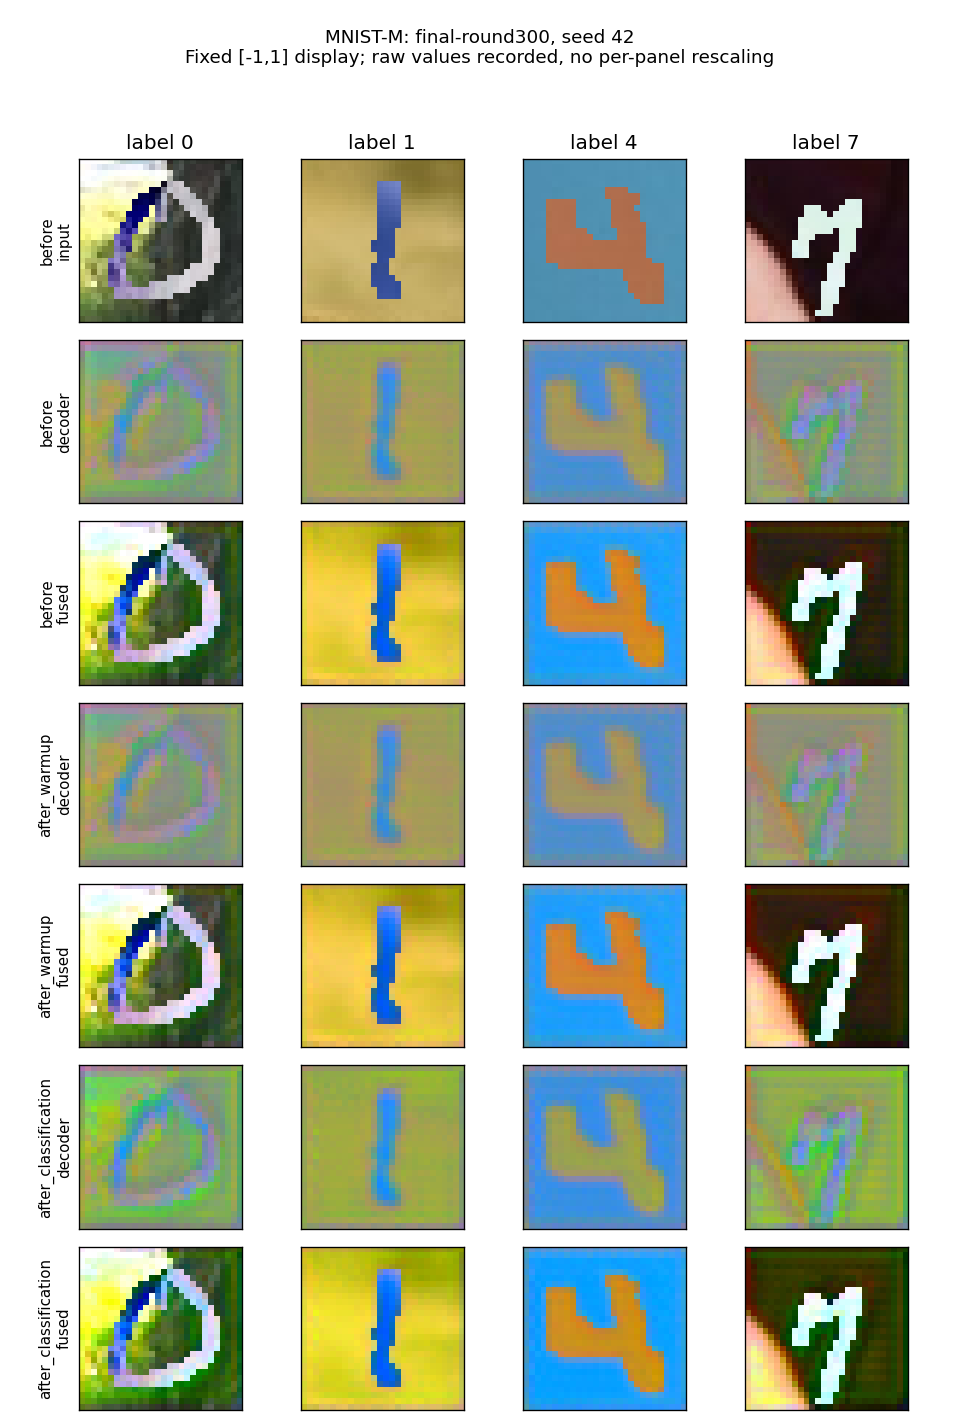
\includegraphics[width=.56in,trim=47.4bp 118.8bp 430.2bp 639.6bp,clip]{figures/digits/final-round300-MNIST-M.png} \\[-2pt]
\raisebox{.20in}{\scriptsize\shortstack[r]{After classification\\fused}} & 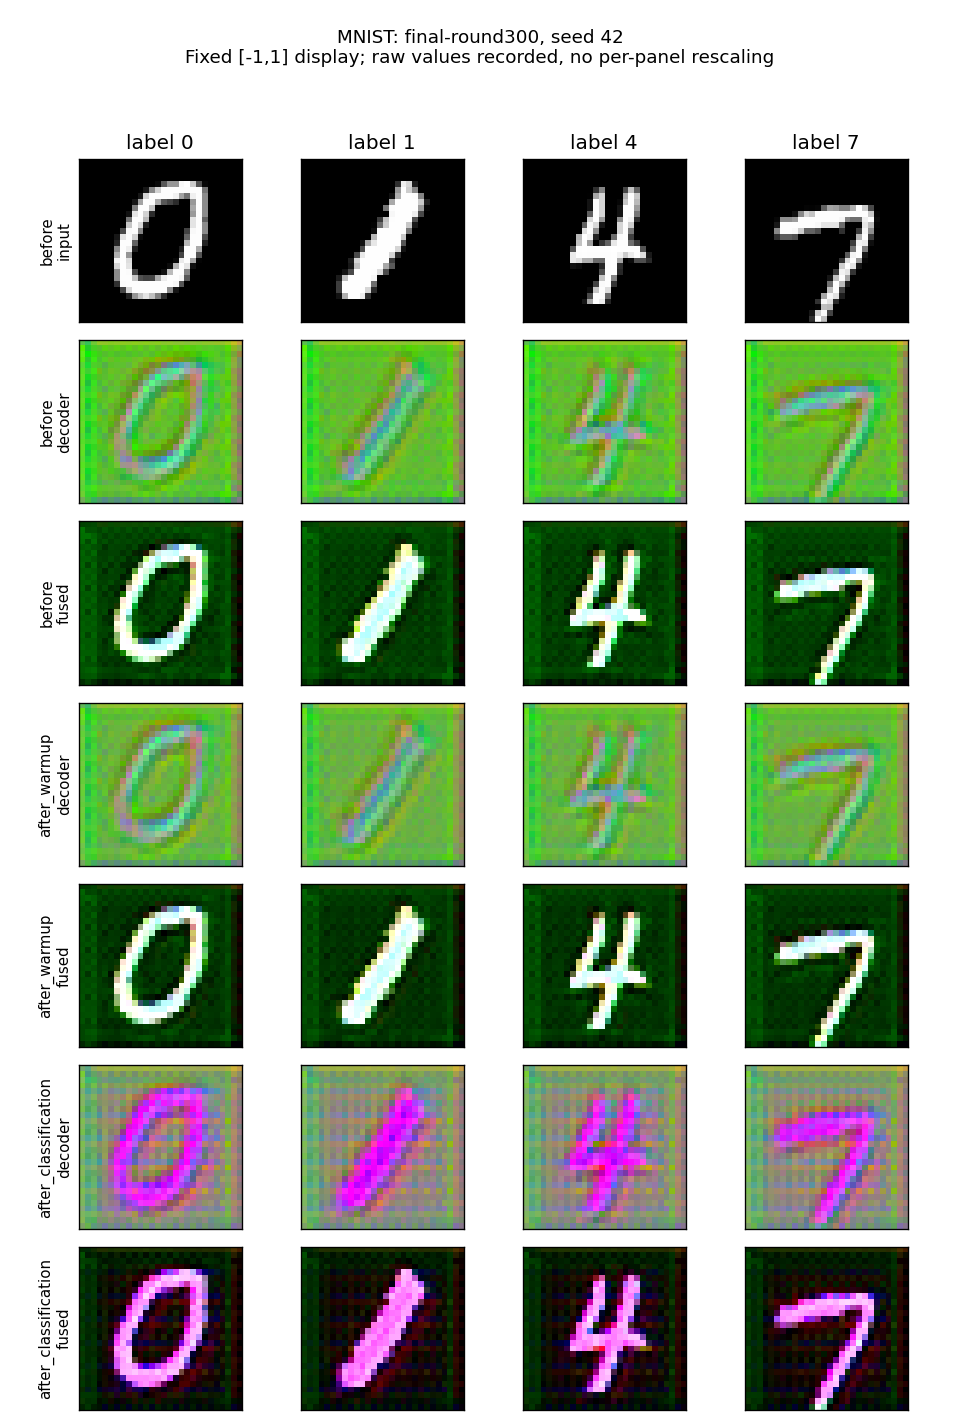
\includegraphics[width=.56in,trim=47.4bp 9.6bp 430.2bp 748.8bp,clip]{figures/digits/final-round300-MNIST.png} & 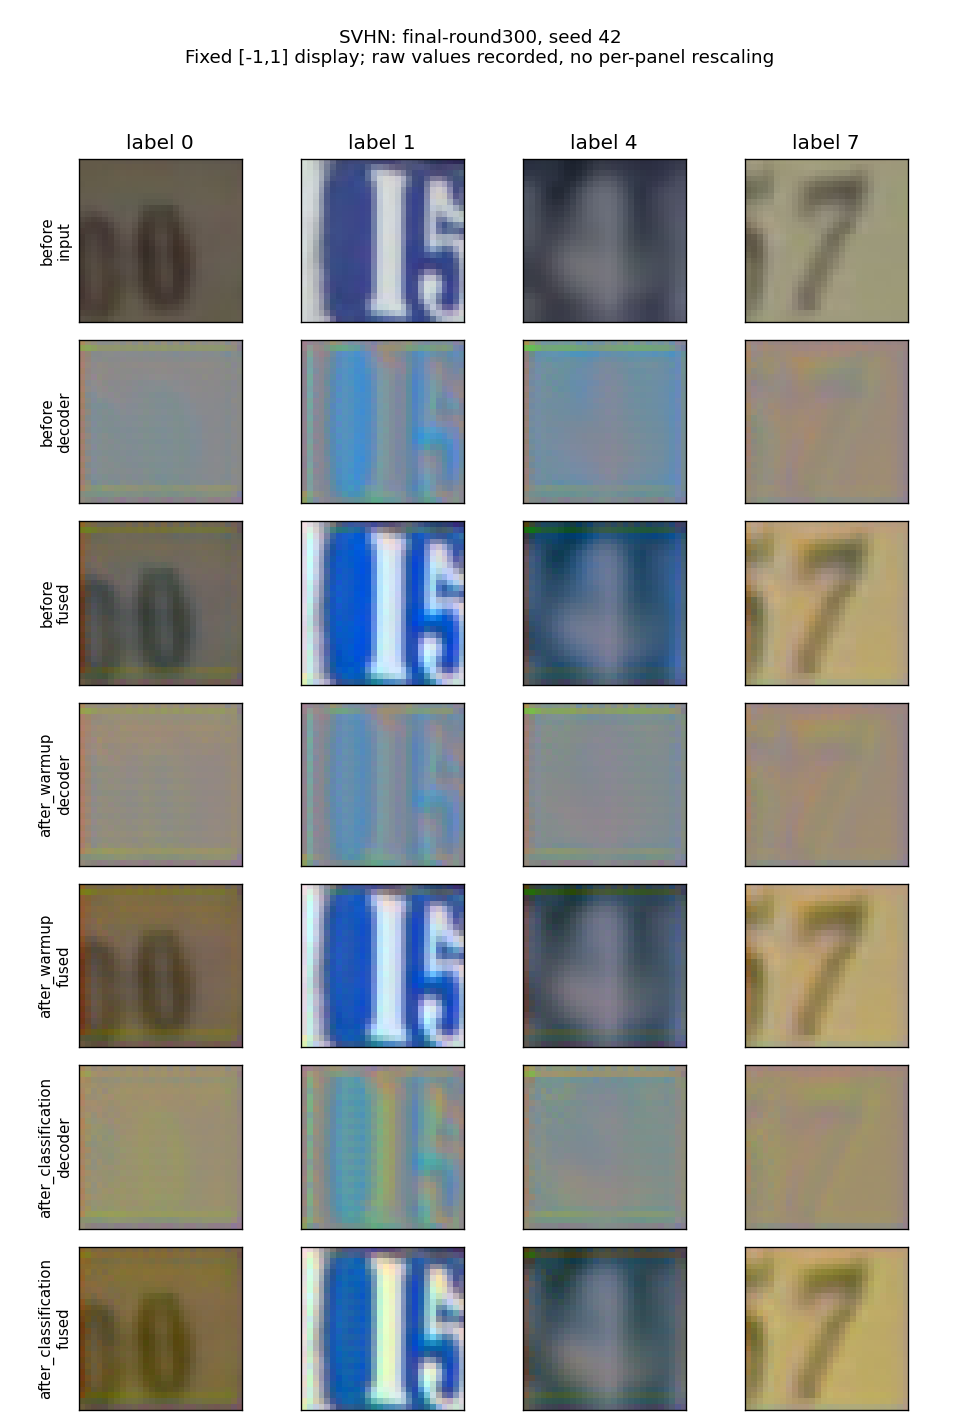
\includegraphics[width=.56in,trim=47.4bp 9.6bp 430.2bp 748.8bp,clip]{figures/digits/final-round300-SVHN.png} & 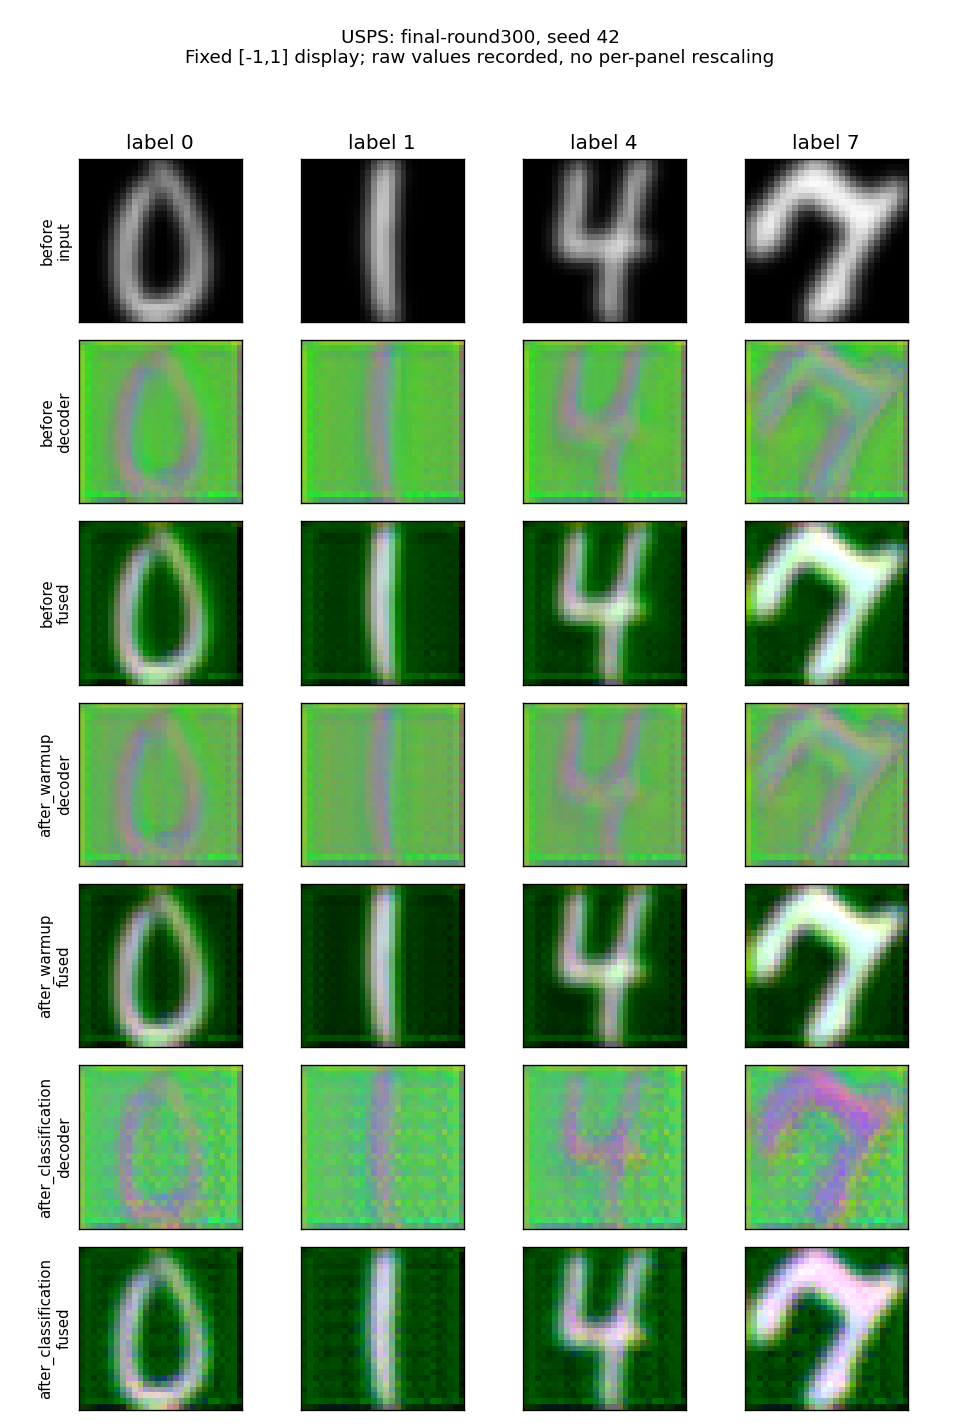
\includegraphics[width=.56in,trim=47.4bp 9.6bp 430.2bp 748.8bp,clip]{figures/digits/final-round300-USPS.png} & 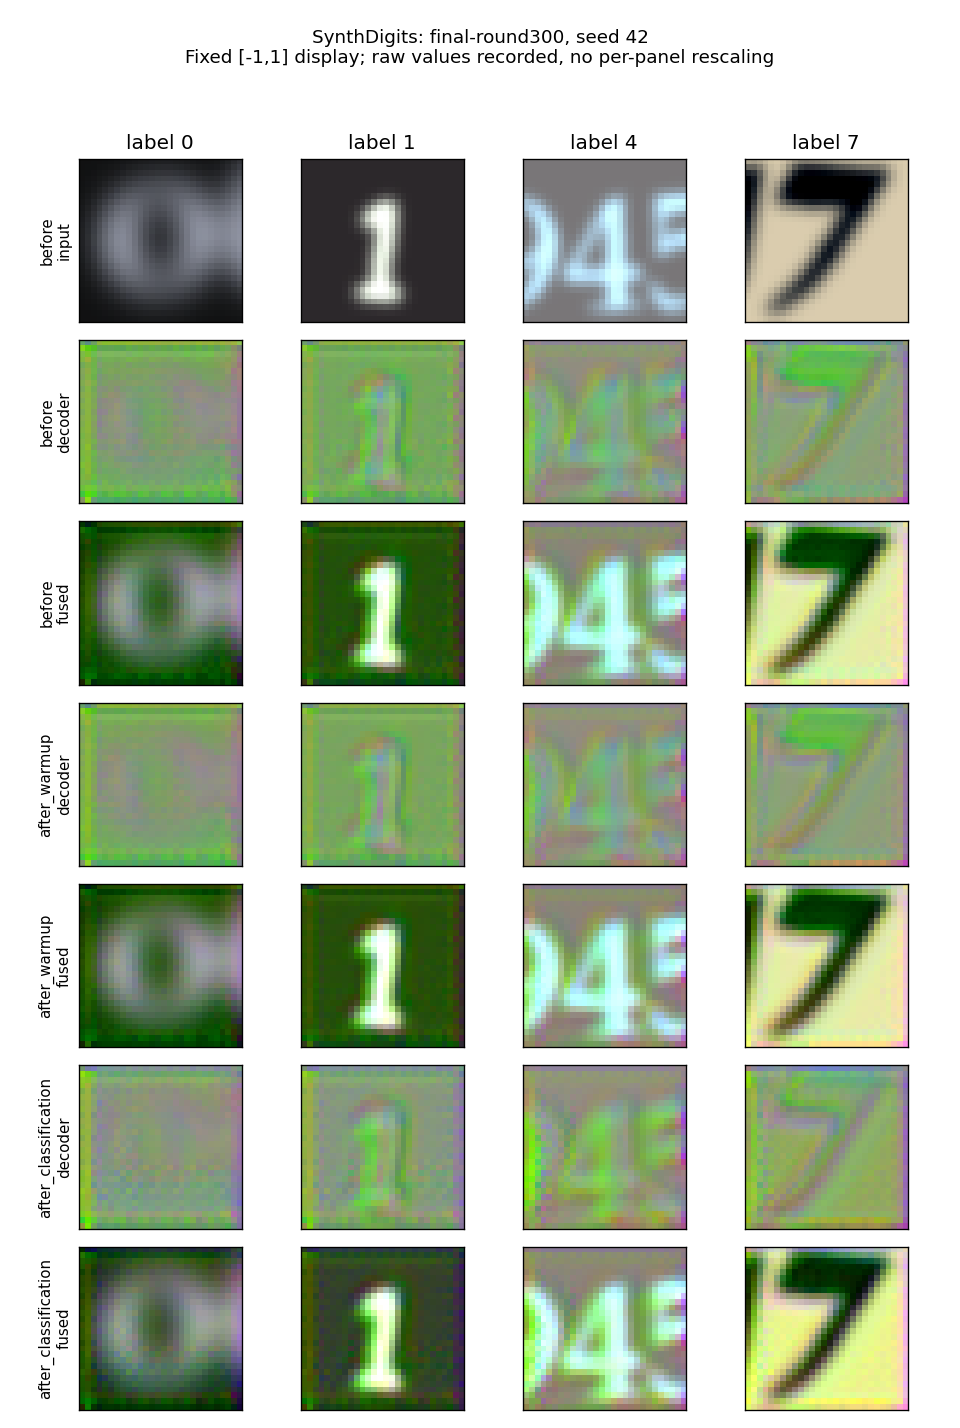
\includegraphics[width=.56in,trim=47.4bp 9.6bp 430.2bp 748.8bp,clip]{figures/digits/final-round300-SynthDigits.png} & 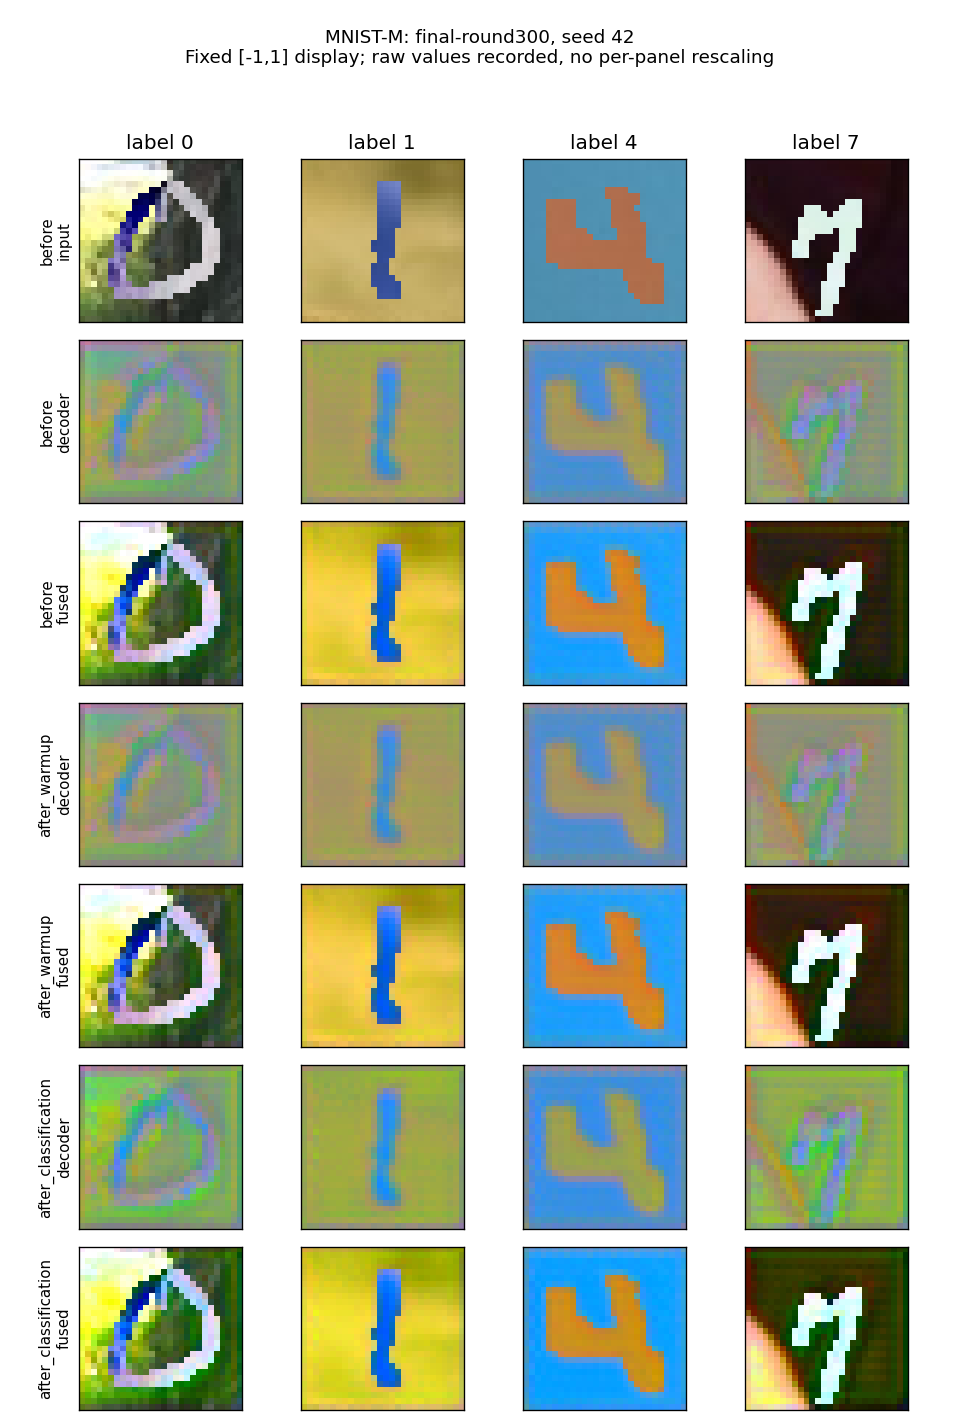
\includegraphics[width=.56in,trim=47.4bp 9.6bp 430.2bp 748.8bp,clip]{figures/digits/final-round300-MNIST-M.png} \\[-2pt]
\end{tabular}
\caption{Digits decoder probes from the final checkpoint, seed 42. Each column uses the first preselected class-0 example in that domain; the same example is shown throughout its local replay. Rows show the input and the decoder and fused outputs before adaptation, after warm-up, and after classification. All panels retain the fixed display range $[-1,1]$ of the archived grids; clipping is applied only for visualization, without panel-specific rescaling. Quantitative measurements use the raw, unclipped outputs.}
\label{fig:digits_decoder_probe}
\end{figure*}


\subsection{Component Ablations}
\label{app:digits_ablation}

How do the design choices affect the accuracy of the complete fusion
pipeline? We reuse the five full-model runs and train each of three variants
from scratch with the same five seeds, giving 15 additional runs of
300 rounds. The variants remove reconstruction warm-up, share the encoder,
or remove the original-input pathway. In the shared-encoder variant, all
clients start with the same encoder and uniformly average its state together
with the decoder and classifier after each round. The decoder-only variant
classifies $D(E_i(x))$ while retaining private encoders and warm-up.

All variants inherit the hyperparameters selected for the full pipeline,
without additional tuning: classifier SGD with learning rate 0.1,
encoder--decoder Adam with learning rate 0.0003, clipping at 10, batch size
32, and $d_z=64$. Training uses all 743 examples per domain and one
classification epoch per round; the full, shared-encoder, and decoder-only
variants additionally perform one warm-up epoch. Each final model is
evaluated once on the five domain test sets, containing 147,509 examples
in total. Uniform-domain accuracy is computed within each run.

\begin{table*}[t]
\coauthorcolor
\centering
\small
\setlength{\tabcolsep}{15pt}
\caption{Digits component ablations. Uniform-domain test accuracy at round 300 and paired differences are mean $\pm$ sample standard deviation over seeds 42--46. Positive differences favor the full pipeline. Bold marks the highest mean accuracy among the evaluated variants.}
\label{tab:digits_ablation}
\begin{tabular}{lcc}
\toprule
Variant & Uniform-domain accuracy (\%) & Full $-$ variant (pp) \\
\midrule
Full FusedSpaceFed & $85.86\pm0.85$ & -- \\
Without warm-up & $85.71\pm0.79$ & $+0.15\pm0.53$ \\
Shared encoder & $\boldsymbol{86.18\pm0.47}$ & $-0.32\pm0.58$ \\
Decoder output only & $84.86\pm0.58$ & $+1.00\pm1.22$ \\
\bottomrule
\end{tabular}
\end{table*}


Results are reported as mean $\pm$ sample standard deviation across five
paired seeds; differences are computed within each seed.
Removing warm-up also reduces the optimization budget and changes the Adam
state and minibatch order at the start of classification. This intervention
therefore measures the overall effect of removing the warm-up phase.

The complete pipeline achieves $85.86\%$ mean uniform-domain accuracy,
compared with $84.86\%$ when the original-input pathway is removed.
This 1.00-point average advantage supports combining the learned decoder
output with the original image. The no-warm-up and shared-encoder variants
obtain $85.71\%$ and $86.18\%$, respectively, showing smaller mean changes
under these interventions in the feature-heterogeneous Digits setting.

\subsection{Fixed-State Gradient Dispersion}
\label{app:digits_gradients}

Can the learned fusion pathway realize the variance--covariance reduction
condition in Equation~\eqref{eq:exact_decomp}? We compare original and fused
inputs at the initial and final checkpoints using identical classifier,
decoder, and private-encoder parameters. We use the same fixed training
probes as in Appendix~\ref{app:digits_decoder}, with no optimizer steps or
adaptation. For each client, we average the gradients of five minibatch
losses before computing cross-client dispersion.

The primary measurement freezes BatchNorm running statistics. A second
measurement uses batch statistics and restores all buffers before and after
each input pathway. These batch-statistic measurements condition the loss
on the fixed minibatches. Gradients are computed in float32 and accumulated
in float64. Table~\ref{tab:digits_gradient_decomposition} reports the terms
of the decomposition, which satisfy the identity to numerical precision.

\begin{table*}[t]
\coauthorcolor
\centering
\small
\setlength{\tabcolsep}{4pt}
\caption{Fixed-state classifier-gradient decomposition on Digits. Terms $\Gamma^{\mathrm{orig}}$, $\Gamma^{\mathrm{fused}}$, $B$, and $\Phi$ are means across five seeds. The ratio is computed within each seed and reported as mean $\pm$ sample standard deviation. The last column counts seeds satisfying $B+\Phi<0$. Frozen and Batch denote the two BatchNorm modes.}
\label{tab:digits_gradient_decomposition}
\begin{tabular}{llrrrrcc}
\toprule
Stage & BN & $\Gamma^{\mathrm{orig}}$ & $\Gamma^{\mathrm{fused}}$ & $B$ & $\Phi$ & $\Gamma^{\mathrm{fused}}/\Gamma^{\mathrm{orig}}$ & Reduced \\
\midrule
Initial & Frozen & $2.001\times10^{-2}$ & $2.012\times10^{-2}$ & $1.054\times10^{-3}$ & $-9.383\times10^{-4}$ & $1.006\pm0.013$ & 2/5 \\
Initial & Batch & $78.6571$ & $78.5144$ & $10.5506$ & $-10.6934$ & $0.998\pm0.004$ & 3/5 \\
Final & Frozen & $13.8595$ & $10.6770$ & $1.2951$ & $-4.4775$ & $0.792\pm0.253$ & 4/5 \\
Final & Batch & $6.732\times10^{-2}$ & $1.580\times10^{-3}$ & $5.700\times10^{-2}$ & $-0.1227$ & $0.148\pm0.141$ & 5/5 \\
\bottomrule
\end{tabular}

\par\vspace{10pt}
\coauthorcolor
\centering
\small
\setlength{\tabcolsep}{13pt}
\caption{Normalized and directional Digits gradient diagnostics, averaged across five seeds. Normalized dispersion is $\Gamma/(K^{-1}\sum_i\|g_i\|_2^2)$; cosine similarity is averaged over distinct pairs of client gradients. Orig.\ and Fused use identical model parameters and fixed training probes.}
\label{tab:digits_gradient_normalized}
\begin{tabular}{llrrrr}
\toprule
& & \multicolumn{2}{c}{Normalized dispersion} & \multicolumn{2}{c}{Pairwise cosine} \\
\cmidrule(lr){3-4}\cmidrule(lr){5-6}
Stage & BN & Orig. & Fused & Orig. & Fused \\
\midrule
Initial & Frozen & 0.7989 & 0.7988 & -0.0048 & -0.0049 \\
Initial & Batch & 0.7364 & 0.7370 & 0.0775 & 0.0763 \\
Final & Frozen & 0.7942 & 0.7996 & 0.0906 & 0.0440 \\
Final & Batch & 0.7966 & 0.7890 & 0.0218 & 0.0235 \\
\bottomrule
\end{tabular}
\end{table*}


At the final checkpoints, the mean per-seed ratio
$\Gamma^{\mathrm{fused}}/\Gamma^{\mathrm{orig}}$ is $0.792\pm0.253$
with frozen BatchNorm statistics and $0.148\pm0.141$ with batch statistics.
The reduction condition holds in four of five seeds and all five seeds,
respectively. These trained fusion pathways therefore provide empirical
instances of the absolute-dispersion reduction identified by the analysis.

To distinguish absolute dispersion from gradient scale and direction, we
also measure
$\Gamma/(K^{-1}\sum_i\|g_i\|_2^2)$ and the mean pairwise cosine similarity
of client gradients (Table~\ref{tab:digits_gradient_normalized}).
With frozen statistics, final-state normalized dispersion changes from
0.7942 to 0.7996 and mean pairwise cosine similarity from 0.0906 to 0.0440.
With batch statistics, the corresponding values change from 0.7966 to
0.7890 and from 0.0218 to 0.0235.
These results characterize a reduction in absolute dispersion, with
substantial sensitivity to gradient scale and BatchNorm statistics.
Both input pathways are evaluated at the same FusedSpaceFed state, whose
classifier was trained on fused inputs. Thus, the original-input pathway
is a fixed-state counterfactual; the cross-method measurements in
Section~\ref{sec:experiments} instead use each method's own final state.

\begin{coauthorchange}
\let\coauthorcolor\coauthordiffcolor
% Source: research/pathmnist_federated_head/FEDERATED_HEAD_REPORT.md,
% results commit eff87948e9fc95fd4163b0746cb7e18c910cdb86.
\clearpage
\section{Federated Classifier Refinement on PathMNIST}
\label{app:pathmnist_head_refinement}

Classifier calibration after federated training has previously been studied
under data heterogeneity~\citep{luo2021nofear}. We explore this direction for
FusedSpaceFed by refining its final linear classification layer while keeping
the learned representation fixed.

We start from the original round-50 PathMNIST checkpoint for seed 42,
trained with mixed precision using ten clients and two classes per client.
Private encoders, the shared decoder, the classifier backbone, and all
BatchNorm buffers remain unchanged. Only the 585 parameters of the final
64-to-9 linear layer are optimized, starting from their checkpoint values.

In a federated simulation with separate client processes, each client computes
frozen features from its own training images using its private encoder.
The server broadcasts candidate head parameters and receives only local losses
and head gradients. Uniform averaging across clients implements the mean
client cross-entropy objective without pooling features or labels.
Optimization uses FP32 L-BFGS with learning rate 1, strong-Wolfe line search,
history size 20, and a fixed budget of 100 iterations. The refined head is
frozen before test evaluation.

% Keep the results together in the second column of this final appendix page.
\newpage
\begin{table}[ht]
\coauthorcolor
\centering
\caption{PathMNIST head refinement from the same original checkpoint
(seed 42, round 50). Accuracy is averaged uniformly over ten
client-conditioned predictors, each evaluated on the same 7,180 official
test images. All entries concern a single seed.}
\label{tab:pathmnist_head_refinement}
\begin{tabular}{@{}p{0.67\columnwidth}r@{}}
\toprule
Model & Accuracy (\%) \\
\midrule
Original FusedSpaceFed checkpoint & 39.62 \\
Centralized head refinement, pooled training features & 75.33 \\
Federated head refinement, client-local training features & \textbf{75.46} \\
\bottomrule
\end{tabular}
\end{table}

Federated refinement improves accuracy by 35.84 percentage points
(Table~\ref{tab:pathmnist_head_refinement}). It requires 107 additional
full-participation gradient aggregations, corresponding to 5.01 MB of
bidirectional optimization payload, excluding initial model distribution
and transport overhead.

Loss and gradient checks at common parameter values satisfy the prespecified
tolerances against the centralized reference. The two truncated optimization
runs nevertheless produce different terminal models, with 2.36\% disagreement
in test predictions, and do not satisfy the stricter terminal-equivalence
criteria.

This experiment shows that substantial predictive performance can be recovered
through final-layer optimization while preserving client-local data processing.
The single-seed result motivates further evaluation of this additional
federated stage across seeds, datasets, and communication budgets.

\end{coauthorchange}
\end{coauthorrevision}

\end{document}
